\newif \ifDraft         \Draftfalse

\Drafttrue

% \newcommand{\Release}{Release 0.2, 2022-10-03}
% Release 0.2: changeset 553cd65913097b9a73a43ea291ab29fc2768887d

% Release 0.3 skipped (internal)

%\newcommand{\Release}{Release 0.4, 2024-03-27}
% Release 0.4: changeset c65bf1042 aka RELEASE_0_4

%\newcommand{\Release}{Release 0.5, 2024-08-06}
% Release 0.5: changeset f2d767f aka RELEASE_0_5

%\newcommand{\Release}{Release 0.6, 2025-03-21}
% Release 0.6: changeset 909d280b aka RELEASE_0_6

\newcommand{\Release}{Draft Release 0.7}


\documentclass[a4paper,12pt]{report}
\usepackage[copyright]{unsw}
\copyYear{2022, 2024}
\Unit{School of Computer Science \& Engineering}
\SubUnit{Trustworthy Systems Group}

\usepackage[square,sort&compress,authoryear]{natbib}
%\usepackage[pdftex]{hyperref}
\usepackage{tabularx}
\usepackage{xspace}
\usepackage{verbatim}
\usepackage{datetime}
\usepackage{listings}

% Acronyms
\usepackage[acronym]{glossaries-extra}
%\setabbreviationstyle[acronym]
%\setacronymstyle{long-short}
\makenoidxglossaries

% Get bibliography into the ToC
\usepackage[nottoc]{tocbibind}
% Get listings into the ToC
\renewcommand{\lstlistoflistings}{\begingroup
    \tocfile{List of Listings}{lol}
\endgroup}

\usepackage{tikz}
\newcommand*\circled[1]{\tikz[baseline=(char.base)]{
            \node[shape=circle,draw,inner sep=0pt,thick] (char) {#1};}}


% use a reasonably looking fixed-width font
\usepackage[T1]{fontenc}
\usepackage[scaled=0.82]{beramono}

% Leave this in here, it is often useful to deal with latexdiff breakage.
% Put it around breakage-causing segments (in both versions to be diffed!)
\newenvironment{DIFnomarkup}{}{}

\setkeys{Gin}{keepaspectratio=true,clip=true,draft=false}
\graphicspath{{./imgs/}}

\lstset{
  language=C,
  basicstyle=\ttfamily,
  numbers=left,
  numberstyle=\tiny,
  xleftmargin=17pt,
  captionpos=b,
  escapeinside={(@}{@)},
  showstringspaces=false
}

\ifDraft
  \usepackage{draftwatermark}
  \SetWatermarkLightness{0.85}
  \newcommand{\Comment}[1]{\textbf{\textsl{#1}}}
  \newenvironment{LongComment}[1] % multi-paragraph comment, argument is owner
    {\begingroup\par\noindent\slshape \textbf{\colorbox{yellow}{Begin Comment[#1]}}\par}
    {\par\noindent\textbf{\colorbox{yellow}{End Comment}}\endgroup\par}
  \newcommand{\FIXME}[1]{\textbf{\textsl{\colorbox{yellow}{FIXME:} #1}}}
  \newcommand{\TODO}[1]{\textbf{\textsl{\colorbox{yellow}{TODO:} #1}}}
  \newcommand{\DEFER}[1]{\textbf{\textsl{\colorbox{magenta}{DEFER:} #1}}}
  \newcommand{\IOU}[1]{\textbf{\textsl{\colorbox{yellow}{IOU:} #1}}}
  \newenvironment{Confirm}{\begingroup\color{red}\textbf{\textlangle\!\textlangle\!\textlangle\!\textlangle}}{\textbf{\textrangle\!\textrangle\!\textrangle\!\textrangle}\endgroup}
\else
  \newcommand{\Comment}[1]{\relax}
  \newenvironment{LongComment}[1]{\expandafter\comment}{\expandafter\endcomment}
  \newcommand{\FIXME}[1]{\relax}
  \newcommand{\TODO}[1]{\relax}
  \newcommand{\DEFER}[1]{\relax}
  \newcommand{\IOU}[1]{\relax}
  \newenvironment{Confirm}{\relax}{\relax}
\fi

% This sort of command for each active author can be convenient
\newcommand{\gernot}[1]{\Comment{#1 \colorbox{yellow}{[gernot]}}}
\newcommand{\kevin}[1]{\Comment{#1 \colorbox{yellow}{[kevin]}}}
\newcommand{\lucy}[1]{\Comment{#1 \colorbox{yellow}{[lucy]}}}
\newcommand{\courtney}[1]{\Comment{#1 \colorbox{pink}{[Courtney]}}}
\newcommand{\peterc}[1]{\Comment{#1 \colorbox{yellow}{[peterc]}}}
\newcommand{\IoU}[1]{\Comment{\colorbox{yellow}{Obligation:} #1}}

\newcommand{\ToCome}[1]{\textbf{#1 to come.}}

\newcommand{\code}[1]{\texttt{#1}}
\newcommand{\Obj}[1]{\textsl{#1}}

\newcommand{\Ra}{R\(_{\mbox{\footnotesize a}}\)\xspace}
\newcommand{\Tc}{T\(_{\mbox{\footnotesize c}}\)\xspace}
\newcommand{\Ta}{T\(_{\mbox{\footnotesize a}}\)\xspace}
%\newcommand{\Ba}{B\(_{\mbox{\footnotesize a}}\)\xspace}
%\newcommand{\Bf}{B\(_{\mbox{\footnotesize f}}\)\xspace}
\newcommand{\Rq}{R\(_{\mbox{\footnotesize q}}\)\xspace}
\newcommand{\Rf}{R\(_{\mbox{\footnotesize f}}\)\xspace}

\newacronym[shortplural={OSes}]{os}{OS}{operating system}
\newacronym{sddf}{sDDF}{seL4 Device Driver Framework}
\newacronym{api}{API}{application programming interface}
\newacronym{tcb}{TCB}{trusted computing base}
\newacronym{cpu}{CPU}{central processing unit}
\newacronym{mmu}{MMU}{memory management unit}
\newacronym{io}{I/O}{input/output}
\newacronym{iommu}{IOMMU}{input/output memory management unit}
\newacronym{dma}{DMA}{direct memory access}
\newacronym{mmio}{MMIO}{memory-mapped I/O}
\newacronym{uio}{UIO}{Linux userspace I/O}
\newacronym{virtio}{VirtIO}{Linux I/O virtualisation framework}
\newacronym{irq}{IRQ}{interrupt request}
\newacronym{vspace}{VSpace}{virtual address space}
\newacronym{cspace}{CSpace}{capability address space}
\newacronym{nic}{NIC}{network interface card}
\newacronym{tx}{Tx}{transmit}
\newacronym{rx}{Rx}{receive}
\newacronym{rq}{Rq}{request}
\newacronym{rs}{Rs}{response}
\newacronym{sc}{SC}{scheduling context}
\newacronym{cdrom}{CD-ROM}{compact-disk read-only memory}
\newacronym{vm}{VM}{virtual machine}
\newacronym{vmm}{VM}{virtual-machine monitor}
\newacronym{pcm}{PCM}{pulse-code modulation}
\newacronym{phy}{PCM}{physical layer}
\newacronym{camkes}{CAmkES}{component architecture for
  microkernel-based embedded systems, a user-level framework for
  developing on top of seL4}
\newacronym{i2c}{I2C}{Inter-Integrated Circuit (serial communication bus)}
\newacronym{ppc}{PPC}{seL4 protected procedure call}
\newacronym{pd}{PD}{Protection Domain: a virtual address space plus a
  thread of control.  A PD roughly corresponds to a Unix process.}
\newcounter{Qi}\setcounter{Qi}{0}
\newcounter{Qii}
\newenvironment{Question}[1][]    % research question, arg is intro before list
%{\begingroup\setcounter{QuestII}{1}\addtocounter{QuestI}{1}%
{\addtocounter{Qi}{1}\par%
  \textbf{Research Question~\arabic{Qi}.:} \emph{#1} Considerations:
  \begin{list}{\textbf{C\arabic{Qi}.\arabic{Qii}:}}%
    {\setlength\labelsep{8pt}%
      \setlength\itemindent{0pt}%
      \setlength\leftmargin{40pt}%
      \setlength\labelwidth{33pt}%
      \usecounter{Qii}}}%
{\end{list}}

% Scale figs to match font sizes
\newcommand{\figscale}{0.2}

\begin{document}
%% Capitalisation of cross references
\newcommand{\lstnumberautorefname}{Line}
\renewcommand{\chapterautorefname}{Chapter}
\renewcommand{\sectionautorefname}{Section}
\renewcommand{\subsectionautorefname}{Section}
\renewcommand{\subsubsectionautorefname}{Section}
\renewcommand{\appendixautorefname}{Appendix}
\renewcommand{\Hfootnoteautorefname}{Footnote}

\setcounter{topnumber}{2}
\renewcommand{\topfraction}{0.91}

\pagenumbering{roman}

\title{sDDF Design}
\SubTitle{Design, Implementation and Evaluation of the\\ seL4 Device Driver Framework}
\author{Gernot Heiser, Peter Chubb, Alex Brown, Julia Broady, Courtney Darville, Lucy Parker}
\Email{gernot@unsw.edu.au}
\date{\Release \ifDraft\ of \today\fi}
\maketitle

\subsection*{Abstract}

This is a work-in-progress report that documents the design of a
high-performance device driver framework for seL4, including the
structure and interfaces of compliant drivers, and presents some
preliminary evaluation.

The document is intentionally explicit about the assumptions it makes on
hardware (the \emph{device model}) and the structure it prescribes on
device drivers (the \emph{driver model}). This is to
facilitate exploring formal specification and, eventually,
verification of device drivers.

Consequently, besides specifying how drivers and their interfaces are
structured, the document also serves to define the context for the
\emph{Pancake} project that develops a programming language for
verifiable device drivers. As such, the report serves as an informal
interface document between the Pancake team and systems researchers
(and thus explains many things systems people take for granted).

\tableofcontents
\listoffigures
%\listoftables
\lstlistoflistings
\printnoidxglossaries

\chapter{Aims of the sDDF}\label{s:aims}
\pagenumbering{arabic}

Every operating system (\gls{os}) needs device drivers, and \glspl{os} based on the seL4
microkernel~\citep{Klein_EHACDEEKNSTW_09, sel4:URL} are no exception.

The seL4 Device Driver Framework (\gls{sddf}) provides libraries, interface specifications and tools
for writing/porting device drivers to run as native, isolated
components on seL4. Specifically, the \gls{sddf} design aims to:
\begin{itemize}
\item support a wide class of devices, including network, USB,
  graphics, storage, serial ports etc;
\item achieve performance comparable
  to Linux in-kernel drivers, as measured by throughput, latency and \gls{cpu}
  load, at least for latency-sensitive  high-throughput devices
  (network interface cards and USB);
\item  be robust against  defined threats;
\item support sharing of devices between multiple clients, which might be
  seL4-native components or virtual machines;
\item provide strong \emph{separation of concerns};
\item eventually enable the formal verification of its components.
\end{itemize}

The \gls{sddf} assumes a general  \hyperref[s:device]{device model} that should enable
formal reasoning. It defines a \hyperref[s:driver]{device driver model}
that is appropriate for seL4 and aims to simplify driver
implementation, eliminate common causes of driver bugs and aid formal
verification. It is based on an asynchronous, zero-copy \hyperref[s:transport]{transport
  layer} that minimises overheads while keeping driver interfaces simple.

For the time being we focus on defining a driver model and its control
and data interfaces to the driver's clients, leaving other required
functionality, such as device discovery and device initialisation for
future work.


\chapter{Threat Model}\label{s:threats}

The ultimate aim is a system whose whole \emph{trusted computing base}
(\gls{tcb}) is verified to be \emph{trustworthy}. This requires the \gls{tcb} to be
minimised. An implication is that some drivers will be part of the \gls{tcb}
and thus trusted, while others (the majority) of drivers are not. It
also means that the driver framework itself is trusted.

We assume that an attacker is able to compromise and fully control any
component that is not part of the \gls{tcb}. Specifically this means that
\textbf{the attacker may:}
\begin{itemize}
\item execute arbitrary instructions in the address
  space of any untrusted driver;
\item execute arbitrary instructions in the address
  space of any untrusted client;
\item arbitrarily change the data on untrusted external media
  (network or physically insecure storage).
\end{itemize}

However, \textbf{the attacker cannot:}
\begin{itemize}
\item compromise a trusted component (driver, virtualiser);
\item compromise a trusted client;
\item compromise the driver framework itself.
\end{itemize}

We assume that trusted clients or servers dealing with untrusted
entities use encryption protocols, such as TLS, to ensure
confidentiality and integrity of data, even if using untrusted
components. If a client only employs trusted components,
the system must guarantee confidentiality, integrity and availability.

The threat model implies that it must be feasible to formally verify
all trusted components (eventually).

\chapter{Device Model}\label{s:device}

\begin{figure}[th]
  \centering
  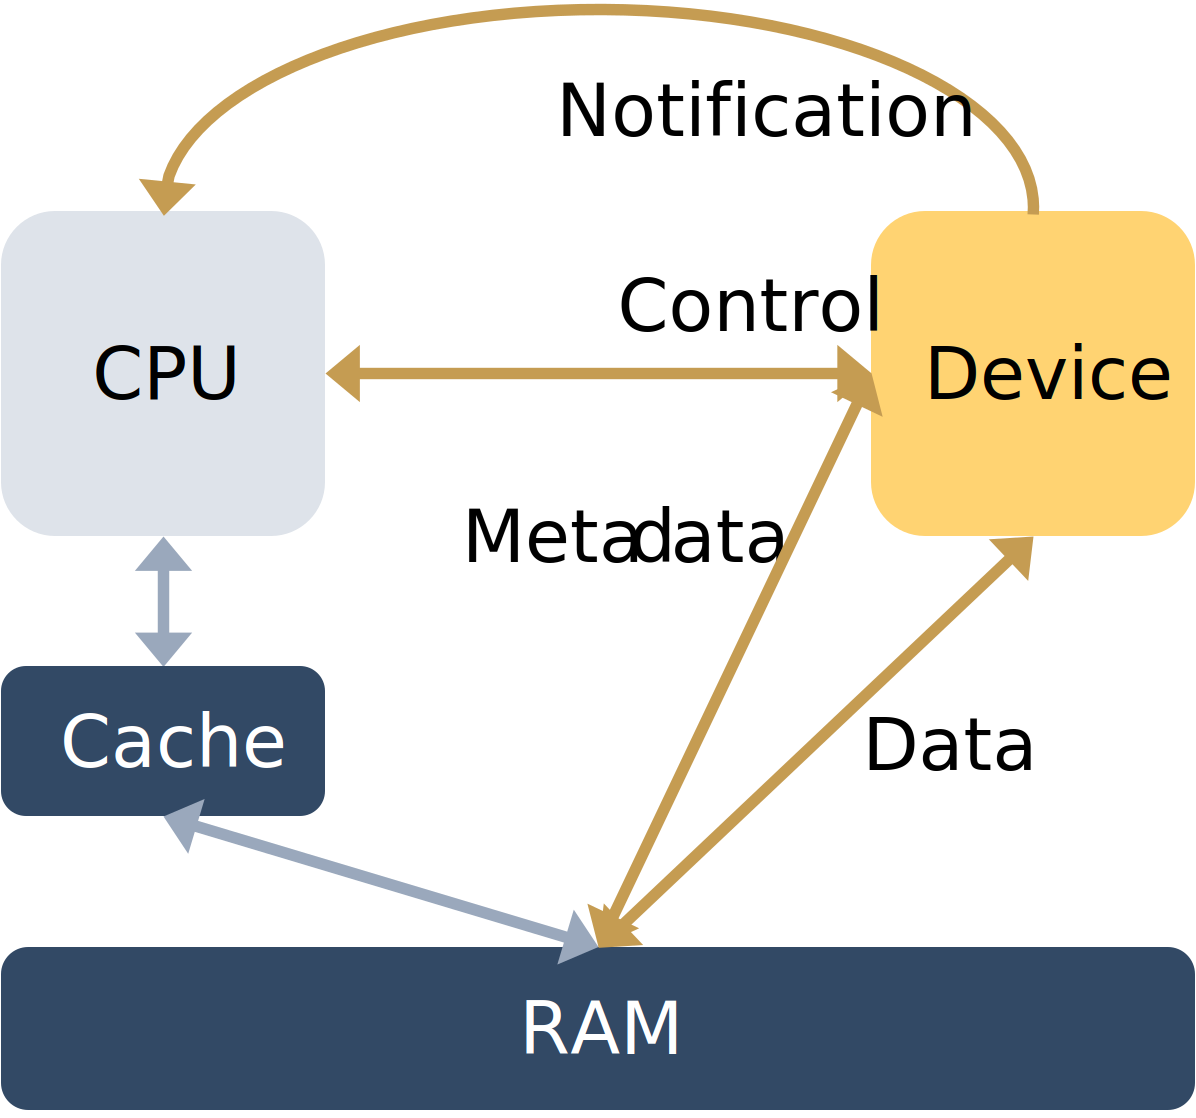
\includegraphics[scale=\figscale]{device}
  \caption{Device model.}
  \label{f:device}
\end{figure}

We view a device as a state machine (implemented in hardware) with four interfaces, indicated
in \autoref{f:device}:
\begin{description}
\item[the control interface] specifies how the software running on the
  \gls{cpu}, i.e.\ the \emph{device driver}, issues commands to
  the device, and how the device reports status information back to the driver;
\item [the notification interface] lets the device alert the driver to a
  state change;
\item [the data interface] transports data between software and the
  device;
\item[the metadata interface] specifies data locations and is
  referenced by the control interface.
\end{description}

The notification interface is one-way (device to driver) while the
control interface is two-way. The data interface can be one-way: for a
pure  input device (microphones, cameras, read-only storage media), data only travels from
the device to the driver, while for a pure output device
(audio output, display), data only
travels from the driver to the device; other devices (network,
storage) have two-way data interfaces. The metadata interface is
two-way, as for both input and output channels it is updated by both
sides.

The model is presently somewhat simplified, in that it does not take
into account hot-plugging/unplugging (important e.g.\ for USB devices),
nor the possibility of separate \gls{dma} controllers.

\DEFER{\gls{dma} to/from RAM may be done by a separate \gls{dma} controller,
  which has its own driver. Shared \gls{dma} controller not on any devices
  we're presently dealing with, ignoring for now.}

\section{Device interfaces}

The \textbf{control interface} is memory-mapped: The driver accesses the
interface by reading from or writing to specific physical addresses,
\emph{device registers}, which are mapped (by the memory management
unit, \gls{mmu}) into the driver's virtual address space.%
\footnote{On the x86 architecture some legacy devices, specifically
  serial ports, are not memory mapped and require \gls{io} port instructions to
  control.  These devices process small amounts of data (have no data
  interface) and are not performance-critical. They will be handled in
  an ad-hoc manner.}

\emph{These device
registers do \emph{not} behave like regular memory!} Specifically:
\begin{itemize}
\item a write to a device register followed by a read from the same
  register might \emph{not} return the value written (and may result
  in an error condition);
\item the sequence of reads or writes matters: the outcome may change
  if register accesses are reordered;
\item the granularity of device register accesses matters: a byte-sized write to a register address
  followed by three byte-sized writes to subsequent addresses might not
  have the same effect as a 32-bit write to the same address.
\item multiple reads or writes to the \emph{same} address are all
  significant, and can have a user-visible effect, even if the values
  read/written are identical.
\end{itemize}
Among others, these properties require that device registers are
mapped uncached, and that software declares them \code{volatile}. The
correct granularity and sequence of device register accesses are
defined by the \hyperref[s:dev_proto]{device interface protocol}.

The \textbf{notification interface} is an interrupt (which the seL4 kernel
converts into signalling a \Obj{notification} object). It instructs
the driver to use the control interface to determine
what is being notified. Interrupts can signal a number of conditions:
\begin{itemize}
\item \textbf{transmit completed:} the device has completed an output (data
  write) operation and will no longer access the relevant output data;
\item \textbf{data available:} the device has completed an input (data read)
  operation, will no longer access the respective buffer and software
  can now safely access the data;
\item \textbf{other state changes:} the device state has changed in
  some other way, which includes such events as disk spin up
  completed, network cable inserted, firmware download completed;
\item \textbf{error:} some failure occurred (which includes a device losing
  power or being disconnected).
\end{itemize}

The \textbf{data} and \textbf{metadata interfaces} use
actual memory (called \emph{direct memory access},
\gls{dma}). This means that the device accesses the memory concurrently with software, similar to a separate
processor core. This has a number of implications:
\begin{itemize}
\item \gls{dma} generally bypasses the cache. While some processors (specifically the
  x86 architecture) hides this fact by ensuring the cache remains
  coherent with \gls{dma} memory, others (specifically Arm) do not,
  requiring the use of memory barriers for consistency, and the use of
  cache-management operations (cache flush or invalidate).
\item Software must not read \gls{dma} memory while an input is in progress,
  and must not write \gls{dma} memory while an output is in progress.  In
  fact, because reads and writes affect the cache, it is advisable not
  to perform any reads or writes to a \gls{dma} buffer during \gls{io} to that
  buffer.
\item Speculative reads (aka.\ pre-fetching) on \gls{dma} memory may happen
  while the device is writing input data, requiring extra cache
  management on input buffers.
\item Addresses used for \gls{dma} are either not mapped (i.e., they are
  physical addresses), or are mapped via a different \gls{mmu}, the \gls{iommu},
  from the addresses used by the \gls{cpu}.
\item For the \Obj{metadata region}, explicit cache management is
  usually not worthwhile, meaning that the \gls{cpu} should map this memory
  \emph{uncached} (unless the hardware maintains cache coherency, as
  on x86).
\end{itemize}

Simple devices (serial port, timers) do not usually use \gls{dma}. We can treat them
as the special case of an empty data and metadata interface.

\section{Device interface protocol}\label{s:dev_proto}

Software access to device registers (writes and potentially reads)
trigger state transitions in the device; a device state transition may
result in a software-visible change in a device register.

The device interface protocol specifies the addresses, sizes and
semantics (i.e.\ state transitions triggered by access) of device
registers. It also specifies some ordering conditions on accesses
(reads or writes). It
may specify timing conditions on accesses.

Examples of timing conditions are:
\begin{itemize}
\item  access \(B\) must happen no earlier than \(x\) microseconds after
  access \(A\);
\item after access \(A\), the driver must poll (read) register \(b\) until it
  is non-zero, before performing access \(C\).
\end{itemize}

For the case that the protocol specifies minimal delays between
accesses, we can assume that there are only a small number of such
delay values, which are calibrated at device setup time and are
abstracted by delay functions defined outside the driver proper.

\section{Device operation}

A sequence of state transitions may move the device into a state
where it performs \textbf{output}, by reading \gls{dma} memory. Specifically it will
follow references, supplied by the control interface, to descriptors
in \gls{dma} memory (the metadata interface), and from there to the actual
data (data interface). Addresses for \gls{dma} have to be translated to the
device address space before being given to the device. The device may
use physical addresses or its own virtual address space (mapped by the \gls{iommu}).

The completion of the output operation
results in a state transition that triggers the notification interface
(i.e.\ an interrupt); the driver then needs to use the control
interface to determine the reason for the interrupt (i.e.\ output
completed).

A sequence of state transitions may move the device to a state where
it can provide \textbf{input} to \gls{dma} buffers provided by the driver via the metadata
interface, which in turn was referenced by the control interface. To
software, the commencement of input is
non-deterministic (it is determined by the environment). The completion of
input results in a state transition that triggers the notification
interface, the driver then needs to use the control interface to
determine the reason for the interrupt (i.e.\ data available).

Once an interrupt has triggered, the hardware disables the interrupt
(and lower-priority ones), preventing it from re-occurring if it is a
level-triggered interrupt. The kernel
immediately masks that specific interrupt (preventing
it from triggering again) and then acknowledges it (which re-enables
all the lower priority ones).
When the driver \emph{acknowledges} the interrupt to the
kernel, the kernel unmasks the interrupt, after which the driver can
wait for the next interrupt.

A single interrupt
may signal multiple completions (this is called \emph{interrupt
  coalescing}). The driver needs to process all pending completions
prior to acknowledging the interrupt. Depending on the device, the
driver may also have to clear interrupt conditions in the device
registers to prevent the interrupt re-triggering.

Completions can continue to occur while interrupts are masked, which
implies that upon acknowledging, the interrupt may immediately trigger
again, resulting in the driver immediately receiving a new
notification as soon as it finished processing the present one. In
order to minimise the number of kernel entries, the driver should,
before acknowledging the \gls{irq}, use the device's control interface to
check for pending interrupts. After processing all pending events,
the driver clears the device's event register. (Note: this is a performance
optimisation, not a correctness issue.)

If interrupts are masked for too long, or software is too slow to
process input data, the device will run out of free \gls{dma} buffers
for depositing input data; in this case data will be lost
(the device drops packets). This creates an automatic flow control of inputs,
and can be used to prevent overloading the system (called \emph{rate
  limiting} the device).

Network packets can be lost for external reasons too, e.g.\ in a
router between source and destination, or by interference on a
wireless link. Higher-level network protocols
(e.g.\ TCP) handle packet loss using acknowledgement and re-transmission.

We ignore error conditions for now, but note that dropping of packets
is not considered an error condition.

Devices that can be plugged into or removed from a running system,
such as USB devices or SD cards, add further complications which we
ignore for now. Support for ``hotplugging'' will be covered in
\autoref{s:hotplugging}.

\DEFER{Error conditions should be signalled to the Monitor to deal
  with. Leave for now.\\
  Also, the device info page we presently have for storage should be
  extended to NW, e.g. for monitoring dropped-packet rates. Leave for now.}

\section{Comments}

The device interface protocol is defined by the hardware, and is thus not
under our control. To enable formal reasoning about driver
correctness, the device protocol will have to be formalised.

Unfortunately, these protocols are usually specified in manufacturers'
data sheets that are highly informal, typically vague, and frequently
wrong. Errors in data sheets arise from device implementation bugs as
well a manufacturer-internal miscommunication between hardware
designers and documenters. Even worse, there are many cases where not
even a data sheet is available, and the interface is
reverse-engineered from a Linux driver implementation.

Buggy device interface specs will inherently lead to buggy
drivers. Unfortunately, this is not something we can address for now,
we are at the mercy of what is available. However, it is a problem \emph{every}
driver developer faces, whether or not they employ formal reasoning.

But we do have the opportunity to at least eliminate all other driver
bugs, which are the majority ~\citep{Ryzhyk_CKH_09}. And should we
succeed in verifying realistic drivers, we can offer a good value
proposition to hardware manufacturers, and may be able to tackle the
specification problem in partnership with device IP producers.

\chapter{Drivers and Their Software Interface}\label{s:driver}

Our driver model strongly reflects the \hyperref[s:aims]{aim of separation of
  concerns}: \emph{the sole purpose of a device driver is hardware
abstraction}. The driver translates a hardware-defined and -specific
device protocol into a hardware-independent (but \gls{os}-specific)
\emph{device-class protocol}. In other words, there is a single
software-side driver interface specification for each device class (network,
USB, storage, etc). This interface is designed to support a
lightweight, low-overhead translation, at least for
performance-sensitive (high-throughput) devices.

\begin{figure}[th]
  \centering
  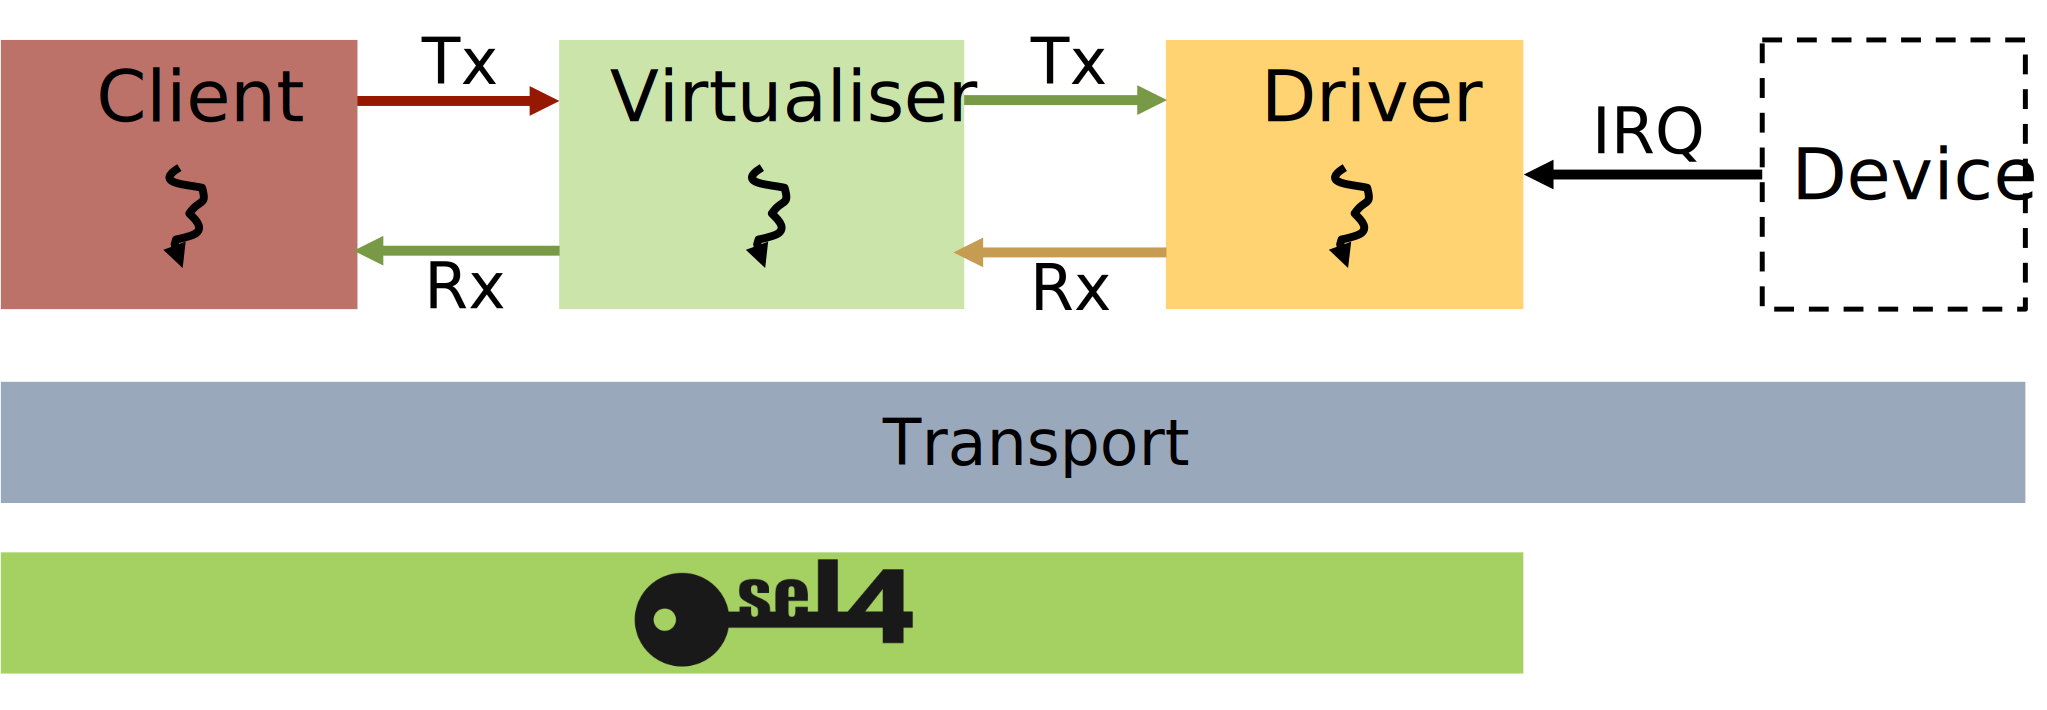
\includegraphics[scale=\figscale]{structure}
  \caption[High-level structure of I/O systems on seL4, using network
    terminology.]{High-level structure of I/O systems on seL4, using network
    terminology. Coloured boxes are software components, grey
    indicates a shared memory region.}
  \label{f:structure}
\end{figure}

\section{Overview}\label{s:dr-overview}

In our design we utilise the flexibility afforded by a clean-slate
design, where we can control the structure of the drivers as well as
their interface to the rest of the system's software.
Specifically we use this flexibility to define a
structure that eliminates unnecessary complexity in driver
implementations and thus makes it easier to write performant yet
correct drivers (with the intent to verify them eventually).

Our design is based on our prior work
\citep{Leslie_CFGGMPSEH_05}, which established that, using a zero-copy
transport layer with shared queues and asynchronous communication, usermode network
drivers can deliver performance competitive with in-kernel drivers. It also
incorporates what we have learned from the later Dingo
work~\citep{Ryzhyk_CKH_09}, which proposed a driver model for Linux
that would eliminate many common driver faults.

There are two general classes of devices that we deal with:
\begin{description}
\item[Simple devices,] such as sensors, produce or consume simple
  (typically one-word) data items, and are not shared between multiple
  clients. Some low-bandwidth communication devices also fall into
  this category. The drivers of these devices are invoked by
  \glsxtrfull{ppc} to pass data in or out (meaning they inherently use
  a \emph{passive driver thread} model, as presented in
  \autoref{s:dr-passive}).  Due to their simplicity this kind of
  devices needs no further elaboration here.  \autoref{s:sensors}
  describes such device classes.
\item[Devices that deal with bulk data,] (network, block, video, etc) use queues and
  shared data regions.  The rest of \autoref{s:driver} deals only with
  bulk-data driver interfaces.
\end{description}

\autoref{f:structure} shows the high-level logical structure of
bulk-data device
interfaces in the \gls{sddf}. Each coloured box represents a user-level
process that is encapsulated by seL4 and only able to communicate via
defined interfaces. The high-level view has three components:

\begin{description}
\item[Device driver:] Interfaces with the device hardware (\gls{nic},
  flash, ...), receives interrupts (as seL4 \Obj{notifications}), and
  transmits raw data between the device and the client;
\item[Client:] Is the producer/consumer of the \gls{io} data handled by
  the device. In many cases the ``Client'' is actually an \gls{os} server
  implementing a higher-level abstraction for applications, but this
  is not relevant to the \gls{sddf}.
\item[Virtualiser:] Allows a single device to be shared between one or
  more Clients. Where there are multiple clients, the Virtualiser presents the
  Client with an illusion of exclusively owning the device. Each
  control path has its own virtualiser (see \autoref{s:regs}).
\end{description}

The components are connected by simple control and notification
interfaces. The control interfaces refer to a metadata and data interface that is
provided by the \emph{transport layer}. The Driver- and Client-side
interfaces of the Virtualiser look almost the same, except the
Driver-side uses \gls{io}-space addresses, whereas the Client-side uses
offsets into the Data region.

The Client-Driver interface traditionally uses somewhat different
terminology for different device classes (e.g.\ network vs
storage). For now we use the terminology used for network devices,
referring to the output operation as \emph{transmit} (\gls{tx}) and the
input operation as \emph{receive} (\gls{rx}). We will discuss interfaces for
different device classes in \autoref{s:classes}.
%Besides the \gls{tx} and \gls{rx}
%channels, there is also a \emph{request} (Rq) channel, which lets the
%server request specific data from the device.

Each of the above processes (\(i\)) consists of (at least) one seL4
\emph{virtual address space} (\gls{vspace}) with access
rights defined by its \emph{capability space} (\gls{cspace}), a thread, and scheduling parameters. The
latter consist of a
priority, \(P_i\), and a (possibly null) scheduling context, \(S_i\). A
scheduling context has two relevant parameters, a \emph{budget},
\(C_i\) and a \emph{period}, \(T_i\), where \(C_i \leq T_i\).

For the rest of this document, unless explicitly stated otherwise, we
will use the term Client to refer to the whichever software is
interfacing to the driver via the virtualiser, keeping in mind that in a particular
configuration this could be a component implementing an
\gls{os} abstraction, a copier, or a directly-connected
application.

In fact, this reflects a flexibility enabled by our design based on
strict separation of concerns: components such as copiers can
be transparently added or removed depending on the requirements of the
specific system. Similarly, issues such as mapping of virtual (Client)
addresses to device \gls{io} addresses, or dynamic re-mapping of \gls{dma} regions,
are of no concern to the Driver.

\section{Transport layer}\label{s:transport}

The transport layer consists of a number of shared memory regions,
data structures in those regions, and access protocols. It is designed
to minimise software overheads by minimising (ideally eliminating)
copying of data.

\subsection{Memory regions}\label{s:regs}

\begin{figure}[th]
  \centering
  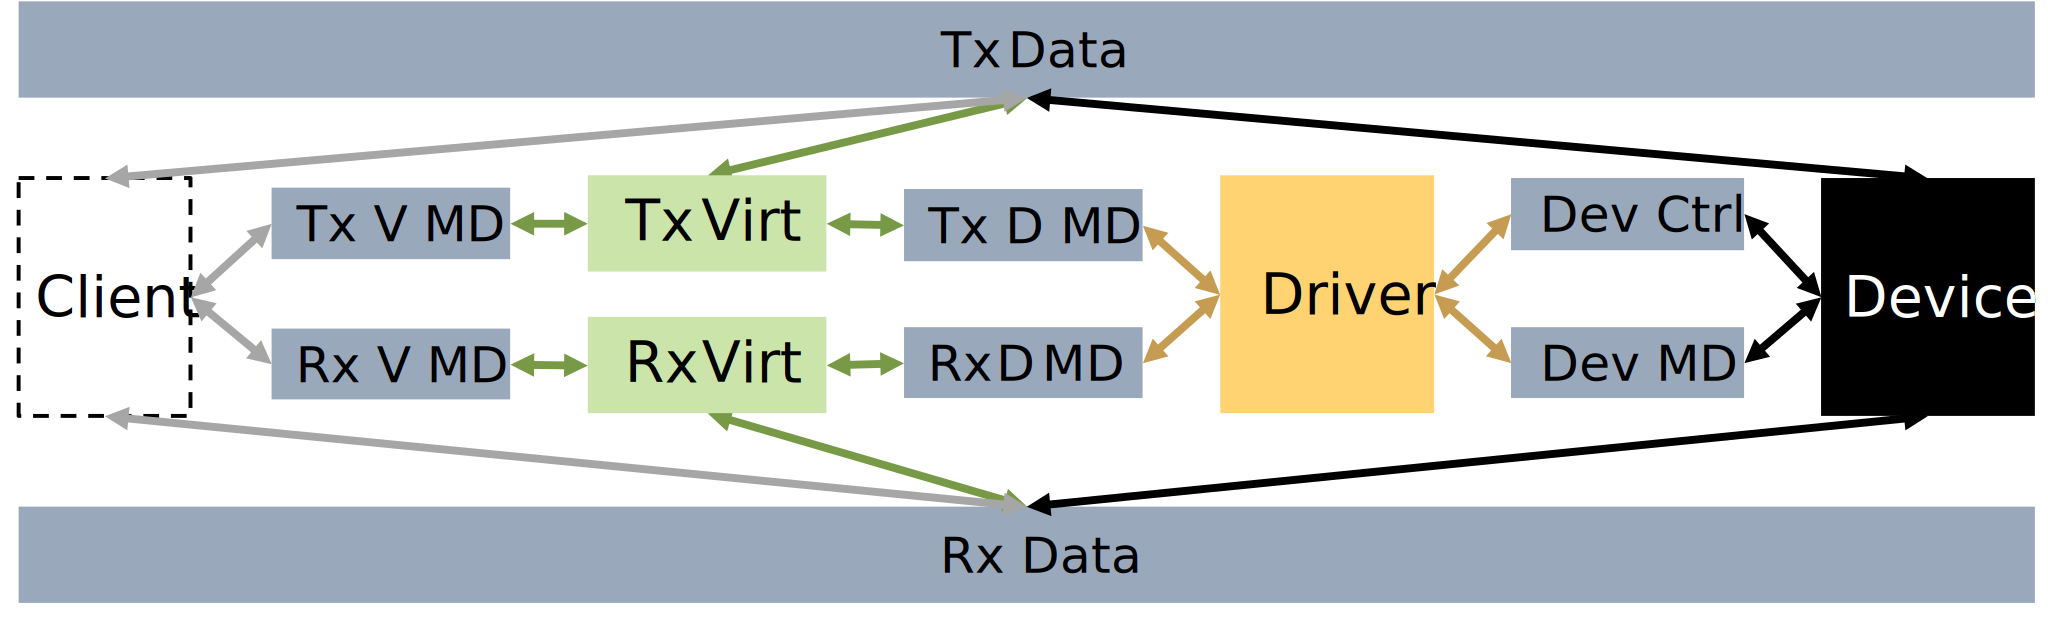
\includegraphics[scale=\figscale]{regions}
  \caption[Memory regions shared between software components
    and the device.]{Memory regions (grey) shared between software components
    and the device. ``MD'' represents metadata regions of the device
    (Dev), driver (D) and virtualisers (Virt).}
  \label{f:regions}
\end{figure}

There are three types of memory
regions, as shown in \autoref{f:regions}:
\begin{enumerate}
\item a \textbf{\Obj{device control region}} (Dev Ctrl) shared between driver and device
\item multiple \textbf{\Obj{metadata regions}} (MD) shared between driver and
  device, and similar regions shared between components
\item a \textbf{\Obj{data region}} shared between client, virtualisers and device.
\end{enumerate}

Note that while the driver holds \emph{references} into the data region, it
only passes these between the virtualiser and the device; the driver never needs to
access the actual data transferred. The data region is therefore not
mapped into the driver's address space, reducing the trust required in
the driver. The driver only needs access to the metadata region.

Also, for devices (e.g.\ networking) having separate \gls{tx} and \gls{rx} control paths, the data
region will generally be split into separate \gls{tx} and \gls{rx} regions, as
indicated in \autoref{f:regions}.

\subsubsection{Driver-device interface}

The \emph{device control region} is a set of memory-mapped device
registers used to change and inquire the device state; they constitute
the primary mechanism for software to interact with hardware. The set
of device registers, and thus the size of this region, is
hardware-defined, and typically fits on a single page. Multiple
devices may share a single page of device registers, in which case the
drivers must take care not to interfere with each other.

On architectures that do not ensure cache consistency with \gls{dma},
we map the device control region \emph{uncached}
in the driver's address space. This avoids any need for cache management
by the driver (without significant performance penalty).

For simple devices, such as serial ports, the device control region constitutes
the complete hardware-software interface. Interaction happens by the
driver reading or writing individual registers (which can be byte- or
word-size).

For devices processing bulk data, there is a \emph{metadata region}
(Dev MD), which is of flexible size but usually small (few pages), located in
RAM. It contains data structures referencing the data buffers (which
transfer the actual input or output data). Typically these are
circular queues (``ring buffers''). While the format of those data
structures is hardware-defined (part of the device protocol), their size
is usually software-defined. The driver uses the device control interface to
inform the device of the size and location of the metadata
structures.

References to the metadata region (whether passed through the
device-control interface or internal pointers in the metadata region)
are \emph{I/O space addresses}.

The device accesses the metadata region by \gls{dma}. The region is
therefore also \emph{mapped uncached} in the driver's address space,
and no cache management is required by the driver.

\subsubsection{Virtualiser-driver interface}

The driver and virtualiser interface via a separate, shared
metadata region. To distinguish it from other MD regions, we
refer to this as the \emph{driver metadata} (D MD) region.
For device classes featuring multiple
(e.g.\ \gls{tx} and \gls{rx}) virtualisers, there is a separate metadata region
for each virtualiser (\gls{tx} D MD and \gls{rx} D MD).

As a general rule, the driver metadata regions are regular memory, i.e.\
\emph{mapped cached} in the driver (as well as the virtualisers). References
into the data region from the metadata region use \emph{I/O space addresses}.

For drivers that do not do \gls{dma} (e.g. our current serial drivers), the
metadata region contains the data to be transferred; they do not have
a separate data region.

\subsubsection{Client-virtualiser interface}

This interface, the \emph{virtualiser metadata region}, again consists
of one region per virtualiser. Obviously, each client has its own
virtualiser metadata region(s). The region is
regular memory (mapped cached) and looks identical to the
driver metadata region, \emph{except} that references into the data region are
\emph{offsets relative to the start of the data region}.  Generally,
each client will have its own data region(s). It is part of
the virtualiser's job to translate the offsets into the per-client
data regions into \emph{I/O space
  addresses} for the driver, adding the offset to the corresponding
base \emph{I/O space address} of each client's data
region. At least for now we require client data regions to be
contiguous area in the physical address space.
\DEFER{Do we need non-contiguous data regions?}


\subsection{Data region}\label{s:buf-states}

The layout of the data region(s) depend on the device class. In general
it contains a set of \gls{io} buffers that are referenced by the various
metadata regions. In many cases (e.g.\
networking) the data region is simply an array of equal-sized \gls{io}
buffers.

For some device classes (e.g.\ networking) the data region can be split
into separate regions for input and output.

As mentioned above, references to the data region on the client side
of the virtualiser are represented as offsets relative to the start of
the region, while the driver side uses
\gls{io}-space addresses. Translating between those references is one of
the duties of the virtualisers.

In general, each \gls{io} buffer is in one of the following states:
\begin{enumerate}
\item\label{st:so_u}\textbf{source-owned and in use:} the buffer is not referenced by a
 \Obj{metadata region} (but referenced by source-internal data structures),
  it is waiting for, or is in the process of, being filled with data;
\item\label{st:do_i} \textbf{destination-owned and idle:} the buffer
  is referenced by a \Obj{metadata
  region}, ready to be collected by the destination, it \emph{contains valid data};
\item\label{st:do_u} \textbf{destination-owned and in use:} the buffer is not referenced by a
  \Obj{metadata region} (but referenced by destination-internal data
  structures), it may be waiting for or in the process of being
  used by the destination;
\item\label{st:so_i} \textbf{source-owned and idle:} the buffer is referenced by a \Obj{metadata
  region}, ready to be collected by the source, it \emph{contains no useful data}.
\end{enumerate}
Here ``source'' stands for the component that produces data: For output
that would be the component to the left (client side) of the region as
per \autoref{f:structure}, while ``destination'' would be the
component to the right (device side) of the region.
For input, source refers to the device-side and destination to the
client-side component.

\emph{Ownership} is the exclusive right to access a buffer, as well as
the descriptor that references it in its respective metadata region. In other
words, if a buffer is owned by a component, no other component may
access the buffer nor the queue entry that references the buffer.

For device classes that have separate input and output data regions,
a particular \gls{dma} buffer is only ever used
for either output or input: An output buffer is filled by the client,
consumed by the device, and then handed back as free
to the client.  Similarly, an
input buffer is filled by the device, consumed by the client, and eventually
returned as free to the device.

While the client may change a buffer's direction (e.g.\
receiving a packet from the network, changing some of its content and
sending it back to the network), this happens outside the
framework (and may not be advisable as it will significantly
complicate buffer management).

\subsection{Metadata regions}\label{s:ownership}\label{s:metadata}

\begin{figure}[th]
  \centering
  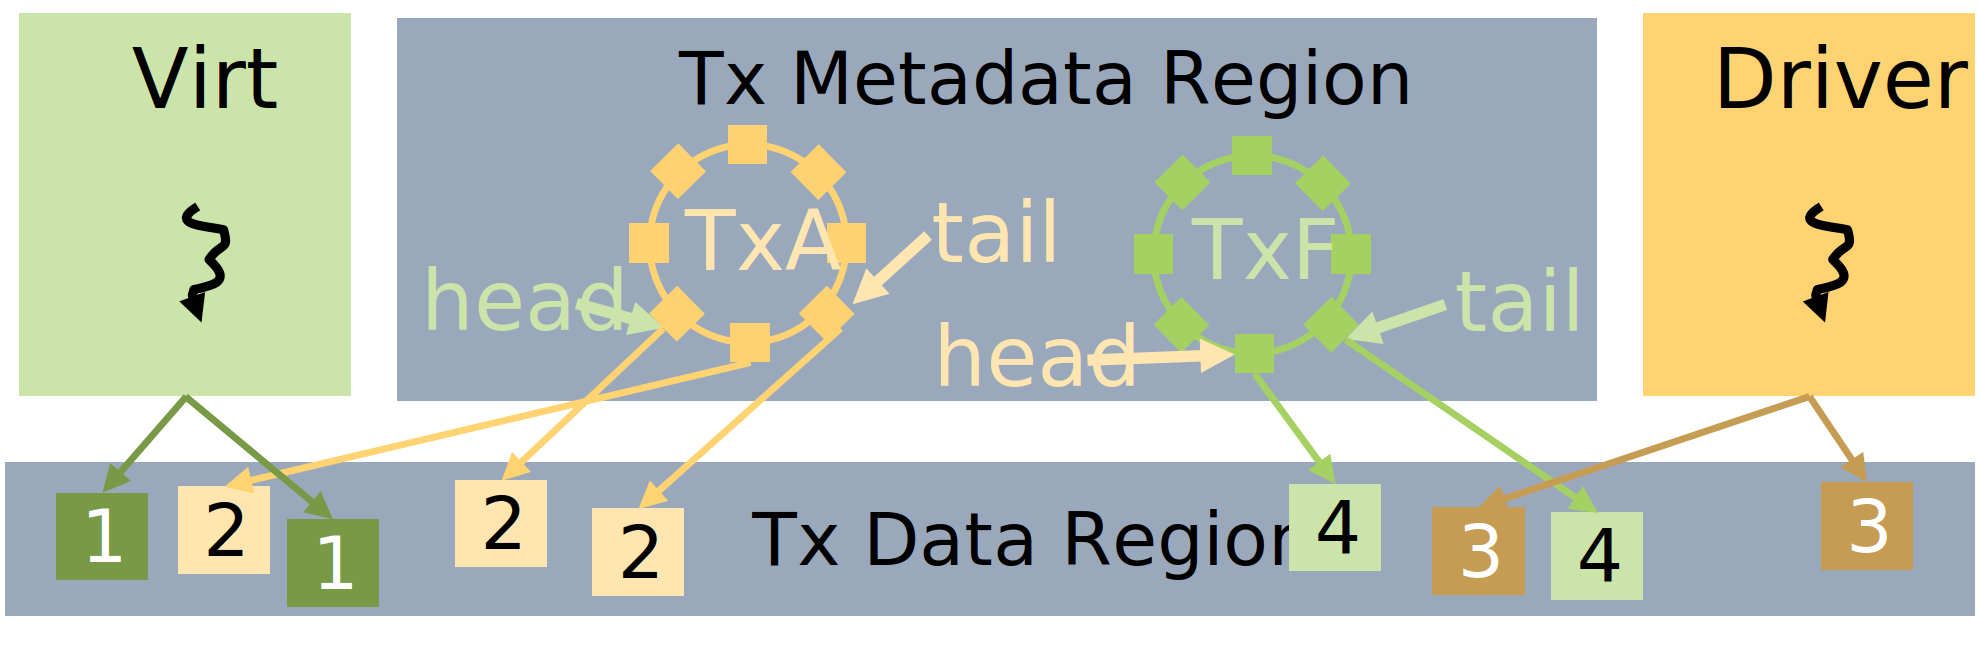
\includegraphics[scale=\figscale]{metadata}
  \caption[Tx virtualiser-driver transport layer, showing the
  \Obj{metadata} and \Obj{data regions}.]
  {Tx virtualiser-driver transport layer, showing the
    \Obj{metadata} and \Obj{data regions}. The numbers in the
    buffers in the data region indicate the buffer state as defined in
    \autoref{s:buf-states}.}
  \label{f:metadata}
\end{figure}

\autoref{f:metadata} shows the structure of the transport layer
interfacing the virtualiser and the driver, again using a \gls{tx} path as
an example.

The metadata region
uses \emph{lockless, bounded, single-producer, single-consumer queues}.
These are implemented as what is commonly referred to as ``ring
buffers''. To avoid confusion, we will not use this terminology, and
only refer to them as ``queues''. We reserve the term ``buffer'' for the
\gls{dma}-able data buffers.

The \gls{tx} metadata structure consists of two fixed-size queues, \emph{transmit
active} (\code{TxA}) of output data to be handed to the device,
and \emph{transmit free} (\code{TxF}) of buffers ready to be re-used. The \code{TxA} queue
references all buffers that are destination-owned and idle, the \code{TxF}
queue references all buffers that are source-owned and idle.

The \gls{rx} path has an equivalent structure, with two queues:
\emph{receive active} (\code{RxA}) of valid input data
to be consumed, and \emph{receive free}
(\code{RxF}) of free buffers ready to be re-used).

For a device using a request interface, there are
\emph{request active} (\code{RqA}) and \emph{request free}
(\code{RqF}) queues.

While \autoref{f:metadata} shows a driver metadata region, the virtualiser
metadata region has the same structure, the only difference being that
data region references use offsets from the start of the data area,
instead of \gls{io} addresses.

\begin{lstlisting}[gobble=2,firstline=2,float=th,tabsize=2,
  label={l:rbuf_struct},
  caption={Control region queue data structures.}]

  #define QUEUE_SIZE (1<<QUEUE_LOG_SIZE)
  struct buffer_descr {
    uint64_t io_or_offset;
    uint16_t length;
  }
  struct queue {
    uint16_t head;
    uint16_t tail;
    uint32_t consumer_signalled;
    struct buffer_descr buffers[QUEUE_SIZE];
  }
\end{lstlisting}

\autoref{l:rbuf_struct} shows the queue data structures.
Each queue has a separate \code{head} and \code{tail} index,
queue entries between those indices are valid in that they
contain an offset to a buffer in the respective data area.

Each queue has exactly one \emph{producer} and one
\emph{consumer}. Only the producer updates the tail, and
only the consumer updates the head.

Tracing the path of a \gls{tx} buffer from virtualiser to driver, the virtualiser (producer) hands
\emph{ownership} of a \gls{dma} buffer to the driver (consumer) by inserting the buffer into the \emph{active}
queue (changing its state from \circled{\ref{st:so_u}} to \circled{\ref{st:do_i}}), from where
the driver collects it (changing state from \circled{\ref{st:do_i}} to \circled{\ref{st:do_u}}). When done with a buffer,
the driver (who for this queue is the producer) hands it back to the virtualiser (now the consumer) by inserting it into the
\emph{free} queue (\circled{\ref{st:do_u}} to \circled{\ref{st:so_i}}), from where the virtualiser
can collect it (\circled{\ref{st:so_i}} to \circled{\ref{st:so_u}}).

\begin{lstlisting}[gobble=2,firstline=2,float=th,tabsize=2,
  label={l:rbuf_use},
  caption={Control-region queue management. }]

  bool empty (struct queue *queue) {
    return !((queue->tail - queue->head) % QUEUE_SIZE);
  }
  bool full (struct queue *queue) {
    return !((queue->tail + 1 - queue->head) % QUEUE_SIZE);
  }
  int enqueue(struct queue *queue, struct buffer_descr buffer) {
    if (full(queue)) return -1;
    queue->buffers[queue->tail] = buffer;
    memory_release();
    queue->tail++; (@\label{l:incr_tail}@)
    return 0;
  }
  int dequeue(struct queue *queue, struct buffer_descr *buffer) {
    if (empty(queue)) return -1;
    *buffer = queue->buffers[queue->head];
    memory_release();
    queue->head++;
    return 0;
  }
\end{lstlisting}

Specifically, as shown in \autoref{l:rbuf_use}, the producer enqueues
a data buffer at the tail by checking there is at least one unused entry,
inserting the new buffer there, and incrementing the tail pointer. Just before
updating the \code{tail} pointer, the producer issues a \emph{memory
  write barrier} to ensure that no writes are re-ordered by the compiler
or the processor across this point.
Dequeuing data buffers from the head is analogous, as per \autoref{l:rbuf_use}.

\emph{Inserting a reference to a buffer into one of the queues changes ownership} (see the
definition of buffer states in \autoref{s:buf-states}). The inserting
component loses the right to access the buffer, \emph{as well as the
descriptor referencing it}. The precise point of
ownership transfer is \autoref{l:incr_tail} in \autoref {l:rbuf_use}:
Incrementing the queue's tail pointer by the producer makes the entry
visible to the queue's consumer, which has then acquired ownership.

We can observe that ownership of data buffers is \emph{defined} by
where they are referenced: ownership of a queue entry implies
ownership of the buffer it references. An interesting consequence is
that for an active \gls{tx} buffer, ownership passes from the client to the
virtualiser, from there to the driver and from there to the
device. So, while the driver cannot access the buffer (it is not
mapped in the driver's address space) it still \emph{owns} it, for the
sole purpose of being able to pass it to the device. Hence, ownership
is a necessary but not sufficient condition for being able to access
data.

A consequence is that a buffer can at any time be referenced by at most one queue
-- this is a core integrity condition of the scheme.

Lock-free updates to these data structures are possible by
using the processor's property that \emph{reads and writes of small
integers are atomic.} The obvious data race between consumer and
producer is benign. The memory barrier is sufficient
to ensure consistency.

\subsection{Device metadata region}\label{s:dev-md}

The \Obj{device metadata region} plays a similar role in the driver-device interface
as the \Obj{driver metadata region} does in the virtualiser-driver interface.

A core difference between the two regions is that while the
\Obj{driver metadata
region} is a standard shared-memory region (shared between two
processes running on the \gls{cpu}), the \Obj{device metadata region} is a \gls{dma}
region (shared between the driver process on the \gls{cpu} and the device
hardware).

The main practical difference is that \gls{dma} bypasses the cache.  On
architectures that do not guarantee consistency between \gls{dma} and caches
(anything but Intel), this requires explicit steps to ensure
consistency. We prescribe that on such architectures \emph{the device metadata
region is mapped uncached in the driver's address space}.

\begin{lstlisting}[gobble=2,
  firstline=2,float=ht,tabsize=2,
  label={l:nic_struct},
  caption={Typical network device queue data structures.}]

  #define HW_QUEUE_SIZE (1<<HW_QUEUE_LOG_SIZE)
  struct HW_buf_descr {
    uintptr_t io_address;
    size_t    length;
    status_t  status;
  }
  struct HW_queue {
    uint32_t head;
    uint32_t tail;
    struct HW_buf_descr buffers[HW_QUEUE_SIZE];
    struct buffer_descr buffer_desc[HW_QUEUE_SIZE];
  }
\end{lstlisting}

As it interfaces with the device hardware, the \Obj{device metadata region}'s data
structures are defined by the device interface protocol (see
\autoref{s:dev_proto}). Network devices (\glspl{nic}) generally
use similar queue structures as what we specified for the \emph{driver
metadata region} in \autoref{s:metadata}
although there is usually one single queue each for transmitting and
receiving; we will call those \code{HW\_\gls{tx}} and \code{HW\_\gls{rx}},
respectively. \autoref{l:nic_struct} shows a representative example,
which we will assume for the following discussion, noting that details
may differ between devices.

Instead of separate \emph{active} and \emph{free} queues, hardware
(HW) uses the \code{status} field of each
queue entry. On output the device processes only entries marked
as \code{ready}, and, once processed, sets the \code{status} to \code{free}
or an \code{error} condition. On input, the device uses entries marked
as \code{free} and, once data is delivered, changes the \code{status} to
\code{ready} (or \code{error}). Note that the device only knows about
the location of the memory area that contains the queue; this is provided to the device via a control
register. The \code{head} and \code{tail} pointers are pure software
constructs.

\begin{lstlisting}[gobble=2,firstline=2,float=ht,tabsize=2,label={l:hw_queue_use},
  caption={Device queue management (simplified).}]

  bool HW_full (struct HW_queue *queue) {
    return (queue->head - queue->tail + 1) % HW_QUEUE_SIZE) == 0;
  }
  int HW_enqueue (struct HW_queue *queue, struct HW_buf_descr HW_buf_descr) {
    if (HW_full(queue)) return -1;
    queue->buffers[queue->tail] = HW_buf_descr;
    memory_release();
    queue->tail = (queue->tail + 1) % HW_QUEUE_SIZE;
    return 0;
  }
  int HW_dequeue (struct HW_queue *queue, struct HW_buf_descr *HW_buf_descr) {
    if (queue->buffers[queue->head].status == READY) return -1;
    *HW_buf_descr = queue->buffers[queue->head];
    memory_release();
    queue->head = (queue->head + 1) % HW_QUEUE_SIZE;
    return 0;
  }
\end{lstlisting}

\autoref{l:hw_queue_use} shows how the driver manages those
queues. For simplicity, this pseudocode assumes that the hardware processes \gls{tx} buffers
in queue order (which may not be the case in reality).

\section{Component models}\label{s:models}

\subsection{Driver}\label{s:model_driver}

The driver is event-driven, in line with conclusions
from our earlier work~\citep{Ryzhyk_CKH_09}: It acts in response to
\begin{itemize}
\item transmit requests from the virtualiser (\emph{transmit active},
  \Ta);
\item data requests from the virtualiser (\emph{data requested}, \Rq);
\item receive-ready notifications from the virtualiser (\emph{receive
    buffers free}, \Rf);
\item data-available interrupts from the device (\emph{receive
    available}, \Ra);
\item completion interrupts from the device (\emph{transmit
    completed}, \Tc).
\end{itemize}

Notwithstanding some differences in terminology, this model is a
refinement of earlier work, where we argued for \emph{active} device
drivers~\citep{Ryzhyk_ZH_10} (in the sense of having their own thread
of execution): The driver operates single-threaded in its own
address space, handling requests from either the \gls{os} (via the virtualiser) or device
interface. This model has the benefits
highlighted by \citet{Ryzhyk_ZH_10}: The driver is free
from most concurrency issues and does not need to concern itself with client
state that is not explicit in the request to be processed.

The driver thread runs at higher \emph{priority} than the
virtualiser to ensure timely handling of interrupts as well as immediate
response to virtualiser requests. Flow control (described below) prevents the driver from
monopolising the processor in the case of high incoming network load.
In the storage case, all reads are triggered (and buffers
provided) by the client (via the virtualiser) so there is no need for flow control.

\subsection{Virtualiser}\label{s:model_virt}

The virtualiser (Virt) is responsible for presenting a physical device as a
virtual device to one or more clients. Each control path (\gls{rx}/\gls{tx}/\gls{rq})
has its own virtualiser.

Virtualisation includes translating between (Client) virtual
addresses and \gls{io} space addresses seen by the device. \gls{io} space
addresses may be physical addresses, or may be translated by an
\gls{iommu}. The translation also includes a change of representation: the
client-side interface of the virtualiser uses offsets relative to the
start of a memory region as memory references, while the driver side
uses actual addresses.

If an \gls{iommu} is used, \gls{io}-space mappings may be static (defined at
build time) or dynamic (e.g.\ to dynamically make client-provided \gls{io}
buffers available to the device). If dynamic \gls{iommu} mappings are used,
managing the \gls{iommu} is the responsibility of the virtualisers. Static
mappings generally imply the need for Copier components to keep client
address spaces separated, and also imply trusting the Driver as well
as the device hardware.

\DEFER{We'll need an actual \gls{iommu} model. Best model might have \gls{io} page
  tables to be a defined subset of the VM page tables. Needs more
  design work.}


Virtualisers generally require access to the \emph{data region},
so it is mapped in their address spaces. There are two reasons:
\begin{enumerate}
\item an \gls{rx} Virt needs access to packet headers to determine
  the destination (i.e.\ the client which should receive the data);
\item On architectures that do not guarantee coherence between caches and
  \gls{dma} accesses, the virtualisers need to do cache management on the data buffers, which (on
  most architectures) requires the buffers to be mapped in its address
  space.
\end{enumerate}


On architectures that require cache management, this must happen \emph{whenever
a buffer is handed to the device} (via the driver).
Specifically, the virtualiser must \emph{invalidate} input
(i.e.\ \emph{free}) buffers before handing them to the
driver, and must \emph{flush} output (i.e.\
\emph{active}) buffers before handing them to the driver. Speculative
reads on input buffers may happen while the \gls{io} is in progress,
requiring the virtualiser to \emph{invalidate} input (i.e.\
\emph{active}) buffers again when receiving them from the
device~\citep[p.~33]{Rutland_16}.

A virtualiser that has multiple clients presents each client with the
illusion of exclusively owning the device. This requires partitioning
(for storage) or multiplexing (for network-like devices). Details are
device-specific and will generally be based on a policy.

For network devices, the \gls{rx} Virt generally does not require a specific
run-time policy, other than the use-case independent policy of
dropping incoming packets if the \gls{rx}A queue is full. (But note that the
size of the \gls{rx} queues in the virtualiser metadata region limits the
number of \gls{rx} buffers a client can have, and thus their size enforces a
policy on the amount of \gls{rx} traffic processed for the particular
client.)

\DEFER{The copier effectively doubles the client's queue size, which
  gets in the way of rate limiting? Needs more investigation.}

\iffalse
 \courtney{Although limiting size of the active queue for a client from the
 virtualiser does limit the amount of \gls{rx} traffic the virtualiser can provide
 the client per run of execution, there are many more factors at play here.
 Above you note that the size of the copy-client queue effectively doubles
 the client's queue size... But I just wanted to point out that rate
 limiting the client is more complicated than that. We are also able to
 limit the size of the queue between the client and copier too, which could
 potentially be a better way of rate limiting the client than reducing the
 size of the copy-virtualiser queue. Without further experimentation it is
 hard to know. Given that even at maximum throughputs I have very rarely
 seen a component process more than 50 packets at a time,  while most shared
 queues have >= 512 entries, my intuition is that it would be more effective
 to rate limit a client by limiting the budget of either the client or the
 client's copier component. Limiting the copier component's budget allows
 us to reduce the rate of incoming packets without stopping the client
 from doing other important work.}
\fi

A network \gls{tx} Virt imposes some form of traffic-shaping policy, such as
priority, round-robin or bandwidth limits. Furthermore, in the \gls{tx}
path, an \gls{io} buffer is permanently associated with a particular
client: once the data is transmitted, the virtualiser will return the
buffer to the client that had originally supplied it.

\iffalse
The virtualiser, like the driver, is event-based. The \gls{tx} Virt responds to:
\begin{itemize}
\item \emph{\gls{tx}A not empty} notifications (i.e.\ data available) from the client;
\item \emph{\gls{tx}F not full} notifications (i.e.\ can receive free buffers) from the client;
\item \emph{\gls{tx}A not full} notifications (i.e.\ can receive active buffers) from the driver;
\item \emph{\gls{tx}F not empty} notifications (i.e.\ returning free buffers) from the driver.
\end{itemize}

\courtney{This is not quite right, and something that we discussed that
we would look into in the future, but does not reflect the current
protocol. The tx virt only receives \emph{two types} of notifications.
When the client has enqueued packets in their \gls{tx}A queue and when the
corresponding consumer signaled flag for that queue is not set, and
when the driver has enqueued free buffers the \gls{tx}F queue, and when
the when the corresponding consumer signaled flag is not set. We
will need to do further model checking and experimental work to see
how to construct a protocol with those types of notifications --- and
if it is more efficient. I think the paragraph should read as below
instead.}
\fi

\begin{itemize}
\item \emph{\gls{tx}A not empty} notifications (i.e.\ data available) from
  the client;
\item \emph{\gls{tx}F not empty} notifications (i.e.\ returning free
  buffers) from the driver.
\end{itemize}

The \gls{tx} Virt needs to transmit requests as quickly as possible, both to
provide the best service to the client as well as to return free
buffers. It therefore should run at a priority higher than the
clients. Flow control prevents the virtualiser (as well as the driver)
from monopolising the \gls{cpu}.

Further optimisations of this signalling protocol should be possible
and will be explored in the future. \DEFER{Optimise signalling
  protocol further.}

\subsection{Observations}\label{s:mux}
As mentioned earlier, \gls{iommu} management and cache maintenance is no concern of the
driver, it is the responsibility of the virtualiser.
Other than that,
a virtualiser does little more than moving buffer references between
queues.  A
\gls{tx} or \gls{rq} Virt will generally implement some traffic-shaping policy
(while an \gls{rx} Virt is usually policy-free).
In order to keep the implementation simple, this policy should be
tailored to the specific use case. If a different policy is needed,
the Virt should be replaced with one implementing the new policy,
rather than making it more complex.

Combining the discussion of priorities in \autoref{s:model_driver} and \autoref{s:model_virt},
we have a priority assignment of \(P_C<P_V<P_D\).
This configuration is consistent
with monolithic systems, where the \gls{os} generally runs at higher
(effective) priority than apps.
Also mentioned earlier, what we refer to as the ``client'' may in fact
be a pipeline of components, possibly comprising
copiers and a server providing an \gls{os} abstraction.  The principle of priorities increasing along
the pipeline from client to driver should also hold if the client is
in fact a pipeline of components.\footnote{This
  priority assignment is the opposite of the original device driver
  framework and addresses some of the latter's performance problems.}

Priorities may not mean much in a multicore system, where each
pair of communicating components may be located on different
cores. Hence, as in any parallel system, components \emph{must not
  make assumptions on relative execution order!} Nevertheless, to
maximise location transparency, the proposed priority assignment
should be maintained even in a multicore scenario. This will be
essential if core assignments change dynamically, e.g.\ if an
energy-management policy consolidates components in order to off-line
cores.

\section{Synchronisation}\label{s:sync}

%\subsection{Server-driver Interface}

There are two ways to implement this model: as \emph{active} or as
\emph{passive driver threads} (\autoref{f:act-pass}).  Each has some advantages and it is a-priori
not clear which one is better. We need a thorough evaluation to settle
on the preferred implementation.

\begin{figure}[th]
  \hspace*{\fill}
  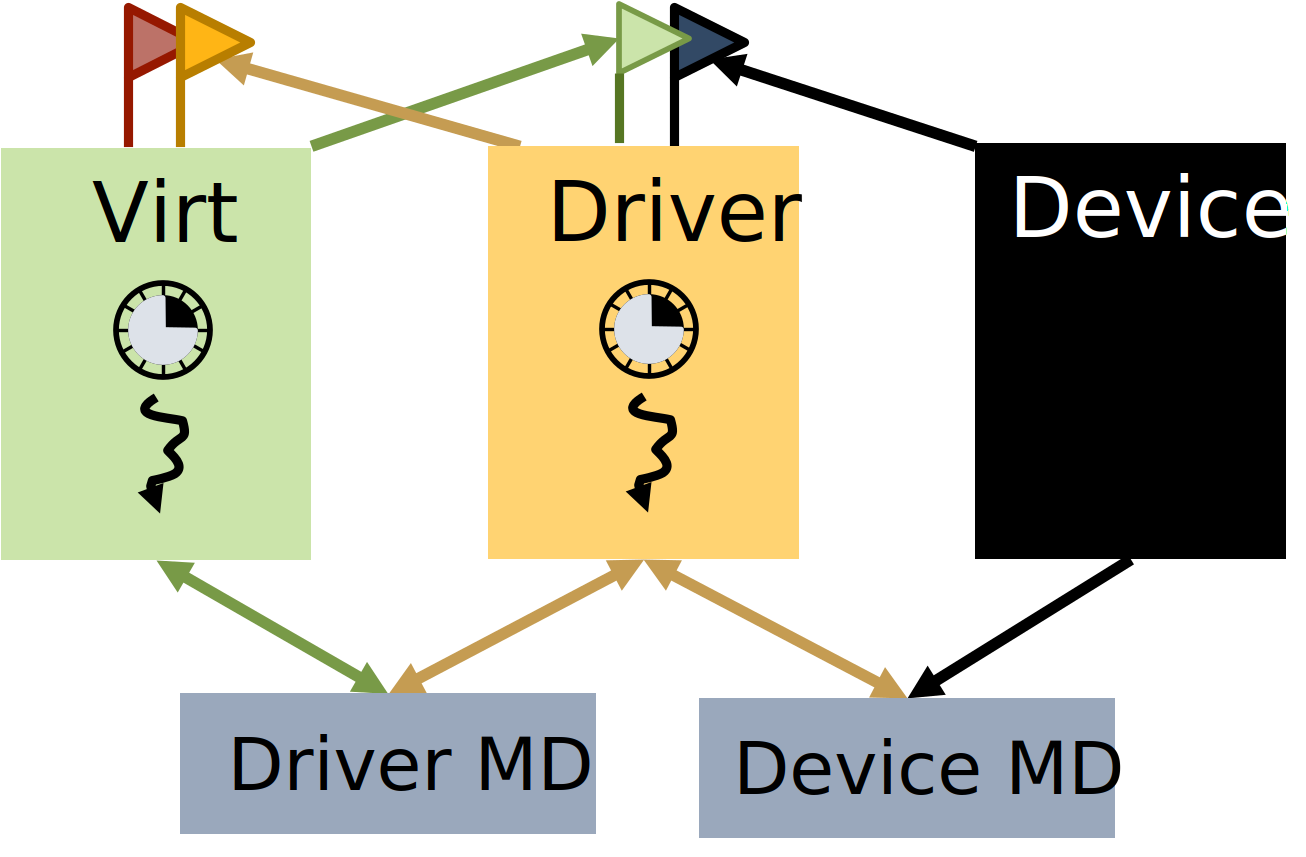
\includegraphics[scale=\figscale]{active}
  \hspace{\fill}
  \hspace{\fill}
  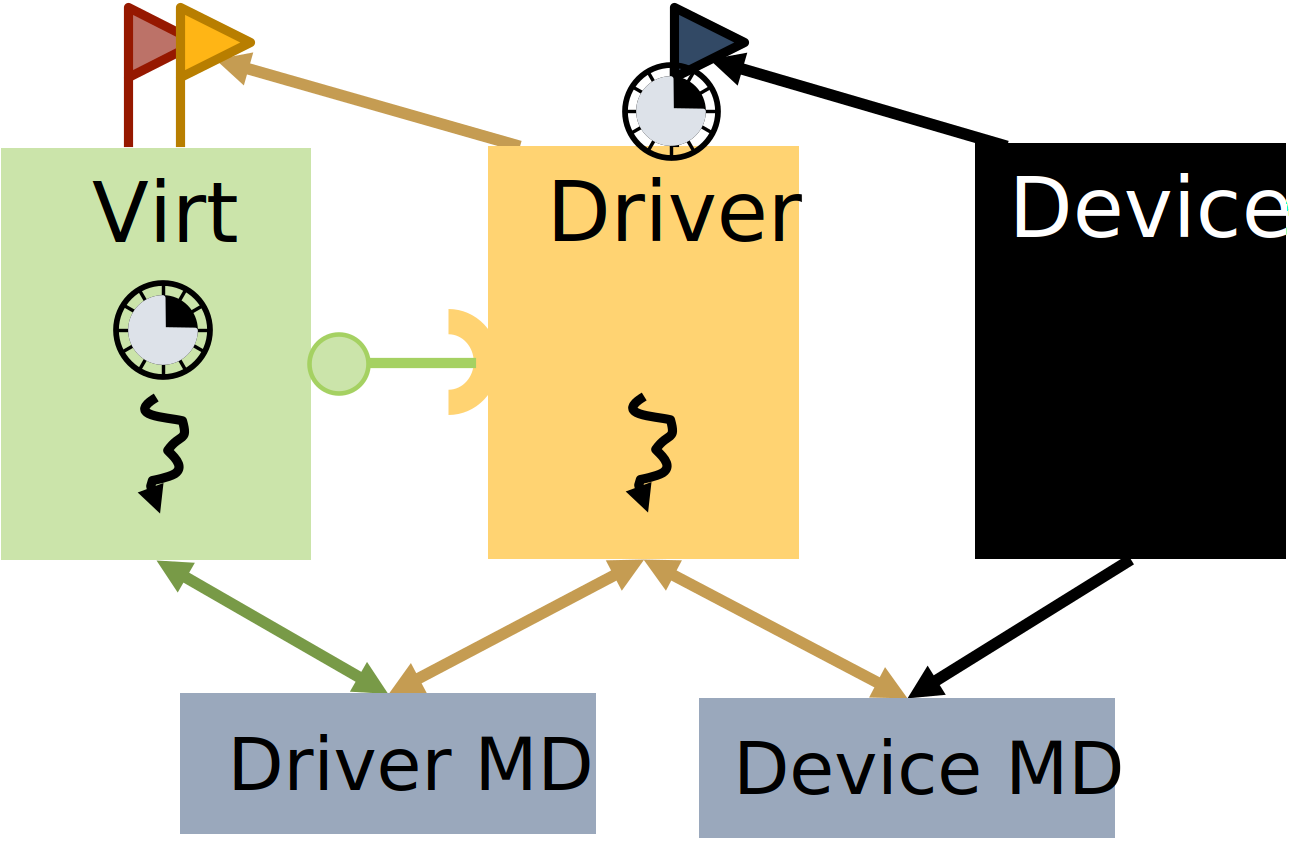
\includegraphics[scale=\figscale]{passive}
  \hspace*{\fill}
  \caption{Active (left) vs passive (right) driver-thread model.}
  \label{f:act-pass}
\end{figure}

\subsection{Active driver-thread model}\label{s:dr-active}

In this model, the driver thread is \emph{active} in seL4 MCS
terminology, meaning it has its own \emph{scheduling context}
(\gls{sc}). All its interfaces are semaphores represented by seL4
\Obj{notifications} (besides the shared memory \Obj{metadata
regions}).

More specifically, the driver and virtualiser each have a \Obj{notification}. The
virtualiser holds a badged \Obj{send} capability for the driver's \Obj{notification},
the badge identifies the virtualiser to the driver. The \gls{irq} is represented
by a different badge representing the device.

The virtualiser performs its \Ta, \Rq and \Rf operations by enqueuing
descriptors in the \Obj{driver metadata region} and signalling the
driver's \Obj{notification}. The driver uses the badge to distinguish
signals from the virtualiser and the device.

Similarly, the virtualiser has a \Obj{notification} for which the driver has a
badged capability (and the virtualiser's client holds a differently
badged capability to the same \Obj{notification}). The driver uses this
\Obj{notification}, together with a status indicator in the HW queue, to
perform the \Ra and \Tc operations.

Remember that the driver runs at higher priority than the
virtualiser. Therefore, if both components run on the same core, the
signals from the virtualiser to the driver are effectively synchronous,
resulting in an immediate context switch to the driver (unless the
driver is out of budget).

\begin{lstlisting}[gobble=2,firstline=2,float,tabsize=2,
  label={f:eth_driver},
  caption={Ethernet driver pseudocode.}]

	handle_irq() {
		while (event = clear_hw_events()) {
			if (event & Tc) {
				enqueued = false;
				while (!full(\gls{tx}F) && buf = HW_dequeue(HW_\gls{tx})) {
					enqueue(buf, \gls{tx}F);
					enqueued = true;
				}
				if (enqueued && require_signal(\gls{tx}F)) signal |= \gls{tx}F;
			}
			if (event & Ra) {
				enqueued = false;
				while (!full(\gls{rx}A) && buf = HW_dequeue(HW_\gls{rx})) {
					enqueue(buf, \gls{rx}A); /* process input */
					enqueued = true;
				}
				if (enqueued && require_signal(\gls{rx}A)) signal |= \gls{rx}A;
				while (!full(HW_\gls{rx}) && buf=dequeue(\gls{rx}F)) {
					HW_enqueue(buf, HW_\gls{rx});  /* return free \gls{rx} buffers */ (@\label{l:freeRxIRQ}@)
				}
			}
			if (event & error) {
	      		fail;
			}
		}
	}
	main() {
		initialise();
		signal = init_done;
		while (true) {
			event = signal_and_wait(signal);
			if (event & IRQ) {
				hand_irq();
				signal |= ack;
			}
			if (event & Ta) {
				while (!full(HW_\gls{tx}) && buf=dequeue(TxA)) {
					HW_enqueue(buf, HW_\gls{tx});
				}
			}
			if (event & Rf) {
				while (!full(HW_\gls{rx}) && buf=dequeue(RxF)) {
					HW_enqueue(buf, HW_\gls{rx});  /* return free Rxbuffers */  (@\label{l:freeRx}@)
				}
			}
		}
	}
\end{lstlisting}

\autoref{f:eth_driver} shows \emph{simplified} pseudocode for an Ethernet
driver.  A more optimised version will, after processing notifications
from the virtualiser, also check for pending \glspl{irq} from the device (which
may have arrived while the driver was running on behalf of the virtualisers)
and process these. Similarly, in a multicore system, virtualiser
notifications may have arrived while processing \glspl{irq} and should be
checked prior to returning. The driver will also, upon processing the
\gls{tx}-completion \gls{irq}, check whether there is work in the \gls{tx}A queue.
%\gernot{Unless the two interfaces are separate threads?}


\begin{figure}[th]
  \centering
  \hspace*{\fill}
  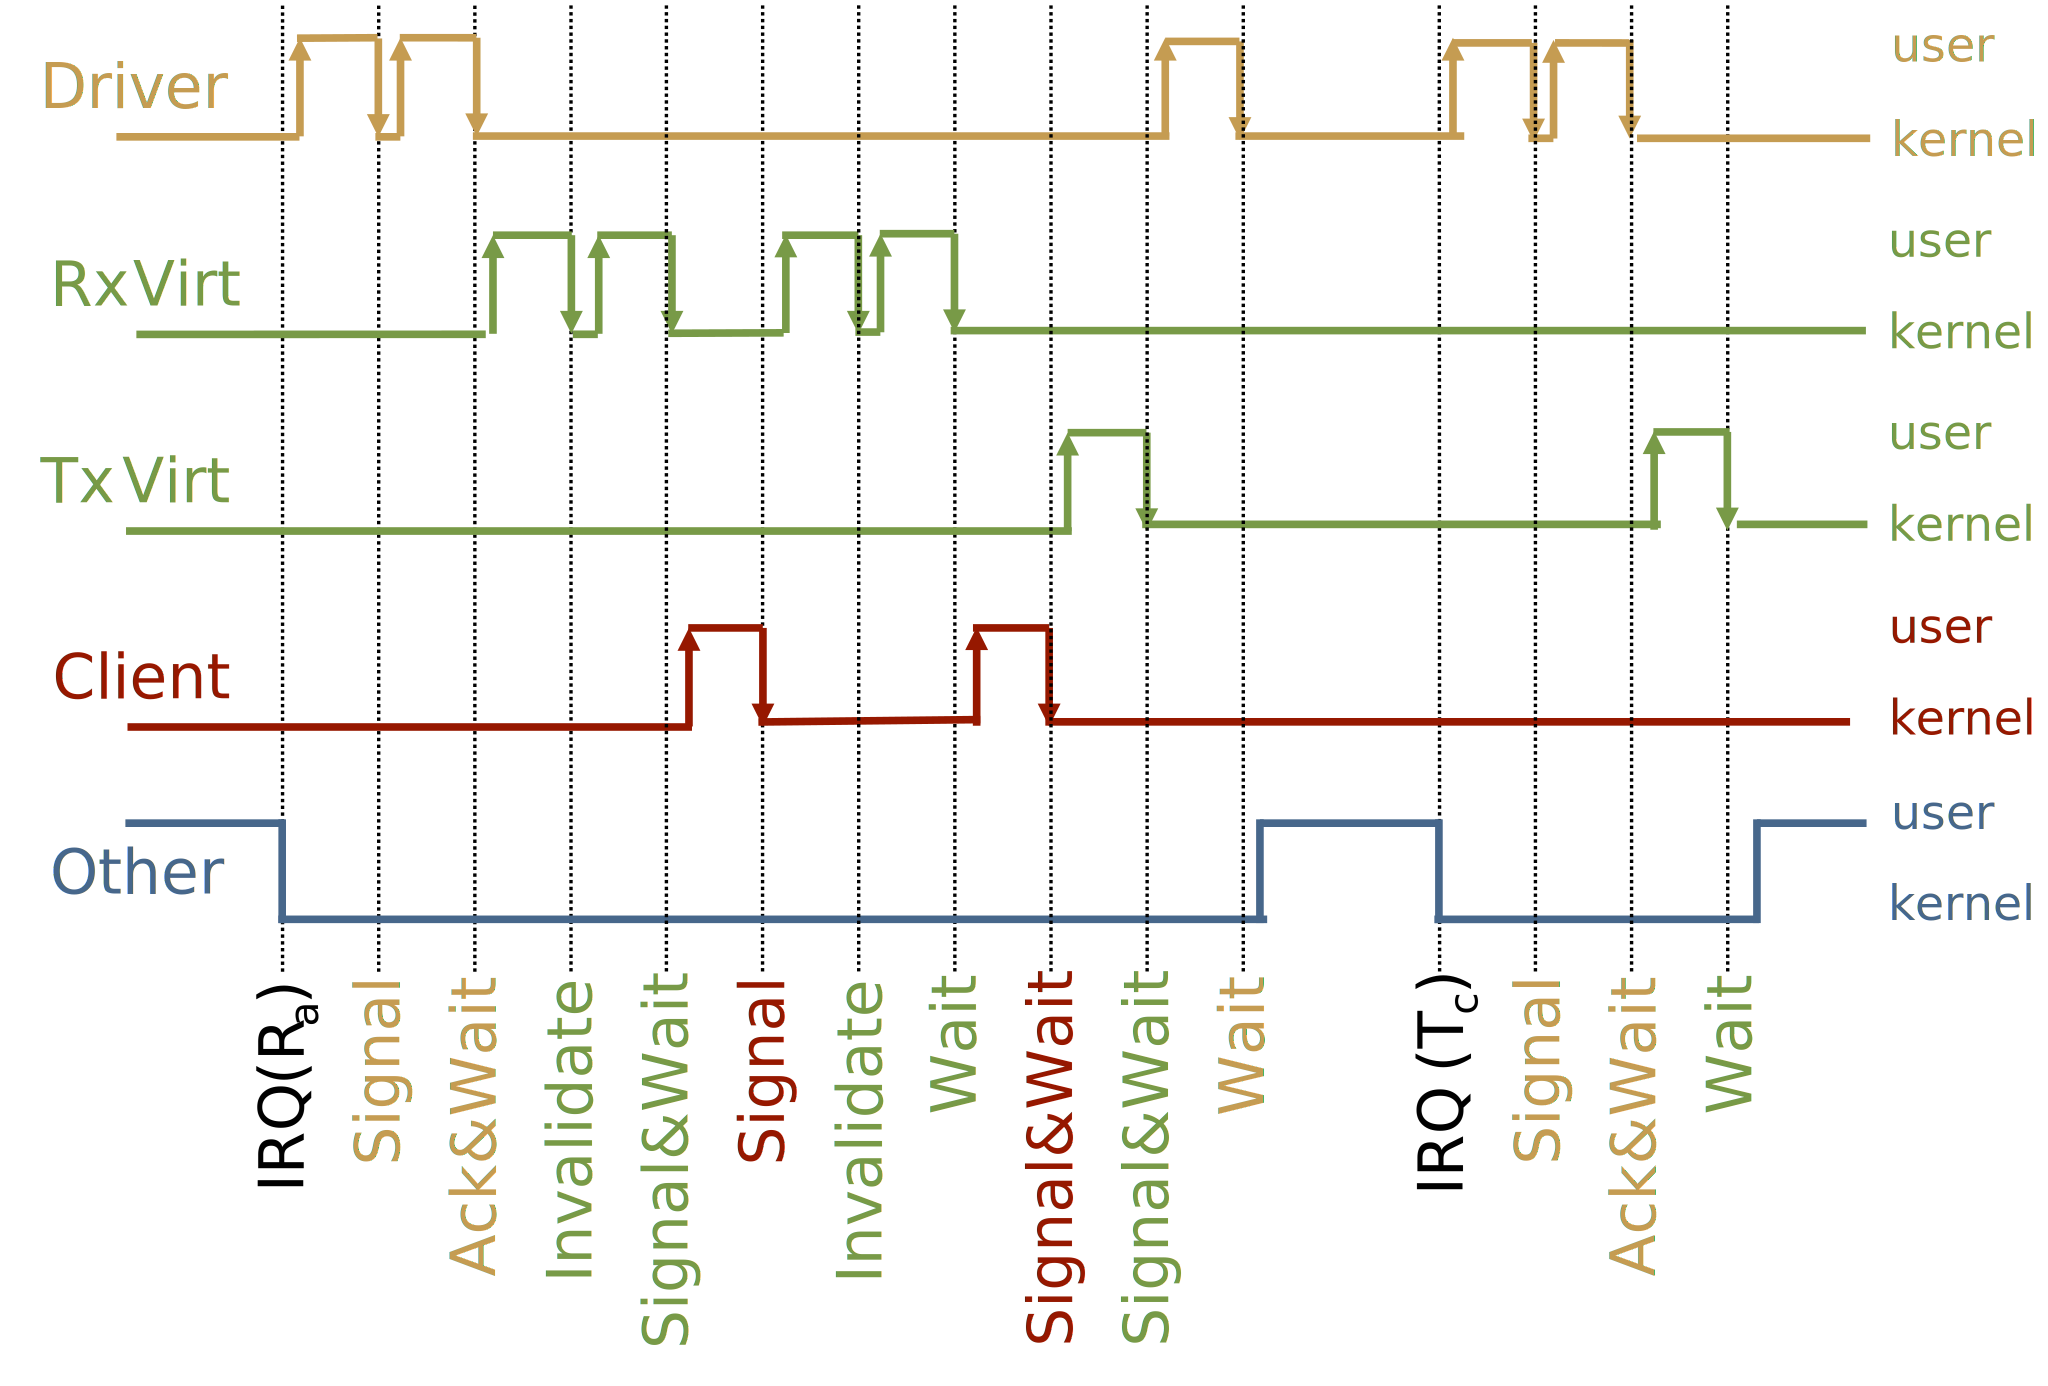
\includegraphics[scale=0.15]{entries-active}
  \hspace{\fill}
  \hspace{\fill}
  \raisebox{8mm}{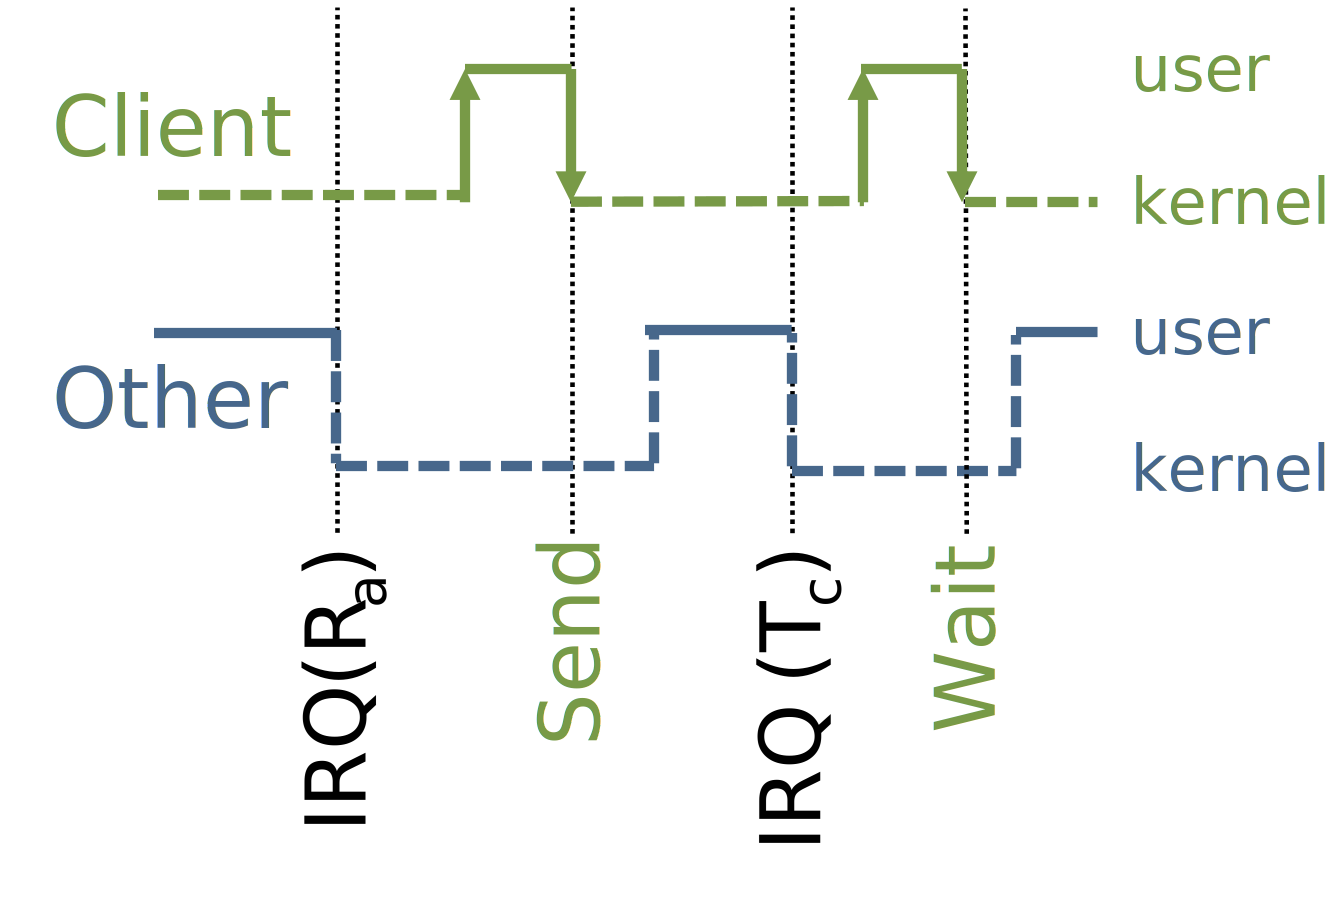
\includegraphics[scale=0.15]{entries-linux}}
  \hspace*{\fill}
  \caption[Mode switches for the active driver-thread model compared
  to Linux.]{Mode
    switches for the active driver-thread model (left) compared to
    Linux (right) for a packet round trip in a single-core setup. For horizontal lines,
    solid indicates execution, dashed indicates suspension (blocked or
    preempted). For vertical lines, arrows indicate synchronous mode
    switches (system calls and returns) while dashed lines indicate
    asynchronous switches (interrupts or scheduling). ``Other'' refers
    to a lower-priority background activity.}
  \label{f:mode-active}
\end{figure}


\autoref{f:mode-active} shows the mode switches for this model
compared to Linux.
The diagram shows a total of 15 kernel entries for a complete packet
round trip. However, if the system is under high load, it is less likely that
all signals will be required by the driver, as it is more likely that the virtualiser
is already awake and processing these queues, which is indicated to the Driver
by
% the \code{consumer\_signalled}
a flag in the respective queues.

In contrast, the Linux system only has 4 kernel entries. The
difference represents the inherent overhead of the microkernel-based
design: On Linux, each client
operation is a single system call (total 2), while in seL4 this
corresponds to context switches to the virtualisers and the driver and
back, significantly increasing the number of system
calls. Furthermore, the usermode seL4 driver requires system calls to acknowledge
\glspl{irq}. In addition, the cache management done by the virtualiser also requires
system calls, as these operations are privileged on the Arm
architecture (on RISC-V they can be delegated to usermode code,
reducing the required system calls). Linux's synchronous \gls{io} \gls{api} also avoids one kernel entry
by forcing the client to block until the send is completed, while the
\gls{sddf} \gls{api} is asynchronous (to enable execution concurrent to \gls{io}
without forcing a multi-threaded design).

Note that interrupt batching, which occurs automatically if further
interrupts arrive while the driver is processing packets with \glspl{irq}
disabled, will on average reduce the number of kernel entries per
round-trip by two for the seL4 system and by one for Linux.

Flow control is achieved by three means:
\begin{enumerate}
\item limiting the size of the receive queue in the \Obj{device metadata
  region} (which rate-limits interrupts by forcing the device to drop
  packets and thus limiting the input packet rate);
\item limiting the size of the send queue in the \Obj{driver metadata region}
  (which rate-limits the virtualiser's output requests) -- this is unlikely
  to achieve much, given that the driver runs at higher priority than
  the virtualiser;
\item limiting the driver thread's budget (which limits the amount of
  work it can do in a period, irrespective whether the work is on
  behalf of the client or to service \glspl{irq}).
\end{enumerate}

\iffalse
\gernot{I think we have now decided on more constraints on queue sizes?}
\courtney{Yes, currently \gls{sddf} queue sizes are configured so that they
each have capacity to fit all the buffers that can be enqueued in them
(i.e. they  can never be full). This does not apply to the hardware ring
sizes though, which are generally  set to be around 256 entries long,
and can therefore only fit a fraction of the total number of \gls{dma} buffers.
It would be possible to reduce or increase this size, but as you mentioned,
this doesn't tend to have much effect since the driver runs at the highest
priority.}\peterc{Same deal with virtualisers: they run at a higher
priority than the client so all their queues are always empty (except
momentarily); and there's no way for a driver to see a full queue and
stop receiving.  I believe it's possible to hammer a driver with
incoming packets so hard it spends all its time handling interrupts,
and never stops long enough for clients to process anything, as the
copy component will drop the packet after it has emptied the
virtualiser's queue ... and refilled the free queue for virtualiser
and drive} \courtney{Yes, this is actually a live lock, and I've seen it occur when I was experimenting with removing the driver's budget so it ends up spending more time handling interrupts}
%\peterc{None of this provides end-to-end flow control.  For
%  performance we want to drop unwanted packets as early as possible
%  (before doing much work on them), while allowing wanted packets
%  through.  For this to work you need some kind of feedback from the
%  clients to the driver or the first virtualiser, to drop packets
%  destined to overloaded clients} \gernot{I'm not convinced we need
%  more than what we have (incl thoughtful definition of queue sizes).}
\fi

\DEFER{Need to look at how good our queuing strategy is. Play with
  small packet sizes, low-prio clients trying to overload with
  incoming traffic...}

For a \gls{nic}, the \emph{period} of the driver's \gls{sc} should be the (desired) minimal
inter-arrival rate of packets.
%\peterc{640ns for gigabit ethernet with
%  shortest-possible ethernet frames} \gernot{Why should we encourage
%  hammering the network with minimal-size frames?}
The \emph{budget} is part of flow
control. Its choice depends on a number of factors, in particular the
relative speeds of \gls{cpu} and \gls{nic}: If the \gls{cpu} is fast enough to process
packets at line speed, the budget should be large enough to process
one incoming and one outgoing packet. If the \gls{cpu} is not fast enough,
the budget may need to be reduced to allow the back-end to keep up
with \gls{io}.

If the driver's budget is depleted, the driver is suspended by the
kernel until its budget is replenished at the end of the period. This
suspends processing \glspl{irq} as well as virtualiser requests.

Note that on each invocation, whether on an \gls{irq} or a client request,
the driver needs to check for further events that may have happened
while it was processing the current event: \glspl{irq} may arrive at any time
and the driver must poll for pending interrupts before
returning (resulting in batching). Similarly, more client requests may arrive during driver
execution, if the driver's budget was exhausted during the processing
of an event or the virtualiser runs on a different core than the driver.

More batching can be forced by using the \gls{nic}'s \emph{\gls{irq} coalescing}
feature, i.e.\ deferring the \Tc interrupt for some amount of time or
until a certain number of transmits have been completed. This is
unlikely to provide significant benefit, at least for the 1\,Gb/s (or
less) \glspl{nic} typically used in embedded systems. It might be useful for
faster \glspl{nic}.

\iffalse
For the \Ra \gls{irq}, the budget must be sufficient to enqueue
the packet(s), notify the server, and acknowledge the \gls{irq}. Similar, the \Tc \gls{irq} needs to
have sufficient budget to update queues, notify the server and
acknowledge the \gls{irq}.

Note that \gls{irq} coalescing leads to multiple packets processed for a
single \Ra interrupt, while \gls{irq} masking leads to multiple
buffers freed for a single \Tc interrupt. The budget must allow
for that.
\fi

\subsection{Passive driver-thread model}\label{s:dr-passive}

\DEFER{To be revisited whether this model makes sense at all.}

In this model, the driver thread is \emph{passive} in seL4 MCS
terminology, meaning it does not have its own \gls{sc} and can only run on
a borrowed \gls{sc}. As it runs at higher priority than the virtualiser, this makes
the client\(\rightarrow\)virtualiser invocation synchronous if both
components share a core. This
naturally leads to the virtualiser-side interface being an \Obj{endpoint}, which
is invoked by the virtualiser as a \emph{protected procedure call}, passing the
virtualiser's \gls{sc} along for the driver to execute. Thus, \Ta, \Rq and  \Rf
are invocations of the driver's \Obj{endpoint} (with the opcode passed as an
argument), while \Ra and \Tc are returns from the \Obj{endpoint} invocation.

As the driver does not have its own \gls{sc}, its \Obj{notification} (which
delivers the \gls{irq} from the device) must be active, i.e.\ have an \gls{sc}
that is lent to the driver's thread.

\iffalse
\begin{figure}[t]
  \centering
  \hspace*{\fill}
  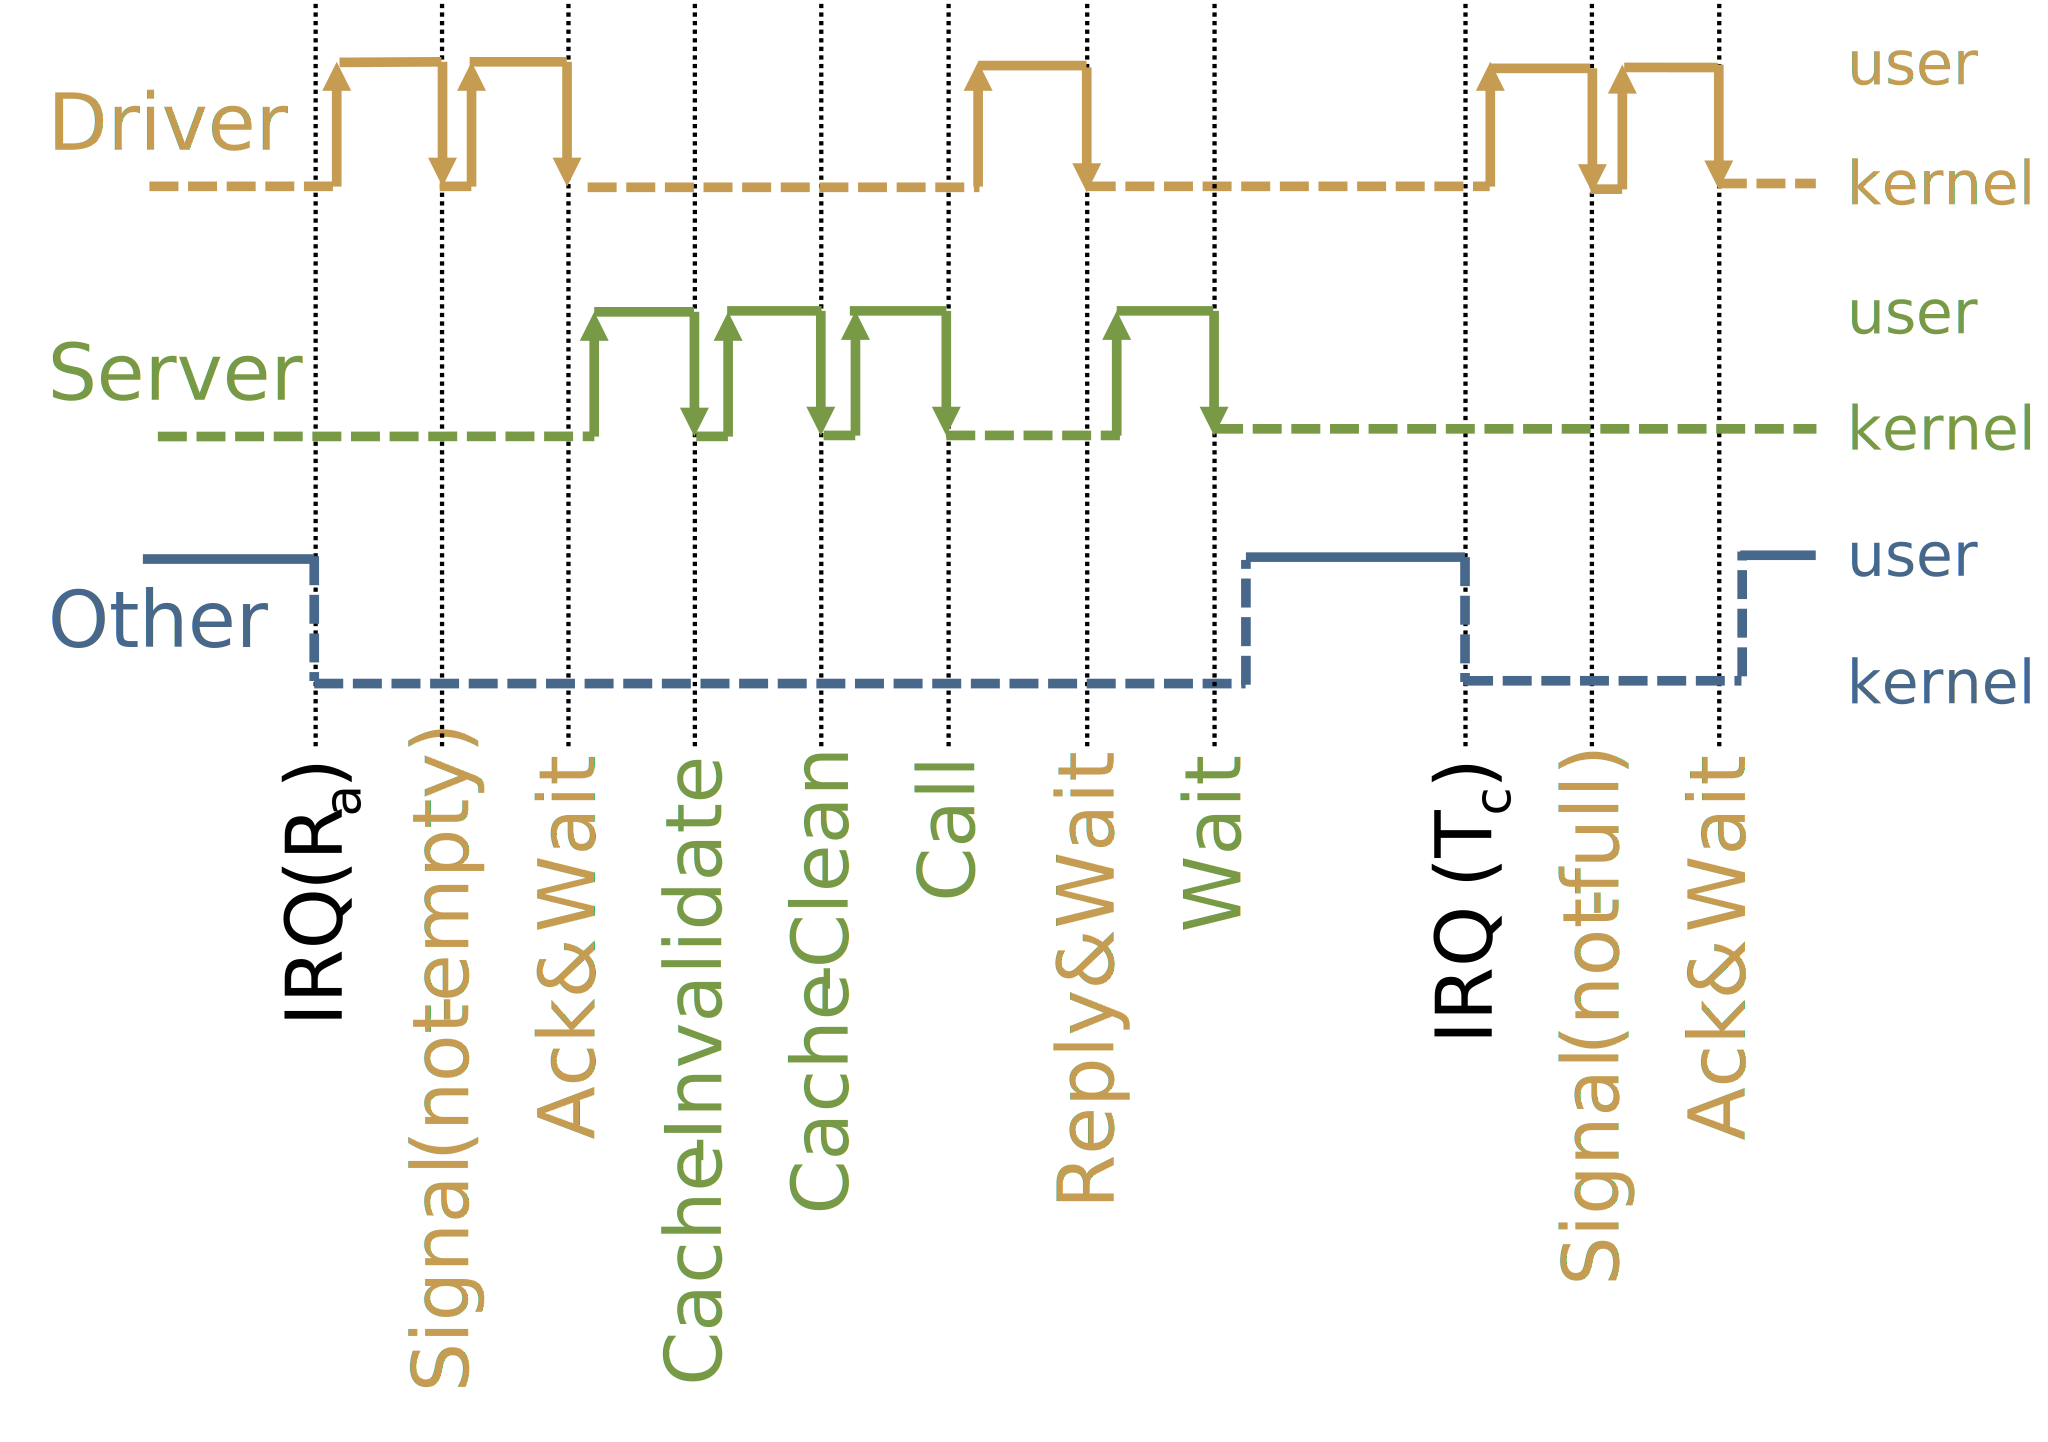
\includegraphics[scale=0.175]{entries-passive}
  \hspace{\fill}
  \hspace{\fill}
  \raisebox{17.5mm}{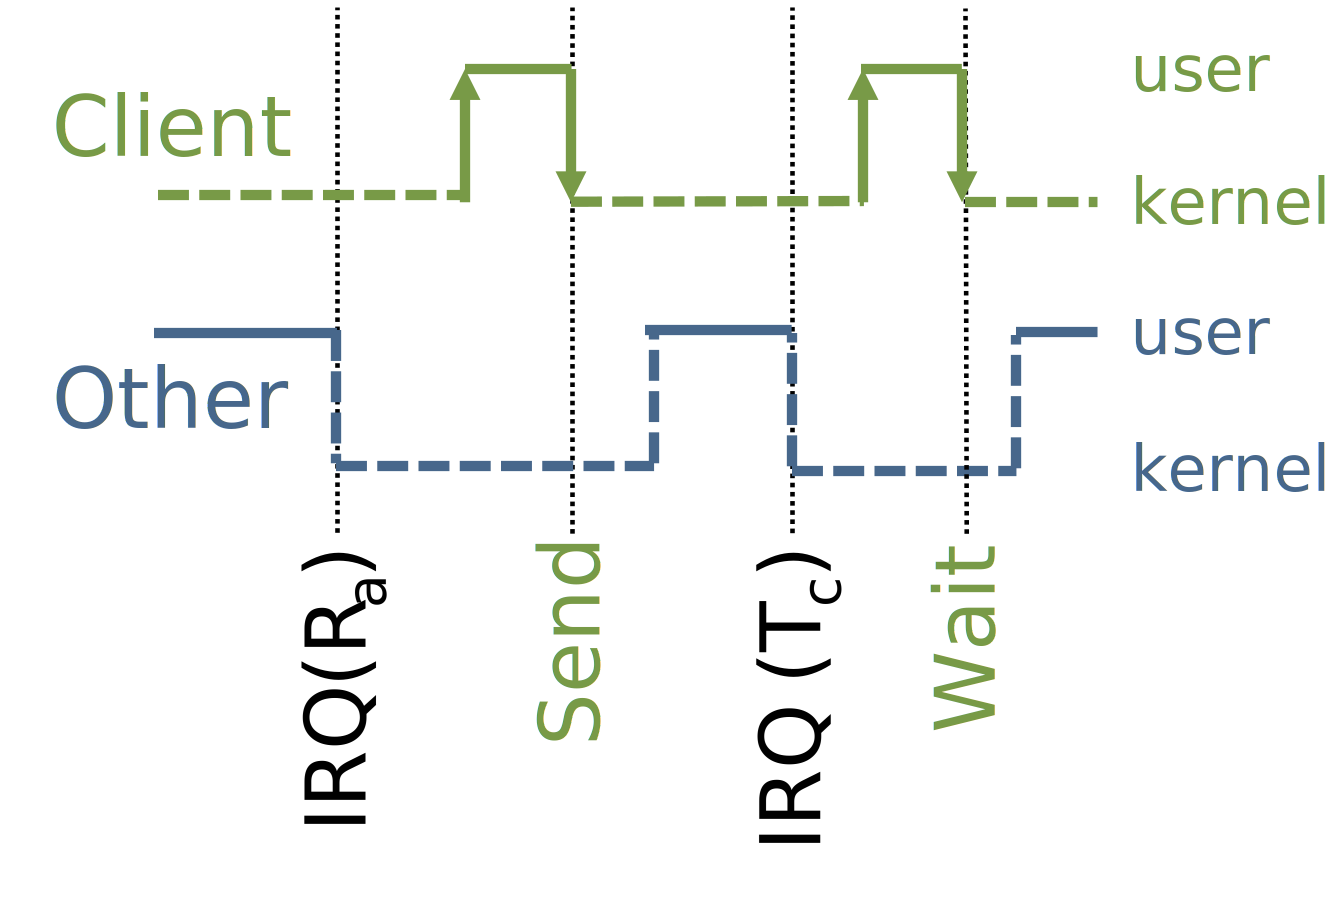
\includegraphics[scale=0.175]{entries-linux}}
  \hspace*{\fill}
  \caption[Mode switches for the passive driver-thread model compared
  to Linux.]{Mode
    switches for the passive driver-thread model (left) compared to
    Linux (right) for a packet round trip on single-core. Explanation
    as for \autoref{f:mode-active}. \TODO{FIX!}}
  \label{f:mode-passive}
\end{figure}

\autoref{f:mode-passive} shows the mode switches for the this
model. Compared to the active-thread model, there is one more mode
switch (total of 10 under low load), as the driver needs to return
control to the virtualiser after acting on the virtualiser's behalf to put a
packet on the wire. This is traded off against the virtualiser's
\code{call()} to the passive driver thread (without switching scheduling contexts)
being inherently cheaper than the virtualiser's \code{signal()} to the
higher-priority active driver thread, which requires a change in
scheduling context.
\fi

The number of mode switches in this model is similar to the active
driver model (possibly one higher). There is a performance advantage,
as a protected procedure call to a passive PD is faster than
signalling a notification to a higher-priority PD. A potential
drawback is that this forces the driver and virtualiser to be
co-located on the same core (and the virtualiser with its client, if
it is also passive). The performance trade-offs are not obvious and
need evaluation.

Flow control is achieved by three means:
\begin{enumerate}
\item limiting the size of the receive queue in the \Obj{metadata
  region};
\item limiting the size of the send queue in the \Obj{control
    region} (same caveat applies as for the active driver thread);
\item limiting the budget of the driver's \Obj{notification} (which
  implicitly limits the interrupt rate without limiting the driver's
  ability to respond to virtualiser requests, but see below for more
  detailed discussion).
\end{enumerate}

For a \gls{nic}, the period of the \Obj{Notification's} \gls{sc} should be the
(desired) minimal
inter-arrival rate of packets. The budget primarily needs to allow for \gls{irq}
handling, as requests from the virtualiser execute on the latter's budget. But
note that, even if serving a virtualiser request, the driver needs to poll
for \glspl{irq} before returning, so it may handle interrupts
on the virtualiser's \gls{sc}.

However, the virtualiser is blocked during that time, unless the driver has
a timeout exception that allows it to hand control back to the client
if the budget runs out. This would, however, complicate driver logic
(including re-introducing a degree of concurrency). On the other hand,
blocking the virtualiser while the driver is waiting for a budget
replenishment reduces the virtualiser's ability to operate concurrently.

For the \Ra \gls{irq}, the budget must be sufficient to enqueue
the packet(s), notify the virtualiser, and acknowledge the \gls{irq}. Similar, the \Tc \gls{irq} needs to
have sufficient budget to update queues, notify the virtualiser and
acknowledge the \gls{irq}.

Note that \gls{irq} coalescing leads to multiple packets processed for a
single \Ra interrupt, while \gls{irq} masking leads to multiple
buffers freed for a single \Tc interrupt. The budget must allow
for that.

\subsection{Two-component driver}

It is possible to split the driver into two separate components,
one interfacing to the virtualisers (i.e.\ handling \Ta, \Rq and \Rf events)
and one interfacing to the device (handling \glspl{irq}). This allows
serving both types of requests concurrently by running the two PDs
on different cores (and \emph{only} makes sense for this case).

The idea of a two-component driver may look like heresy in light of the discussions of
\autoref{s:model_driver}, specifically the stated goal of avoiding
error-prone concurrency control inside the driver. However, it is
actually a straightforward extension and does \emph{not} require
extra concurrency control inside the driver. The two driver components do
not access the same software-provided data structures. Specifically,
only the virtualiser-interfacing component
accesses the \code{TxA} queue of \autoref{f:metadata}, while only the
device-interfacing component accesses the \code{TxF} and \code{RxA}
queues.

The only potentially competing access to a virtualiser-side queue would be for returning free
buffers from \code{RxF} to the hardware queue. In order to avoid
explicit concurrency control and maintain the single-producer,
single-consumer property of the queues, we need to restrict accessing
this queue to the virtualiser-side component (\autoref{l:freeRx}
of \autoref{f:eth_driver}) -- the identical code in the \gls{irq} handler
(\autoref{l:freeRxIRQ} of \autoref{f:eth_driver}) is a performance
optimisation, not a functional requirement.

The performance benefit of this optimisation in the multi-component
case is not obvious without detailed evaluation. An evaluation
performed by~\citet[Sect.~7.4.3]{Parker:bsc} showed no performance
benefit (in fact, a slight performance degradation) and we therefore
do not investigate this model further for now.

\iffalse
but we note that, if needed, the loop at
\autoref{l:freeRxIRQ} can be replaced by
\begin{lstlisting}[gobble=2, numbers=none] %,firstnumber=\ref{l:free\gls{rx}IRQ}]

  if (!full(HW_\gls{rx}) && !empty(\gls{rx}F)) signal |= driver_s;
\end{lstlisting}
where \code{driver\_s} is the Notification of the server-side driver
thread. The race here is benign.

Similar arguments apply to the input control data
structures.

The model also rules out further optimisations for reducing the number
of kernel entries: The driver may check for pending interrupts after
processing server requests, or check for pending server requests
after processing interrupts (such new server requests cannot happen on
a single-core configuration).
% However, this is unlikely to be an issue
% where \gls{io} load is high enough to justify the use of multiple cores for
% the driver.
\fi

\iffalse
\subsection{Client-server interface}\label{s:sync_server}

Similar considerations apply to the server, which could be an active
or passive thread. As it executes at a lower
priority than the driver, its driver-side interface must be a
\Obj{notification}. As it executes at a higher priority than the client, the
client-side interface could be either a \Obj{notification} or an \Obj{endpoint},
with the same considerations applying as for the server-side driver
interface.

If the server is really a multiplexer, it would use the same interface
on the driver as on the client side, interposing
transparently. \autoref{f:pipeline} show an example with a multiplexer
sharing a \gls{nic} between a native client with its private IP stack and a
virtual machine, with all interfaces using similar lock-free, bounded,
single-consumer, single-producer data structures.

The control data structures for \gls{tx} and \gls{rx} flows are completely
separated. Consequently, the server could consist of two separate
threads (in fact, address spaces), which increases modularity but also
allows exploiting more parallelism, by allocating the threads to
different cores. Such a design may be particularly attractive for
servers that are multiplexers. They may apply different policies for
the \gls{tx} and \gls{rx} flows (e.g.\ copying \gls{tx} data to reduce trust in the
driver).
\iffalse
\gernot{I'm not enough of a networking
  expert to judge whether splitting the IP stack into separate \gls{tx} and
  \gls{rx} components if feasible.}
\lucy{I think it is 'possible' for at least some features but might be
  a lot of work/pain...
  I also think splitting a multiplexer into two components will mean we
  require extra protocols for a VM talking to a local client/another VM
  on the network and this might violate the simplicity principle... }

\peterc{It would work for some IP protocols, but not most of them.  TCP
  for example involves ACKS piggy-backed on received packets to say
  that a transmitted packet has been received; some protocols are
  entirely within the stack (ARP, DHCP)}
\fi
\fi

\subsection{Time-triggered architectures}

The model readily adapts to \emph{synchronous} (aka.\ \emph{time
  triggered}) architectures~\citep{Kopetz_03}, where each component
executes at a pre-determined time point, irrespective of
interrupts. In this case, none of the components signal notifications,
synchronisation is exclusively via timer signals. If a component
receives a signal, it processes its queues and then waits for the next
signal.

\subsection{Discussion}

The design currently has two major open questions that need more analysis.

\begin{Question}[Active or passive driver threads?]
\item The active \Obj{notification} for receiving \glspl{irq} arguably allows
  the budget to be adjusted to the driver's needs, but the need for
  checking for new work before returning reduces the benefit.
\item An \Obj{endpoint} results in the virtualiser being charged for the time the
  driver consumes on its behalf. However, this benefit is limited, as
  the \gls{irq} processing is still not accounted to a specific client.
\item Invoking a passive thread through an \Obj{endpoint} avoids switching the scheduling context, while
  signalling a higher-priority thread forces a switch of \gls{sc}, incurring
  higher cost. However, the active-thread design comes a the cost of one extra system call.
\item If the passive driver thread is blocked on budget replenishment, it
  blocks the virtualiser, reducing the benefits of using the budget for
  flow control.
\item On multicore, the \Obj{notification} forces the driver to run on a
  specific core, while the \Obj{endpoint} forces it to run on the virtualiser's
  core. Which model is better likely  depends on the application
  scenario.
\item The virtualiser may want to use a watchdog to prevent indefinitely
  blocking on an untrusted driver. As long as the virtualiser only
  synchronises with \Obj{notification}s, the watchdog timeout can be
  signalled to the virtualiser's \Obj{notification}, terminating the wait. If the
  virtualiser invokes the driver by IPC, then the watchdog would have to
  explicitly reset the virtualiser to abort the IPC, a somewhat more
  complicated operation.\footnote{The simpler aborting logic could be
    extended to IPC via a kernel change recently discussed: allowing
    specified signals to abort an IPC. The full implications of this
    change are not yet fully understood, so this change may or may not happen.}
\end{Question}

Similar questions arise for virtualiser threads, which may also be
 active or passive.

\begin{Question}[What are appropriate budgets for the driver (and virtualiser), and how
  are they determined?]
\item How important is the driver / \gls{irq} \Obj{notification} budget for
  rate-limiting the driver? Is limiting buffer size sufficient, in
  which case the driver could simply be given a full budget, removing
  the issue of the suspended (passive) driver blocking the virtualiser?
\item A virtualiser probably still only has small budgets, and a period
  matching that of the driver.
\end{Question}


\chapter{Device Classes}\label{s:classes}

Having described the general model of device drivers and their
interfaces, we will now refine those to specific device classes.


\section{Network}\label{s:cl-nw}

\subsection{Main properties}

Network devices are characterised by output being client-initiated
while input is spontaneous. While in practice inputs may result
from some client action (e.g.\ a request to a web or file server), this
is the result of higher level protocols that are invisible to the
driver (and device).

As such, network drivers do not have a request interface, only a
transmit and a receive interface. A typical network structure is shown
in \autoref{f:nw-pipeline}.

\begin{figure}[ht]
  \centering
  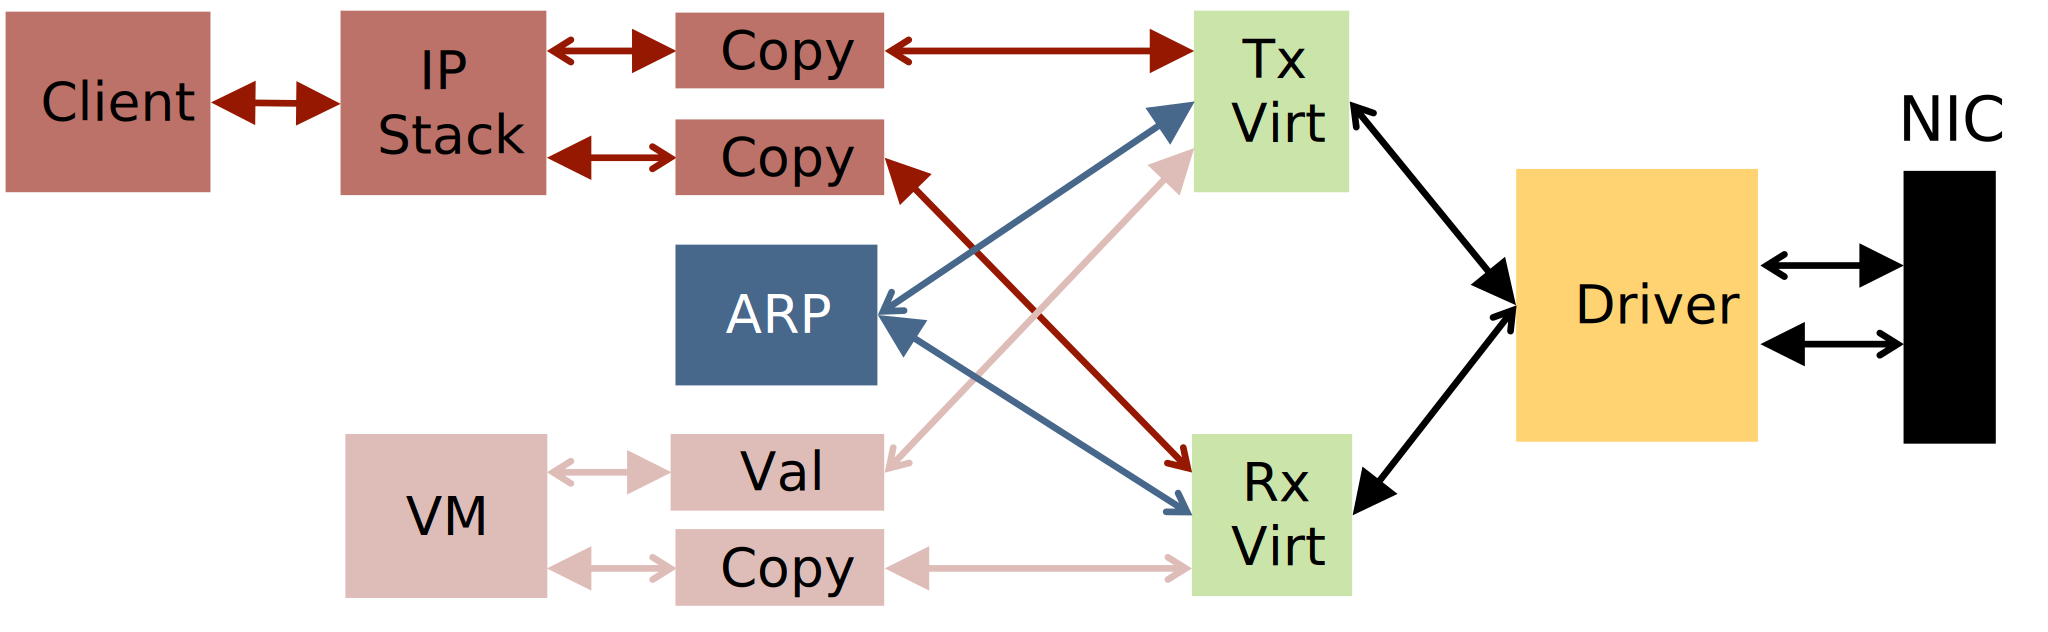
\includegraphics[width=0.9\textwidth]{pipeline-nw}
  \caption[Modularised design of a networking
  architecture.]{Modularised design of a networking architecture,
    showing
    copier (Copy) and Validator (Val) components for isolating
    untrusted clients, as well as an ARP component that handles
    broadcast requests. \FIXME{We don't need Tx-Copy and Validation is
    trivially done by the Virt.}}
  \label{f:nw-pipeline}
\end{figure}

Network devices have been our running example throughout
\autoref{s:device} and \autoref{s:driver}, so much relevant
information has already been covered. Here we summarise the main
characteristics:
\begin{itemize}
\item The  \gls{tx} and  \gls{rx} paths are separated, each with its own
  virtualiser, data region and a metadata region between any two components, as shown in \autoref{f:regions}.
\item Each of these interfaces consists of two queues. The
  \emph{active} queue (\code{TxA}/\code{RxA}) points to valid data
  buffers which the producer (Driver on input, Client on output) hands
  to the consumer.  The \emph{free} queue (\code{TxF}/\code{RxF})
  points to buffers that are returned by the consumer to the producer
  for re-use, see \autoref{f:metadata}.
\item Each \gls{io} buffer has at any time a defined \emph{owner}, and is in
  one of the four states introduced in \autoref{s:buf-states}:
  \begin{enumerate}
  \item source-owned and in use
  \item destination-owned and idle
  \item destination-owned and in use
  \item source-owned and idle.
  \end{enumerate}
\item The states are implicitly encoded in where the buffer is referenced,
  see \autoref{f:metadata}. Consequently, buffers
  change state and owners by being moved on and off the queues by
  either the producer or the consumer, see \autoref{s:ownership} for details.
\item The driver's \gls{rx} and \gls{tx} interfaces are entirely separate, in that the driver
  will only move buffers between queues of the same interface, not
  across interfaces.
\end{itemize}

\subsection{Ethernet}\label{s:cl-en}

Ethernet represents an important sub-class of network devices.
It represents a well standardised category, with common properties
such as frame size. Specifically, Ethernet devices have a standard
transfer granularity, called a \emph{frame}, of 1.5\,kB. Many Ethernet
devices also support larger frames, called \emph{jumbo frames}, but we
do not consider them here.

Server platforms frequently feature \emph{self-virtualising
  \glspl{nic}}, with multiple interfaces to the same underlying
device. These enable secure pass-through access of the same device to
multiple virtual machines.  Using this feature generally involves
extra work by the hypervisor to handle broadcast traffic. For now we
do not plan to support this feature.

\DEFER{Is wifi Ethernet-like? --- more or less, but needs extra
  level-1 management for authentication, power management, and
  roaming; plus it tends to be a lot lossier}

\subsection{Status}

The specifications for Ethernet are tested and evaluated, they are
\textbf{stable}.

\section{Serial ports}\label{s:cl-serial}

The \gls{sddf} covers only asynchronous serial \gls{io} at the moment, as
synchronous serial is not anywhere near as common.

Asynchronous serial \gls{io} is very similar to networking, in that output is
client-initiated, and input is spontaneous.  At the hardware level,
communicating terminals need to agree on bit-rate, number of bits per
character, and whether a parity bit is included.

Serial tends to be much lower bandwidth (most serial ports have a
maximum bit rate around 4Mb/s; the POSIX standard only mentions up to
32768b/s.

As such the serial framework merges the data being transferred into
the same metadata region as the queue head and tail.

Note: More \textbf{details to come}.


\section{Serial busses}\label{s:cl-bus}

\subsubsection{SPI}\label{s:cl-spi}

An SPI bus consists of one host device and N client devices; this is reflected with one driver and a
corresponding virtualiser controlling the host, and a maximum of N clients controlling their 
respective device. 

All devices share three wires: clock, MISO (client to host) and MOSI (host to client); individual 
devices are addressed by pulling down its respective CS line.
SPI allows for full-duplex communication, as MISO and MOSI are always active; however, not all bytes
are meaningful. 
The smallest unit of interaction in SPI subsystem is the command:

\begin{lstlisting}[gobble=2,firstline=2,float=th,
  label={l:SPI_command_definition},
  caption={SPI Command definition.}]

  typedef struct spi_cmd {
    /* Offset in the data region to start reading from, -1 if not reading */
    size_t read_offset;
    /* Offset in the data region to start writing from, -1 if not writing */
    size_t write_offset;
    /* Number of bytes to read and/or write, or clocks to toggle if not reading or writing;
       will be the same for reading and writing due to the full-duplex nature of the bus */
    uint16_t len;
    /* Should be true for all commands in a transaction, except for the last one */
    bool cs_active_after_cmd;
  } spi_cmd_t;

\end{lstlisting}

The clients control their respective device by enqueueing transactions, which are a sequence of
commands, where the CS line is pulled low during the entire duration. 

The SPI subsystem maps each client's data region into the driver's address space, which is referred
to by commands. 

\subsubsection{I2C host}\label{s:cl-i2c}

The \gls{i2c} device class is a multi-client serial bus that allows
clients to initiate
requests (i.e.\ acting as controllers) to a device as well as receiving a response (i.e.\
acting as targets).

\begin{figure}[th]
  \centering
  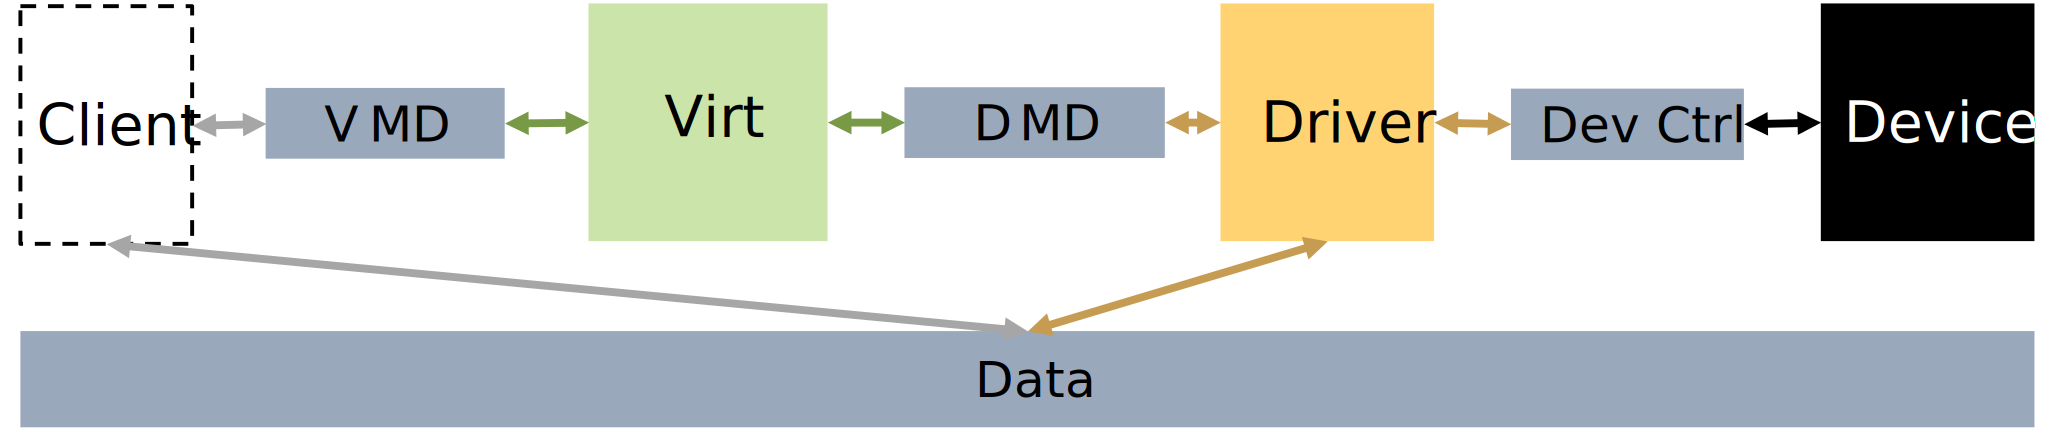
\includegraphics[scale=\figscale]{i2c}
  \caption[Memory regions shared between software components
    and the device.]{Memory regions (grey) shared between software components
    and the device. ``MD'' represents metadata regions of the driver (D) and virtualisers (V).}
  \label{f:i2c_diagram}
\end{figure}

The \gls{i2c} subsystem has each client's data region mapped directly into the driver's address space.
Each Virtualiser corresponds to exactly one driver which corresponds to exactly one \gls{i2c} bus line.
The Virtualiser checks for authentic requests before it maps client-specific offsets into a driver-specific offset and vice versa.
It also demultiplexes the responses from the driver to the correct client.
Each MD region contains only a \gls{rq} and a \gls{rs} queue.

\gls{i2c} interactions happen in terms of \emph{tokens} (1 token = 1 byte), see
\autoref{l:i2c_token_definition} for their definitions.
Intially a client will create a single request in the form of a request buffer containing tokens
and payload data which, once enqueued, travels only along the \gls{rq} interfaces between Client, Virtualiser and Driver.

\begin{lstlisting}[gobble=2,firstline=2,float=th,
  label={l:i2c_token_definition},
  caption={I2C token definitions.}]

  enum i2c_token {
    /* START: Begin a transfer. Causes master device to capture bus. */
    I2C_TOKEN_START = 0x1,
    /* ADDRESS WRITE: Address target.
    The byte immediately following this token is an integer (N) length of the
    succeeding write. Max size 255. The next N bytes are the payload. */
    I2C_TOKEN_ADDR_WRITE = 0x2,
    /* ADDRESS READ: Address target.
    The byte immediately following this token is an integer (N) length of the
    desired read. Max size 255. */
    I2C_TOKEN_ADDR_READ = 0x3,
    /* CONTINUING READ: same as ADDRESS READ, but does not end the read operation.
    Allows chaining of multiple reads for arbitrarily long read operations.
    A multi-read chain should consist of several READCs terminated by a
    final READ. */
    I2C_TOKEN_ADDR_READC = 0x4,
    /* STOP: Used to send the STOP condition on the bus to end a transaction.
    Causes master to release the bus. */
    I2C_TOKEN_STOP = 0x5,
  };
\end{lstlisting}

Note: a single I2C transaction can only be for one address.

The Driver will parse the request and potentially divide it into smaller segments,
each of which will be loaded into \gls{mmio} device registers
on an interface of an explicitly, initially configured \gls{i2c} bus line.
If the request is a READ, for each segment of the request a corresponding response
will be loaded into the \gls{mmio} device registers by the device.
The driver uses this data to build a response which re-uses the request buffer.
Once the request has been completely loaded through the registers and converted into a response,
the resulting response buffer will be enqueued by the Driver into the \gls{rs} queue.
This response now travels only along the \gls{rs} interfaces between Driver, Virtualiser and Client.

\autoref{l:i2c_queue_entry} shows the format of the entries in the \gls{rq}
and \gls{rs} queues.

\begin{lstlisting}[gobble=2,firstline=2,float=th,
  label={l:i2c_queue_entry},
  caption={I2C request and response queue entry data structure.}]

  struct i2c_queue_entry {
    size_t offset;
    unsigned int len;
    size_t bus_address;
  };
\end{lstlisting}

The Virtualiser provides a \gls{ppc} interface for a Client to claim
a free address on the \gls{i2c} bus line.

\paragraph{Status}

The basic design is \textbf{preliminary and subject to change}.

\subsubsection{USB}\label{s:cl-usb}

\ToCome{Details}

\section{Storage}\label{s:cl-storage}

\begin{figure}[th]
  \centering
  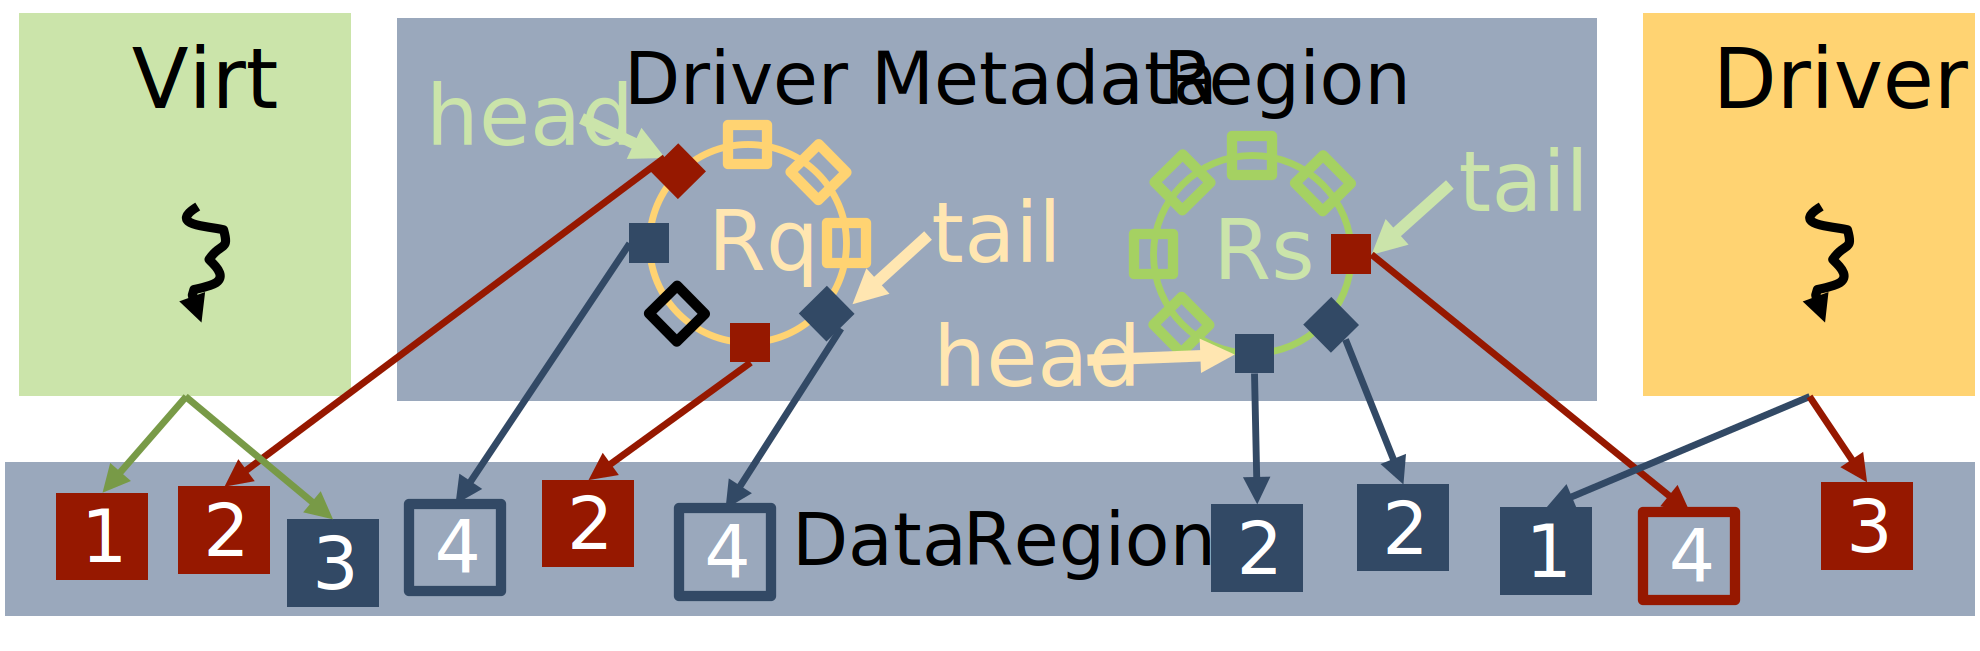
\includegraphics[scale=\figscale]{metadata-storage}
  \caption[Storage device transport layer.]{Storage device transport layer, showing the
    \Obj{control} and \Obj{data regions}. The numbers in the
    buffers in the data region indicate the buffer state, as defined
    in \autoref{s:buf-states}, where output
    buffers are red, input buffers blue. The black, empty node in the
    Rq queue indicates a \emph{barrier} request.}
  \label{f:control-storage}
\end{figure}

\subsection{Main properties}\label{s:cl-storage-props}

Storage devices deliver input upon specific requests rather than
sporadically. As such they have \emph{request} (\gls{rq}) and
\emph{response} (\gls{rs})
interfaces instead of the \gls{tx} and \gls{rx} interfaces that network devices
use. Unlike network devices there is no separation into two control
and data paths. Specifically:
\begin{itemize}
\item There is a \emph{single data region}.
\item There is a \emph{single virtualiser}.
\item  There is a \emph{single driver metadata region} that contains two queues: the \gls{rq} and
  \gls{rs} queues, as shown in \autoref{f:control-storage}.
\item The virtualiser uses the \gls{rq} queue to pass request descriptors to the
  Driver. Each descriptor holds either a \textbf{read}, a
  \textbf{write} or a \textbf{barrier} request, where read or write
  requests reference \gls{io} buffers.
\item The Driver dequeues a request from the \gls{rq} queue and (logically)
  hands it to the device.
\item Buffer states are as defined in
  \autoref{s:buf-states}.
\item Unlike for network devices, the queues reference a mixture of input
  and output buffers in arbitrary order. Inserting into the queue
  changes a buffer's state and owner. Removing from the queue changes
  the buffer's state but not the owner.
\item Specifically, the \gls{rq} queue passes buffer ownership from the
  virtualiser to the device. Until a buffer is returned in the \gls{rs} queue,
  the virtualiser (or its client) must not access it.  Buffers referenced by \textbf{write}
  requests will not be changed by the device.  Buffers referenced by
  \textbf{read} requests will be filled by the device.
  Buffer state for \emph{read} request becomes \emph{source-owned and idle} (no
  useful data in the buffer); for a \emph{write} request it becomes \emph{destination-owned
  and idle} (contains valid data).

\item Likewise, the \gls{rs} queue passes buffer ownership from the device
  to the virtualiser (and on to the client). Inserting a response into the \gls{rs} queue indicates that
  the device will not access the buffer referenced in the response.
  The buffer state is \emph{destination-owned and idle} for both read and
  write requests.
\item As the device may reorder requests, the Driver may return buffers to
  the virtualiser (via the \gls{rs} queue) in an order different from the order
  they were inserted into in the \gls{rq} queue.
\item The \textbf{barrier} request can be used to limit
  re-ordering: All requests before the barrier must be completed by
  the Driver/device before any of the requests after the barrier are
  initiated. The barrier request only ever exists in the \gls{rq} queue and
  references no buffer.
\end{itemize}

\subsection{Details}

Storage devices transfer data at the granularity of a \emph{block}.
In traditional rotating disks, this is the \emph{sector}, typically
512\,B (or a small multiple). These days, storage devices are large
and a small amount of internal fragmentation is of no
relevance. Furthermore, the setup time for a small \gls{io} operation
dominates the actual transfer time. As such, we see no benefit of
supporting such small transfer sizes, and instead specify the size of
transfers (and thus blocks) as a multiple of the platform's base page
size (usually 4\,KiB).

Where a device has an \emph{optimal transfer size} that is larger than
the page size, we use that as the block size.

Note we do not plan to support legacy devices such as \gls{cdrom}.

% Storage devices (SATA/SAS/SCSI discs, CD-roms, SPI-Rom, managed flash
% like eMMC, nvme, SD cards, or USB keys, RAM discs etc):
Our model of a storage device is thus based on the following properties:
\begin{itemize}
\item The device has a \emph{block size} that is a small integer,
  specifying the size in multiples of the
  base page size (usually the page size is 4\,KiB and the block size
  is one).
\item Large sequential (in \gls{dma} space) transfers tend to have a
  performance advantage, so the client (file server) should be able to issue
  requests larger than the block size.
\item The device may support a scatterlist of \gls{dma} blocks for output
  and this may be faster than a sequence of individual output
  requests. Hence the client should be able to issue a batch of
  requests at once.
\item The device can queue many read requests internally (typically a small power
  of two, \(2^6\cdots2^8\)).
\item Read requests can complete out-of-order (the device may re-order
  requests to increase spatial locality).
\item The device may cache write requests and perform them out-of-order
  (necessitating the use of barriers to maintain write coherence).
\item Many (but not all) storage devices are slow, so caching and
  asynchronous operation is important.
\item Solid-state storage devices wear out (they typically have
  limited write cycles). The controller transparently re-maps bad
  blocks, maintaining the illusion of a contiguous \gls{io} space. It can
  be queried in order to estimate lifetime.  Many storage devices use
  \textsc{smart}~\citep{smart:url}  for this. We plan to support a
  \textsc{smart} interface in the future.
\end{itemize}


This leads to the set of request and response structures in \autoref{l:storage_queues}.

\begin{lstlisting}[gobble=2,firstline=2,float=th,
  label={l:storage_queues},
  caption={Storage request and response queue data structures.}]

  #define QUEUE_SIZE (1<<QUEUE_LOG_SIZE)
  enum request_code {
    READ_BLOCKS,
    WRITE_BLOCKS,
    BARRIER,
    FLUSH
  };
  struct blk_request {
     enum request_code storage_command;
     uint32_t block_number;
     uint16_t count;
     void *address;
     int32_t id;
  };
  struct blk_response {
     enum {
        SUCCESS,
        /* various error codes */
     } result;
     uint16_t count;
     uint16_t success_count;
     void *address;
     int32_t id;
  };
  struct blk_req_queue {
    uint32_t head;
    uint32_t tail;
    bool     plugged;
    struct request buffer[QUEUE_SIZE];
  }
  struct blk_response_queue {
    uint32_t head;
    uint32_t tail;
    struct response buffer[QUEUE_SIZE];
  }
\end{lstlisting}

These are similar to the queues for the Ethernet devices.  The
main difference is the addition of a \code{plugged} boolean as an
optimisation.
When \code{plugged}, the driver is meant not to handle this or any
subsequent requests.  This allows the client (filesystem) to queue many requests,
up to the size of the queue, before releasing the driver to queue them
to the device.  The device then has a queue of requests it can reorder
for optimum device throughput (making use of a scatterlist if
supported by the device).  The client needs to notify the driver
when it removes the plug, in the same way it notifies the driver when
adding a request to an initially empty request queue.

The \code{id} field is to aid in matching requests and responses; it
is set by the client, maintained by the virtualiser, and copied into the response by the Driver.
This field is not strictly needed, as the request and response can
be matched on \code{address}, but may simplify the client logic.

The \code{success\_count} field in
the response structure indicates the number of
blocks successfully transferred. The \code{status} indicates the status of
the first failing transfer, or \code{SUCCESS} if all requested blocks were
transferred correctly.  Thus a request that asked for 128 blocks to be
transferred, where there was a seek error on the 67th, would return
\code{success\_count}=66, and \code{status}=\code{SEEK\_ERROR}.

In addition to the queues and shared-memory areas, there is a shared
\emph{information page} that contains the information a client might
want about a storage device, and information for monitoring the
device.  The exact layout and content is still to be determined, for
now we use the fields in \autoref{l:storage_struct}.

\begin{lstlisting}[gobble=2,firstline=2,float=th,
  label={l:storage_struct},
  caption={Storage information region data structure.}]

  struct storage_info {
     char serial_number[64];
     bool read_only;
     bool ready;
     uint16_t blocksize;
     uint16_t queue_depth;
     uint16_t cylinders, heads, blocks; /* geometry to guide FS layout */
     uint64_t size; /* number of blocksize units */
  };
\end{lstlisting}

The only non-obvious field is \code{ready}: It is initially
\code{FALSE}. The driver switches it to \code{TRUE} when the data in
\code{struct storage\_info} is valid, and the driver is
ready to accept requests.  This allows disk drives to spin up, and the
driver to query information about the attached storage, before
file systems can access the device.

The virtualiser presents a very similar interface.  We have two
virtualisers designed, and one implemented at present.

One virtualiser reads the block device's partition table, and presents
each partition on the device to a separate client.

The other lives inside a virtualiser/driver \gls{vm}, and presents a single
file on the driver's filesystem as a virtual block device to a client.

\subsection{Status}

The basic design is \textbf{stable}, but details of specifications are
\textbf{subject to change}.

\section{Sound}

\subsection{Main properties}

Sound devices expose a series of \textit{streams} each of which either
\textit{play} or \textit{record} (capture) audio. This audio is transmitted
through buffers of
\href{https://en.wikipedia.org/wiki/Pulse-code_modulation}{pulse-code
  modulation} (\gls{pcm}) frames, where
each frame contains a snapshot of the amplitude of each audio channel at a
particular point in time.

The driver exposes information about each stream to clients through shared
memory. For each stream, the driver specifies supported formats, rates, the
stream direction (playback or capture), and how many channels the stream
supports. The driver signals to the client that all streams are ready by setting
the shared \code{ready} flag to true. Until then, clients must assume no
streams are available (usually busy waiting).

Similar to storage drivers, sound drivers communicate with clients through two
pairs of request / response queues: one for commands and one for \gls{pcm} transfer.
A stream has the following life cycle:
\begin{enumerate}
  \item Take -- take ownership of the stream, specifying the number of channels, format and rate.
  \item Prepare -- allocate resources for playback.

  \textit{Client sends buffers to driver for pre-buffering.}

  \item Start -- start playback or recording.

  \textit{Driver begins responding to buffers.}

  \item Stop -- stop playback or recording.
  \item Release -- free stream resources.
\end{enumerate}

\subsection{Message Protocol}

The format of commands and \gls{pcm} requests is shown in \autoref{l:snd_command}.
The type of a command is specified by its \code{code} field, and
\code{stream\_id} denotes the stream the command refers to. The field
\code{cookie} is copied over to the corresponding response so the original
message can be identified. Commands are sent in the \code{cmd\_req} queue, and
responses are received in the \code{cmd\_res} queue.  The field \code{set\_params}
contains stream parameters for a \textit{take} request, and \code{status} is set
for responses to signal the result of a request.

To both play and record \gls{pcm} data, the client sends \gls{pcm} request through the
\code{pcm\_req} queue. The fields \code{addr} and \code{len} refer to a shared
\gls{pcm} data buffer. On playback, this buffer will contain \gls{pcm} frames to play and
on recording this buffer will be filled by the device. Once the driver has
finished with the buffer, it will respond on the \code{pcm\_res} queue updating
the \code{status} and \code{latency\_bytes}. This process differs slightly for
playback and recording.

The sound data region's ownership model is identical to Storage
(\autoref{s:cl-storage-props}), where playback is equivalent to writing and
recording is equivalent to reading.

\begin{lstlisting}[gobble=2,firstline=2,float=th,
  label={l:snd_command},
  caption={Sound definitions}]

  typedef enum {
    SOUND_CMD_TAKE,
    SOUND_CMD_PREPARE,
    SOUND_CMD_RELEASE,
    SOUND_CMD_START,
    SOUND_CMD_STOP,
  } sound_cmd_code_t;

  typedef struct sound_pcm_set_params {
    uint8_t channels;
    uint8_t format; // SOUND_PCM_FMT_*
    uint8_t rate;   // SOUND_PCM_RATE_*
  } sound_pcm_set_params_t;

  typedef struct sound_cmd {
    sound_cmd_code_t code;
    uint32_t cookie;
    uint32_t stream_id;
    union {
        sound_pcm_set_params_t set_params; // Set on TAKE request
        sound_status_t status; // Set on all responses
    };
  } sound_cmd_t;

  typedef struct sound_pcm {
    uint32_t cookie;
    uint32_t stream_id;
    uintptr_t io_or_offset;
    unsigned int len;
    // Only used in responses.
    sound_status_t status; // SOUND_S_*
    uint32_t latency_bytes; // play/record latency in bytes.
  } sound_pcm_t;
\end{lstlisting}

\subsection{Playback}

A minimal sound system consists of a \textit{client}, \textit{virtualiser}, and
\textit{driver} component, where the driver communicates to the \textit{device}
via \gls{dma}. To play audio, the client must first send \textit{take} and
\textit{prepare} commands specifying the direction as \code{SOUND\_D\_OUTPUT}
and setting stream parameters. Then, $n>0$ \gls{pcm} buffers must be pre-filled to
\code{pcm\_req} to fill the device's internal buffer, followed by a
\textit{start} command. Buffers are only responded to after they have been
played. This means the $i$th pre-filled buffer will only be responded to after
$i$ buffers have been consumed. After the stream has been started, the client
must \textbf{\textit{replay}} (send again) these $n$ pre-filled buffers. The
$i$th replayed buffer will not be responded to until $n+i$ buffers have been
played.

An example is shown in \autoref{f:snd-tx-prebuffer} with $n=5$ pre-filled
buffers. The first three pre-fill buffers fill up the device's internal buffer,
so buffers 4 \& 5 are silently ignored. After \textit{start} is sent, the driver
will initiate playback and will respond to the $i$th pre-filled buffer after $i$
buffers have been played. While this is happening, the client \textit{replays}
buffers 1-5; buffers 1-3 are silently ignored and buffers 4-5 are sent to the
device. There are several reasons for this pre-buffering behaviour.
\begin{itemize}
  \item Pre-buffering reduces the latency of playback by starting the stream
  immediately as \textit{start} is sent.

  \item The driver can choose to not support pre-buffering by simply ignoring
  all buffers sent before \textit{start}, transparent to the client.

  \item This behaviour is required for compatibility with Linux's \gls{io}
    virtualisation framework (\gls{virtio}) sound
  implementation.
\end{itemize}

\begin{figure}[th]
  \centering
  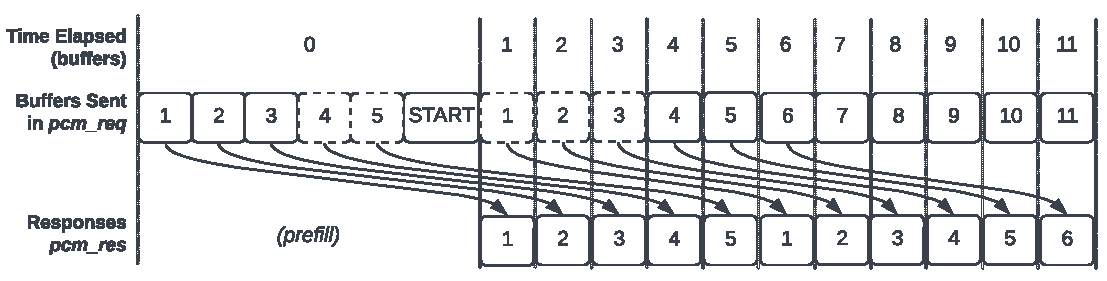
\includegraphics[width=\textwidth]{snd-tx-prebuffer}
  \caption{TX prebuffering}
  \label{f:snd-tx-prebuffer}
\end{figure}

After all \gls{pcm} buffers have been sent, the client sends a \textit{stop} command
followed by a \textit{release} command to release stream resources.

\subsection{Recording}

Recording is almost identical to playback, however there is no ``replay"
behaviour. The client first takes and prepares the stream specifying
\code{SOUND\_D\_INPUT}.  The client then pre-sends empty buffers in
\code{pcm\_req} before starting the stream. On stream start, the driver will
begin to respond to these with recorded \gls{pcm} data. The client must continue to
send empty buffers for the driver to fill. The client then sends a \textit{stop}
command and the driver fulfils the remaining requests.

\subsection{Sound Virtualisers}

The protocol is policy agnostic, however it has been designed to facilitate
various virtualiser implementations. A simple virtualiser could use the
\textit{take} and \textit{release} commands to allow clients to have temporary
exclusive ownership over a stream. If another client tries to take a stream
while it is in use, the request will fail. Alternatively, a virtualiser could
allow multiple clients to access a stream at the same time by \textit{mixing}
(combining) the audio signals.


\subsection{Status}

This device-class specification is \textbf{subject to change}.

\section{Display}\label{s:cl-display}

\ToCome{Details}

\section{Video Capture}\label{s:cl-camera}

\ToCome{Details}


\section{Pin Control}\label{s:pins}

\subsection{Terminology}
\begin{itemize}
  \item \textbf{Port:} refers to an input or output line of a logic instance in the chip
    (e.g. UART, DDR, HDMI, I2C,...). For example, a UART instance have TX and RX ports.
    Not to be confused with pad.
  \item \textbf{Pad:} refers to the physical pin on the chip package that is connected to
    the outside world.
  \item \textbf{Client device:} a peripheral device on board that needs pin control configuration.
\end{itemize}

\subsection{Main properties}
As a chip contains a limited number of pads, it is not feasable to map each
port to a separate pad. Hence, most pads are multiplexed between I/O
\emph{signals} (i.e.\ ports):  A pad
can be connected to one of multiple ports at a given point in time as appropriate for the
intended use case. These signal-to-pin and pin-to-signal options are selected by the input-output
multiplexer called a \emph{pin controller} or \emph{pinmux}. The pin controller is also used to configure other
electronic characteristics of a pin, such as drive strength, bias, etc. All of these configurations
can be programmed in software by writing to the pin controller's memory mapped registers.

\iffalse
\gernot{The rest of this section is specific to Microkit/LionsOS and do not
  belong here (or only in a much abstracted form) with details in Appendix~A1.}

Before the pin control driver is built, a Python script will read the target board's device tree
source file, extracting all the pin control settings and encodes them as binary values in an assembly
file. Then the driver is built and linked with the pinctrl data assembly file, creating a complete
pin control driver ELF image.

The pin control driver must be exclusively assigned the highest priority to ensure that it is the first
PD initialised in the system. At \code{init()} time, the driver will read the encoded pin control data and
write it into the pin control device's registers.
\else
The pin control driver as currently built relies on a prebuilt
description that says what should be inserted into each pin control
register.  We have a python program that generates such a description
from the device tree that describes the board and what is connected to
it.

The pin control driver's code must be run once before any driver that
uses the pins that it sets up.
\fi

A pin control driver is needed in two cases:
\begin{enumerate}
  \item When some devices on the board are not initialised by the bootloader.
  \item When there is a need for a device drivers to change pin
    control at run-time. For example, changing SD Card speeds on the
    Odroid-C4 involves switching a pin between a clock output and a
    GPIO input.
\end{enumerate}


\subsection{Message Protocol}

Currently, our pin control driver pipeline only supports setting the
default configuration. Dynamic reconfiguration of the pin controller
is in progress.  As such, the pin control driver has no software
interface at the moment.  \ToCome{Details}

\subsection{Status}

This device-class specification is \textbf{subject to change}.

\section{Sensors, PWM, GPIO, etc}\label{s:sensors}

These device classes are all very similar, and tend tend to be low
bandwidth --- transferring one bit to a few bytes at a time.  They
fall into the ``simple device'' category introduced in
\autoref{s:dr-overview}; rather than
using queues, the driver interfaces use \gls{ppc} to directly pass data.

\paragraph{Pulse-width-modulation (PWM)} is an output-only relatively
high-frequency signal that, if averaged, yields a low frequency (or
DC) signal.  To program, one specifies a \emph{period}, and a \emph{pulse width}
within that period --- the \emph{duty-cycle}.  By varying the
pulse width between 0 and 100\%, the average voltage at the output
varies between 0V and whatever the level `1' voltage is (typically
1.8\,V or 3.3\,V for today's SoCs).

\paragraph{General Purpose Input-Output (GPIO)} pins can be
programmed to act as input or output.  As an output, such a pin can be
set to a low or a high value; as an input it can detect whether it is
connected to a low or high voltage level.  On most SoCs, an input GPIO
can also be programmed to generate an interrupt under various
conditions. The conditions for these interrupts, and which
GPIOs can generate them, are SoC-specific.

There are other devices that have similar characteristics.

\subsection{Sensors}
Sensors --- things like tachometers for fans, temperature sensors,
voltage and current measurement etc., --- are generally read only;
some have a low repeat rate (you need to leave a specified minimum
time between readings).

Some sensors can be given set points to generate an interrupt when a
measurement crosses a threshold.

Some devices have more than one sensor controlled from the same set of
registers.

The interface for sensors therefore uses \gls{ppc}, and has the following
procedures that can be called:
\begin{description}
  \item[\texttt{get\_number\_sensors()}] returns the number of sensors
    controlled by this device.
  \item[\texttt{get\_reading(\emph{n})}] gets the current value
    measured by sensor \emph{n}.  If this function is called before a new
      reading can be obtained, it is implementation defined whether
      it returns the previous value, or an error.
  \item[\texttt{set\_threshold(\emph{n}, \emph{value},\emph{direction})}]
    \emph{direction} is one of three symbols: NONE, UP or DOWN.  When the
    sensor reading exceeds \emph{value} in that direction, a
    notification is generated to the caller.
    This procedure can fail if the driver cannot set interrupts for
    the threshhold.  If a threshhold is already set, this call
    supersedes it.  Calling with a direction of 'NONE' disables the
    notification.
\end{description}

\subsection{GPIOs}\label{s:gpio}
A General-Purpose I/O (GPIO) pin can be set to be input or
output; some GPIOs can trigger an interrupt if they are an input. In
addition some platforms allow a GPIO to be set into a high-impedance
output state, or an open-drain output state.

The sDDF uses \gls{ppc}s to configure, set, and query GPIO state.  GPIOs are
set up at build time so that each PPC channel corresponds to a
single pin.  Thus the driver knows which GPIO is being used by the
channel the PPC comes in on.

Entry points are, in general terms (the client library has not yet
been written):
\begin{description}
\item[\texttt{set\_direction()}]
  sets a GPIO as input, or output.
\item[\texttt{get\_value()}] returns 0 (low) or 1 (high) as
  the current status of the pin.
\item[\texttt{set\_value(\emph{value})}] sets the value
  (if an output) to low (0) or high (1).
\item[\texttt{configure\_irq(\emph{type})}] sets up the
  hardware to generate an interrupt from pin \emph{pin}.  The
  \emph{type} can be \texttt{rising\_edge}, \texttt{falling\_edge},
  \texttt{level\_low}, \texttt{level\_high}, or \texttt{none}, where
  \texttt{none} disables interrupts from this source.
\item[\texttt{configure(\emph{configure\_options})}] Platform
  dependent interface to set things like drive strength, pull-up or
  pull-down resistors, whether an output is open-drain, etc.
\end{description}

Some hardware may provide more options; these can be accessed
using additional hardware-specific \gls{ppc} interfaces.  The
ability to set a GPIO as an interrupt also varies between platforms;
some allow any GPIO to be used as in interrupt; others group GPIOs
into banks where each bank has a single interrupt that can be
allocated to one of the GPIOs in that bank.

At present there is no way to operate on more than one GPIO at a time.
This may be added later.

\subsection{PWM}\label{s:pwm}
For the Pulse-Width-Modulation (PWM) class there is
a single call that sets period and duty cycle.


\subsection{Status}

These device-class specifications are \textbf{subject to change}; code
implementing them has not yet been merged.

\chapter{Hotplugging}\label{s:hotplugging}

\section{Overview}

Some devices are not present for the lifetime of a system,
even in statically-architected systems such as those supported by the seL4
Microkit. Specifically, USB and PCIe and other device classes have support for ``hotplugging'',
where the physical devices can be removed or inserted whilst the system is running.
\gls{sddf} needs a framework that is device-class independent for handling
insertion and ejection events, so that drivers and clients are able to function
without data loss, crashes, or locking up the system.

Some common use cases for hotplugging include:

\begin{itemize}
  \item Inserting or removing a USB keyboard/mouse to create user input.

  \item Updating configuration files by transferring them to/from an external storage medium.

  \item Replacing a failed NVMe SSD drive (which might involve a change in partition UUIDs
        or potential system data loss).

  \item Updating a web server's hosted files without redeploying the entire system.

  \item Turning off WiFi to conserve energy, and re-enabling it on
    demand (with the consequence of having to reinitialise network stacks).
\end{itemize}

The sDDF, as presented so far, lacks sufficient mechanisms for
supporting the above use cases. In the next section we will outline
specific requirements for hotplugging, followed in
\autoref{s:hp-design} by a design that satisfies them.

\section{Requirements}

\begin{enumerate}
  \item There needs to be a way for driver and system to communicate
    insertion/ejection events:

        \begin{itemize}
          \item The driver needs a way to indicate to the system when a device has been inserted/ejected.

          \item Clients need a way to request for the device to be ejected, so the
                driver can power down (etc). Not every client is trusted, so we need
                a way to restrict these requests to certain clients.
        \end{itemize}

  \item The block virtualiser needs to be able to redo its partition-to-client
        mapping, as the partition layout may have changed when switching
        devices.

        \begin{itemize}
          \item Other device classes would need to do similar; e.g.~USB Keyboards.
          \item One should not need to rewrite the *entire* virtualiser; this
            policy should be separate from the other features of the virtualiser
            (e.g. virtual-to-physical mappings). System-specific policy should
            be easily replaceable.
        \end{itemize}

  \item Where multiple clients access a single device through a virtualiser,
        there should be a way to negotiate a ``safe'' ejection, where clients
        can save any active state and pause further activity.

        \begin{itemize}
          \item A system-specific policy must be able limit such
            pausing to prevent denial-of-service attacks from untrusted
            clients.
        \end{itemize}
\end{enumerate}

\section{Design}\label{s:hp-design}

We now show how these requirements are satisfied in sDDF. Our initial
focus will be on storage devices.

\subsection{Requirement 1: Insertion and Ejection}


\begin{figure}[th]
  \centering
  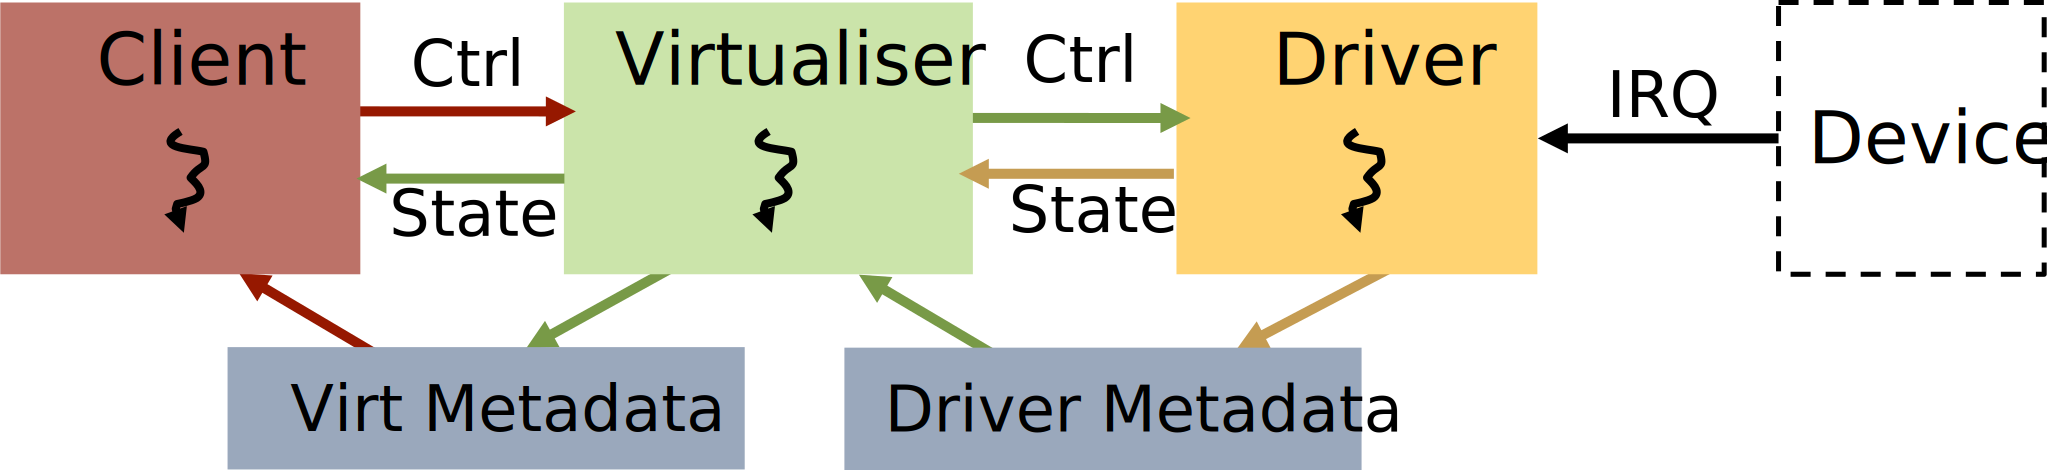
\includegraphics[scale=\figscale]{hotplug_insert_eject}
  \caption{The high-level structure of how insertion events are relayed to clients,
           and how clients can request ejection, focussed on storage devices.}
  \label{f:hotplug_insert_and_ejection}
\end{figure}

\paragraph{Driver events}

The existing block queues are not suitable for events coming from the device, as the driver can
only send responses to requests. So in the case of an insertion or
ejection, there is no way to notify clients until a request is sent,
which may never happen.

The block storage info shared page has a ready flag which could be
used, but that would require the virtualiser and clients to poll the flag.

Hence we need to add a separate notification channel, referred to as the
\emph{Block State Notification}, as this allows the driver to notify
the virtualiser on changes to the ready state.

\begin{itemize}
\item The \emph{ready} flag semantically corresponds to a readiness to
  accept block queue events.

\item This is strictly speaking, different to an inserted/ejected state,
  but ``Inserted but not ready'' is not useful.
\end{itemize}

The virtualiser is then responsible for broadcasting the driver's ready
flag to each client's ready flag, noting the following:

\begin{itemize}
\item As the \emph{Block State Notification} indicates a change, and the
  system is asynchronous, even if the client and/or virtualiser only
  sees a movement from \textbf{Ready} to \textbf{Ready} it must be
  treated as \textbf{Ready} → \textbf{Not Ready} → \textbf{Ready}.

\item When the driver becomes \textbf{Ready}, the virtualiser should
  update clients to \textbf{Ready} at the point that it has performed
  any required initialisations.
\end{itemize}


We currently implement the driver such that if the device is
physically injected or ejected, the driver begins any initialisation
or deinitialisation steps. We do not foresee the need to prevent
``auto''-insertion, downstream clients such as filesystems can
implement their own policies regarding this, but they still need to
know the device exists (and what it is).

\paragraph{Client requests}

It would be possible to extend the block request queues with
\texttt{INSERT} and \texttt{EJECT} request codes (as this flows in the
correct direction). However, this approach complicates both the
block virtualiser and the SD card driver. It would no longer be
possible to cleanly separate the initialisation phase from the
handling of client requests. Furthermore, not all device classes
support different request codes. Finally, this approach would require
the block virtualiser to implement a security policy, undermining
separation of concerns.

We instead add a small, \gls{ppc}-based control interface (see:
\texttt{include/sddf/hotplug/control.h}).  Clients can request
insertion (\texttt{REQ\_INSERT}) or ejection (\texttt{REQ\_EJECT}) and
the driver can respond indicating success (\texttt{RESP\_OK} or
\texttt{RESP\_NOOP}) or failure (\texttt{RESP\_ERROR} an insert/eject
is in progress, or \texttt{RESP\_NO\_DEV} if there is no device).

The details differ somewhat between device classes:
\begin{description}
\item[Block driver:] we re-use the \emph{Block State Notification}
  channel. We rely on restricting the channel capabilities so that
  only certain clients are able to perform \gls{ppc}s; thereby reusing
  existing security mechanisms.

\item[Other device classes:] we can re-use an appropriate channel or
  add a dedicated hotplug control \gls{ppc}.
\end{description}

\subsection{Requirement 2: Policy-free Virtualisers}

Virtualisers are responsible for taking client requests and turning them into
driver requests. In the case of the block virtualiser, each client is assigned
one partition. When the device changes, which client is assigned which partition
must also changed.

Other device classes will require similar -- network might will assign each client
a different IP address (via MAC addresses). The appropriate mappings differ
depending on the usecase of the system. Once the mappings are set up, however,
they are static, and the behaviour of the virtualiser is nearly-identical.
Keeping with our modular design, virtualisers linked against a policy library
that can be easily swapped out depending on the desired usage (or replaced
entirely).

For the block virtualiser, this resulted in the interface shown in
\autoref{l:virt_policy_protos}. This is used in an index-based static mapping
based on the MBR/GPT partition tables.

\begin{lstlisting}[gobble=2,firstline=2,float=th,tabsize=2,
  label={l:virt_policy_protos},
  caption={Virtualiser policy interface prototypes. }]

  bool virt_partitioning_init(void);

  int get_drv_block_number(uint64_t cli_block_number, uint16_t cli_count,
                           int cli_id, uint64_t *drv_block_number);

  void virt_partitioning_reset(void);
\end{lstlisting}

The \texttt{virt\_partitioning\_init\(\)} function is stateful and is called
multiple times (upon notifications) until returning true to indicate that the
policy has been initialised. This allows for the partitioning policy to send
requests to the driver if it is needed; for instance if we wanted to read the
filesystem UUIDs to map into clients. This would enable UDEV-like rules.

\subsection{Requirement 3: Safe Ejection}

\begin{figure}[th]
  \centering
  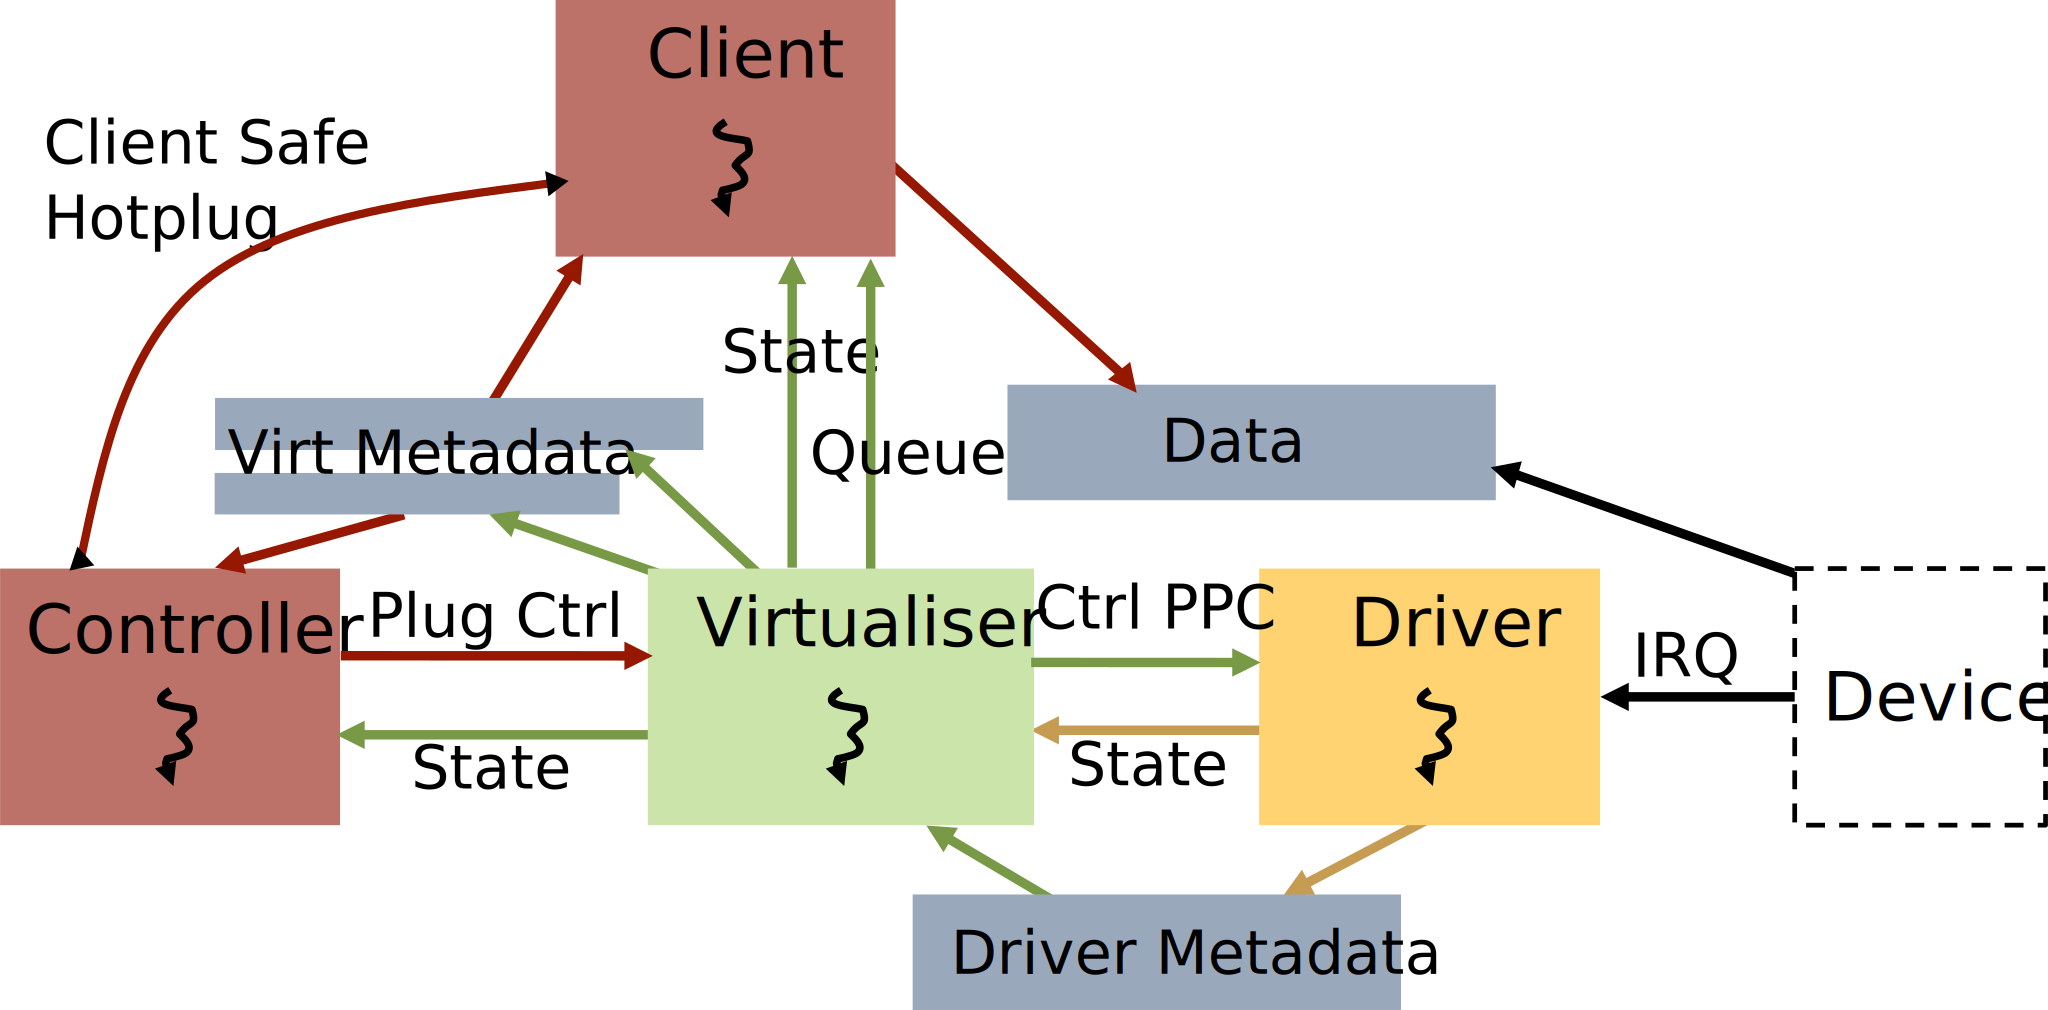
\includegraphics[scale=\figscale]{hotplug_safe_eject}
  \caption{A structure showing how a controller can request device ejection.}
  \label{f:hotplug_safe_eject}
\end{figure}

We assume that we have a specific privileged client that we designate as
the \emph{controller client} that acts as the human interface to the system.
We broadly have two approaches that we could take:

\begin{enumerate}
\item The controller client talks to the virtualiser, which notifies all of
      the downstream clients (who have to notify any further downstream
      clients, in the case of a filesystem client for a block virtualiser).
      The clients can then safely stop, and notify back up the chain to the
      virtualiser, who can then request the driver to eject.

\item The controller client talks directly to all the leaf clients to safely
      stop, and these clients respond when complete.
\end{enumerate}

The advantage of (1) is that we re-use the existing virtualiser
infrastructure, and so do not need to map extra pages into the clients.
However, we cannot effectively re-use the existing virtualiser. We would
have to re-use the \emph{Block State Notification} to notify clients,
who then, in the case of a filesystem, need to notify their clients is
some other way. Also, this approach will not work for  device classes.

In contrast, (2) imposes the exact same burden on clients -- being
notified and responding - but does not require modifications to the
virtualiser and intermediary clients. In addition, policies regarding
timeouts waiting for ``ready for ejection'' events are implemented within the
controller client, not the virtualiser, which is simpler. The only
distinction between a safe ejection and an unsafe one is in the
clients, from the virtualiser and driver's perspective it is just an
ejection.

We implement option (2) with a thin wrapper over notifications in
\texttt{include/sddf/hotplug/clients.h}. A shared page for each client
is mapped R/W in the controller, and R/O in each client, containing a
boolean representing the pending eject state. The controller can call
\texttt{hotplug\_set\_pending\_eject()} to notify the clients of an
ejection request, who respond with a ppcall back in
\texttt{hotplug\_ready\_for\_eject()}. In our sample implementation, the
controller waits for all clients to respond, but this policy could
easily be changed.

\section{Limitations}

\begin{enumerate}
  \item There are race conditions with block queues during a quick eject and insert request.
        Requests sent for the old device could end up being sent for the new one,
        from the perspective of the virtualiser and driver.
        Each block request needs to be tagged with the device ID or a generation
        number so old requests can be invalidated.

  \item Initialisation failures are not communicated to the clients.
\end{enumerate}


\chapter{Device Discovery}\label{s:discovery}

There is \textbf{preliminary} work on extracting device parameters
from the Linux \emph{device tree} specification as part of
configuration tool for the seL4 Microkit~\citep{microkit:url}.
This is not yet in a halfway stable state. We will
describe this in a later version. \DEFER{Device-tree extraction.}

Currently, it is expected that the system designer knows all the
devices that will be available and used, and can choose components and
assign memory manually to use all the devices that are needed for the
system being built.

\chapter{Leveraging Linux}\label{s:linux}

Note: This chapter is \textbf{preliminary}.

\section{Component development}

The Linux \emph{userspace I/O} (\gls{uio})
mechanism~\citep{linux:uio}, designed to support usermode drivers,
allows mapping physical memory regions uncached into Linux user space.

We can use this to develop \gls{sddf} virtualisers and device drivers in
Linux user space, on a Linux system running inside a \emph{virtual
  machine} (\gls{vm}) on top of seL4. This allows us to use the normal Linux
development tools for component development. While not suitable for
performance analysis and tuning, this can simplify and accelerate
development.


\begin{lstlisting}[gobble=2,firstline=2,float=th,tabsize=2,
  label={l:uio_config},
  caption={Example \gls{uio} stub driver command-line configurations.}]

  chosen {
     bootargs = "... uio_pdrv_genirq.of_id=sddf_framebuffer ...";
  };
\end{lstlisting}

\gls{uio} works with a stub driver in the Linux kernel.  There are two
generic drivers provided in the mainline Linux source tree,
\code{uio\_pdrv\_genirq} and \code{uio\_dmem\_genirq}.
\code{uio\_pdrv\_genirq} is used when the device is not a
bus-mastering \gls{dma} controller; \code{uio\_dmem\_genirq} when the device
can do \gls{dma}.  These drivers do not specify which devices they are
compatible with; they can be bound to a particular device in various
ways.  We usually bind at boot-time using a Linux kernel command line
argument as shown in \autoref{l:uio_config}.

\begin{lstlisting}[gobble=2,firstline=2,float=th,tabsize=2,
  label={l:uio_node},
  caption={Example \gls{uio} node in device tree.}]

  uio@0x30000000 {
     compatible = "sddf_framebuffer","uio";
     reg = <0x00 0x30000000 0x00 0x2000000>;
     interrupts = <GIC_SPI 18 IRQ_TYPE_EDGE_RISING>;
  };
\end{lstlisting}

To use \gls{uio}, a node describing the interface is added to the device
tree handed to the virtual machine.  For details, see the device-tree
specifications in the Linux source tree, \autoref{l:uio_node} shows an
example.

You can choose the \code{compatible} string to be whatever does not
clash with a real device.
\iffalse
\gernot{What's the ``compatible string'', hasn't been
  mentioned before. \code{login} doesn't have a man entry for either
  of the above functions.}\peterc{They're device drivers in the Linux
  kernel, not functions.  Each device tree node has a string, labelled
  'compatible' that says what kind of device it is.  Each device
  driver in Linux provides a list of strings for the devices it can
  drive.  The full list of strings->drivers is available to Linux at
  boot time; it goes through the device tree and tries the probe
  function for each driver (loading modules if necessary)
  where the compatible strings match.  (This is necessary because some
  devices have the same identification even though they are different,
  and need different drivers.  There are ethernet devices where there
  are about four different versions all with the same model number).
  The first such probe routine that returns a success is used; failed
  drivers are unloaded from the kernel.  Is this the place for a
  detailed discussion of what a device tree is and how Linux uses it for
  driver binding?  The generic drivers above do not pre-specify
  compatible strings; you can either bind them at boot time on the
  Linux command line, or at run time by loading the module with module
  arguments, or, if it is already loaded, creating and binding a new
  instance by manipulating the files in /sys/modules/<drivername>}
\fi
The \code{reg} parameter needs to give the addresses of the
regions. When running \gls{sddf} (and the development \gls{vm}) on top of the seL4
Microkit~\citep{microkit:url}, this will need to match the address of
the memory region specified in the Microkit's \emph{system description file}
(SDF), to ensure that
Linux and the \gls{sddf} component under development see these regions at
the same address.

The above example specifies a single
32\,MiB region at (virtual-machine) physical address 0x30000000.
Likewise, the \code{IRQ} parameter gives the \gls{irq} controller, \gls{irq}
number (relative to the first interrupt on that controller) and the
type.  Again this must be different from any other interrupt in the
device tree.

The virtual-machine monitor (\gls{vmm}) maps each interrupt onto a separate Microkit
\emph{channel}. If such a channel is connected to the \gls{vm}, a
notification on that channel (resulting from an interrupt or a
notification from another component) will result in injecting the
corresponding virtual interrupt into the \gls{vm}. When the \gls{vm} re-enables
that (virtual) interrupt, this triggers a notification to the Microkit
protection domain at the other end of the channel, or an interrupt
acknowledgement operation (if the notification was from a real
interrupt).

A usermode program running in the \gls{vm} can then use \code{mmap()} calls
on
\code{/sys/class/uio}\(N\)\code{/maps/map}\(n\)\code{/addr}
to access metadata and data regions,
\code{read()} or \code{poll()} system calls  on
\code{/dev/uio}\(N\) to wait for notifications,
and \code{write()} on the \gls{uio} device file to generate
notifications. Here, \(N\) identifies the \gls{uio} device (of which there
can be several), while \(n\) refers to the \gls{uio}-mapped region of the
device (of which there can be multiple as well).

Most of this is abstracted into a (still under development) \code{libuio} library, making it
possible to write components that are relatively easy to port between
Linux user space and native Microkit. \DEFER{Add to Lions OS.}
\iffalse
\gernot{Is this library part of
  the \gls{sddf} release? Or rather of Lions OS?}\peterc{It's in LionsOS;
  hasn't been merged yet.  Used by the Block Device driver \gls{vm}.  The
  framebuffer driver \gls{vm} doesn't use it yet.  FB needs to be
  merged before release.}
\fi

In addition, one can prevent the Linux in-kernel driver from binding
to a particular device, by changing its \code{compatible} string in
the device tree.  One can then bind it to a \gls{uio} stub driver and write
a user-mode \gls{sddf}-style driver that runs in Linux userspace on the guest.

\begin{figure}[ht]
  \centering
  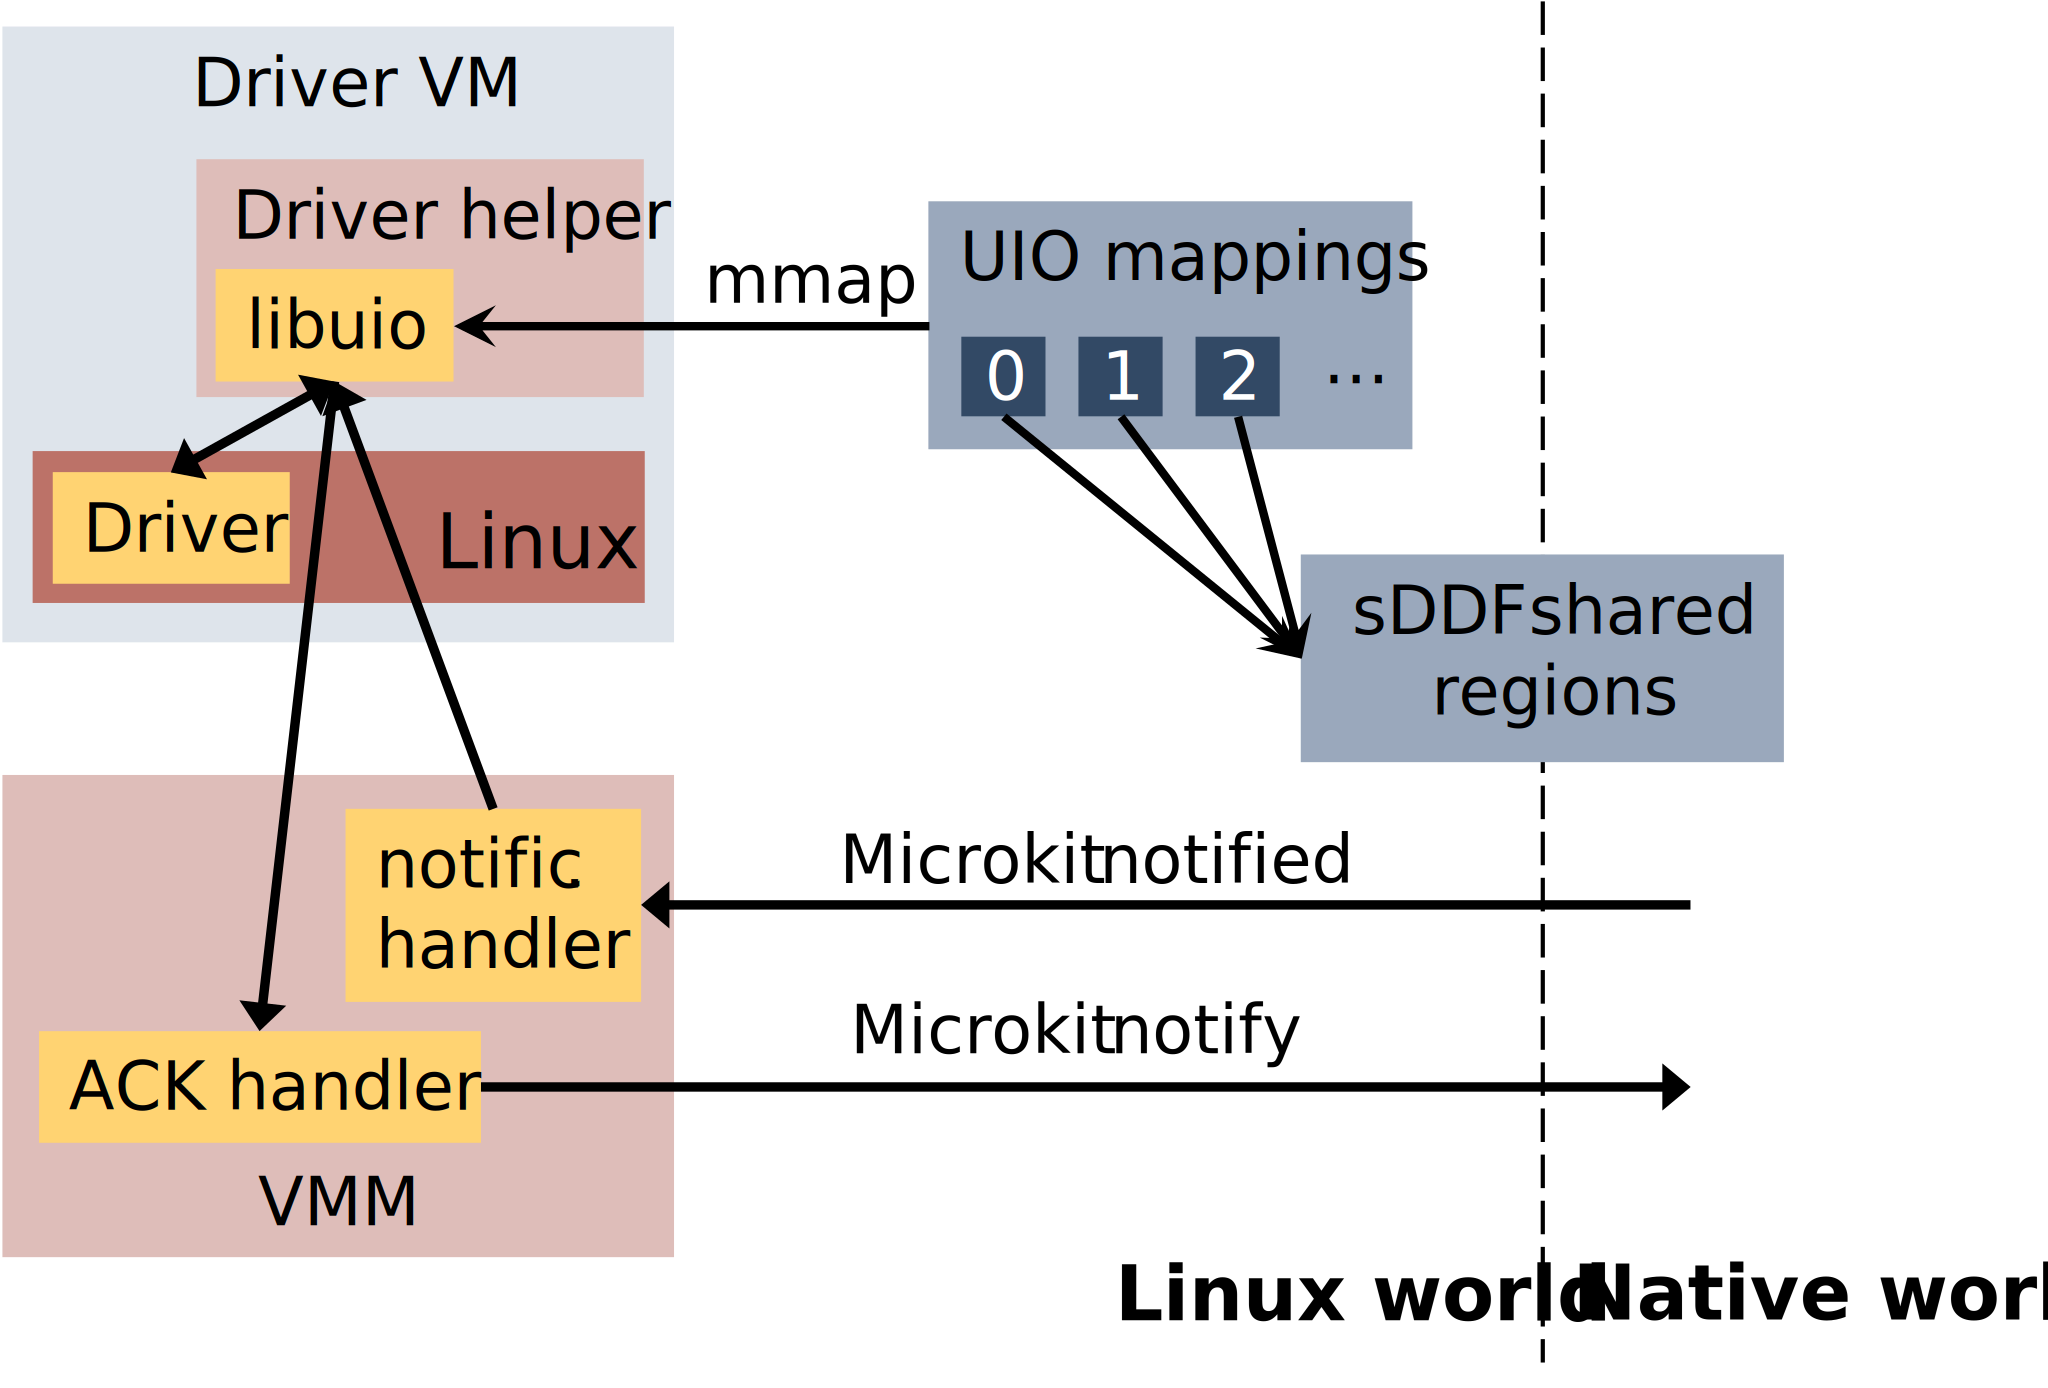
\includegraphics[scale=\figscale]{uio-drivers}
  \caption{Linux driver re-use through \gls{uio}.}
  \label{f:uio-drivers}
\end{figure}

\section{Legacy driver reuse}

Instead of developing drivers in Linux, we can use the same setup for
re-using existing Linux drivers in the \gls{sddf}. A virtualiser connects to
a ``driver PD'' that is in reality a Linux \gls{vm} containing the
driver and a userspace program, the \emph{driver helper}, that
interacts with the \gls{sddf} using the above \gls{uio} mechanisms, as indicated
in \autoref{f:uio-drivers}.

\begin{lstlisting}[gobble=2,firstline=2,float=th,tabsize=2,
  label={l:linux-block},
  caption={[Example of Linux usermode driver helper.]Example of a
Linux usermode driver helper for a block device accessed via a regular Linux file (simplified).}]

  notified(int channel) {
    needs_notify = false;
    while (dequeue_request(request_queue, &request)) {
      switch (request.storage_command) {
        case READ_BLOCKS:
          llseek(fd, BLOCKSIZE*request.block_number, SEEK_SET)
          count = read(fd, adjust_address(request.address),
                          BLOCKSIZE*request.block_count);
          response.count = request.block_count;
          response.success = count/BLOCK_SIZE;
          response.result = count == BLOCKSIZE * request.block_count
                            ? SUCCESS : map_error(errno);
          enqueue_response(response_queue, &response)
          needs_notify = true;
          break;
          ...
      }
    }
    if (needs_notify)
      notify(channel);
  }
\end{lstlisting}

The driver helper forwards \gls{sddf} requests to the Linux in-kernel
driver using standard Linux \gls{io} mechanisms. This can be as simple
as reading block-sized chunks from a Linux block
device, or even a regular file, using normal Linux
\code{read} or \code{write} calls, as shown in
\autoref{l:linux-block}. The \code{notified()} function is invoked by
\code{libuio} when the notification channel is signalled. The
\code{notify()} function writes to the appropriate \code{/dev/uio}
special file to cause a notification by the \gls{vmm} on the corresponding
channel.

The virtualiser code is unaware of whether the driver is
native or a driver \gls{vm}, the only difference is that the driver metadata
region must be configured as \emph{uncached} in the Microkit SDF.

Obviously this approach will not result in high-performance drivers,
nor can Linux drivers be trusted, but most drivers are not
particularly performance-sensitive, and trust can be minimised by
encrypting data that is sent to the device (reducing the potential
attacks to denial of service). These limitations are frequently
acceptable, particularly if this allows obtaining complex drivers for
free.

In such a case, the Linux instance should be reduced to the bare
minimum to support the driver in question, as
demonstrated many years ago by \citet{LeVasseur_USG_04}.

\chapter{Security Analysis}\label{s:security}

Note: This chapter is \textbf{preliminary}.

An implication of the threat model of \autoref{s:threats} is that any
trusted component of the system must be verifiable. Another implication is
that components that interface with untrusted components must sanitise
their inputs.

The design of our queues means that
pointers into those queues are automatically sanitised (the index is
taken modulo the queue size). Similarly, pointers into the data and metadata
regions on the client-side of the virtualiser are all offsets into the
respective region and only need a check that they do not exceed the
region size. These requirements should be easy to verify.

\section{Trusted components}

For now we assume all the components of the \gls{sddf} to be trusted, specifically:
\begin{itemize}
\item drivers are trusted
\item virtualisers are trusted
\item copiers are trusted.
\end{itemize}
In addition, the device hardware is (currently) trusted.

Untrusted device drivers or devices should be achievable, provided that:
\begin{itemize}
\item all data handled by the device is encrypted and signed (using
  higher-level protocols);
\item denial of service by the device or driver is not considered a
  threat;
\item the device is not \gls{dma}-capable, or its access is restricted by
  suitable \gls{iommu} mappings (managed by the virtualiser);
\item the virtualiser sanitises all references received from the client.
\end{itemize}
\DEFER{Check proper sanitation of driver VMs!}

\section{Verifying components}

The driver model is designed to simplify drivers dramatically
(compared with e.g. Linux drivers).  Drivers are simple state machines
free from internal concurrency (but do access/modify data structures
that are concurrently accessed/modified by hardware). In fact,
experience with Ethernet drivers shows that they are so simple that
little debugging effort is required to achieve correct
functionality~\citep{Parker:bsc}.

The simplicity should make it finally feasible to formally verify
drivers for non-trivial real-world devices, such as \glspl{nic},
although verification requires not only formalising the driver framework
but also the device interfaces.

Similar arguments apply to virtualisers: they are also kept
simple (even simpler than drivers)  and
should be verifiable.

The use of virtualisers allows simplifying the IP stack as well, as it
only handles packets for a single client and does not have to deal
with broadcast requests. Such a simple IP stack may be verifiable as
well, and there is work attempting exactly this~\citep{Rollins_23}. A
verified IP stack may eliminate the need for copiers.

When blocking on a response (Notification or IPC reply) from an
untrusted component, a trusted component may have to employ a watchdog timer
to prevent indefinite blocking, depending on its purpose.

\section{Verifying component interactions}

Simplifying drivers and virtualisers by removing any internal
concurrency potentially shifts some of the complexity into the driver
framework itself, including concurrency. In fact, our experience shows
that the dominating debugging task is not of the driver/virtualiser
functionality, but the inter-component signalling protocol. Achieving
deadlock freedom is not difficult in itself, but achieving it without having
components perform unnecessary signals resulting in other components
being awoken without having useful work to perform is the challenge.
Optimisations to the simplest policy of "signal each time work has been
done" can easily lead to unforeseen deadlocks or delays in processing
further down the line, and without the use of an automated tool it can
be difficult to calculate by hand whether potential optimisations could
lead to a stagnation in the system.

Thus, this is an ideal use case for model checking, and we have developed
simplified abstract models of our networking components in order to verify
that each optimisation to our signalling protocol cannot lead our system into
deadlock. As the signalling protocol is updated during development, we are
able to update our abstract models accordingly and rerun them through the
verification tool to ensure that we have not inadvertently introduced any
issues.

An advantage of the \gls{sddf} model is that this complexity is encapsulated in a
relatively small code base, and the verification needs to be done only
once per device class (and not for each individual driver).

The sanitation requirements on drivers and virtualisers apply to the
framework implementation as well, and should be verified.

\chapter{Implementation Status}\label{s:status}

The \gls{sddf} is implemented as described above on top of the seL4
Microkit~\citep{microkit:url}. The Microkit simplifies the
implementation (among others) by moving the handler loop (see
\autoref{f:eth_driver}) into the framework, so the driver and
virtualiser implementations mostly consist of the notification handler
functions.

The Microkit implementation presently provides high-performance
networking (see \autoref{s:performance}). There are a implementations for a number of other device
classes (serial, \gls{i2c}, storage, graphics, audio) which are still in a
preliminary state. The framework is presently based on active
virtualiser and driver components.

The code accessible on GitHub under a BSD license:
\url{https://github.com/au-ts/\gls{sddf}}.

\chapter{Performance}\label{s:performance}

\section{Performance evaluation setup}

\begin{figure}[th]
  \centering
  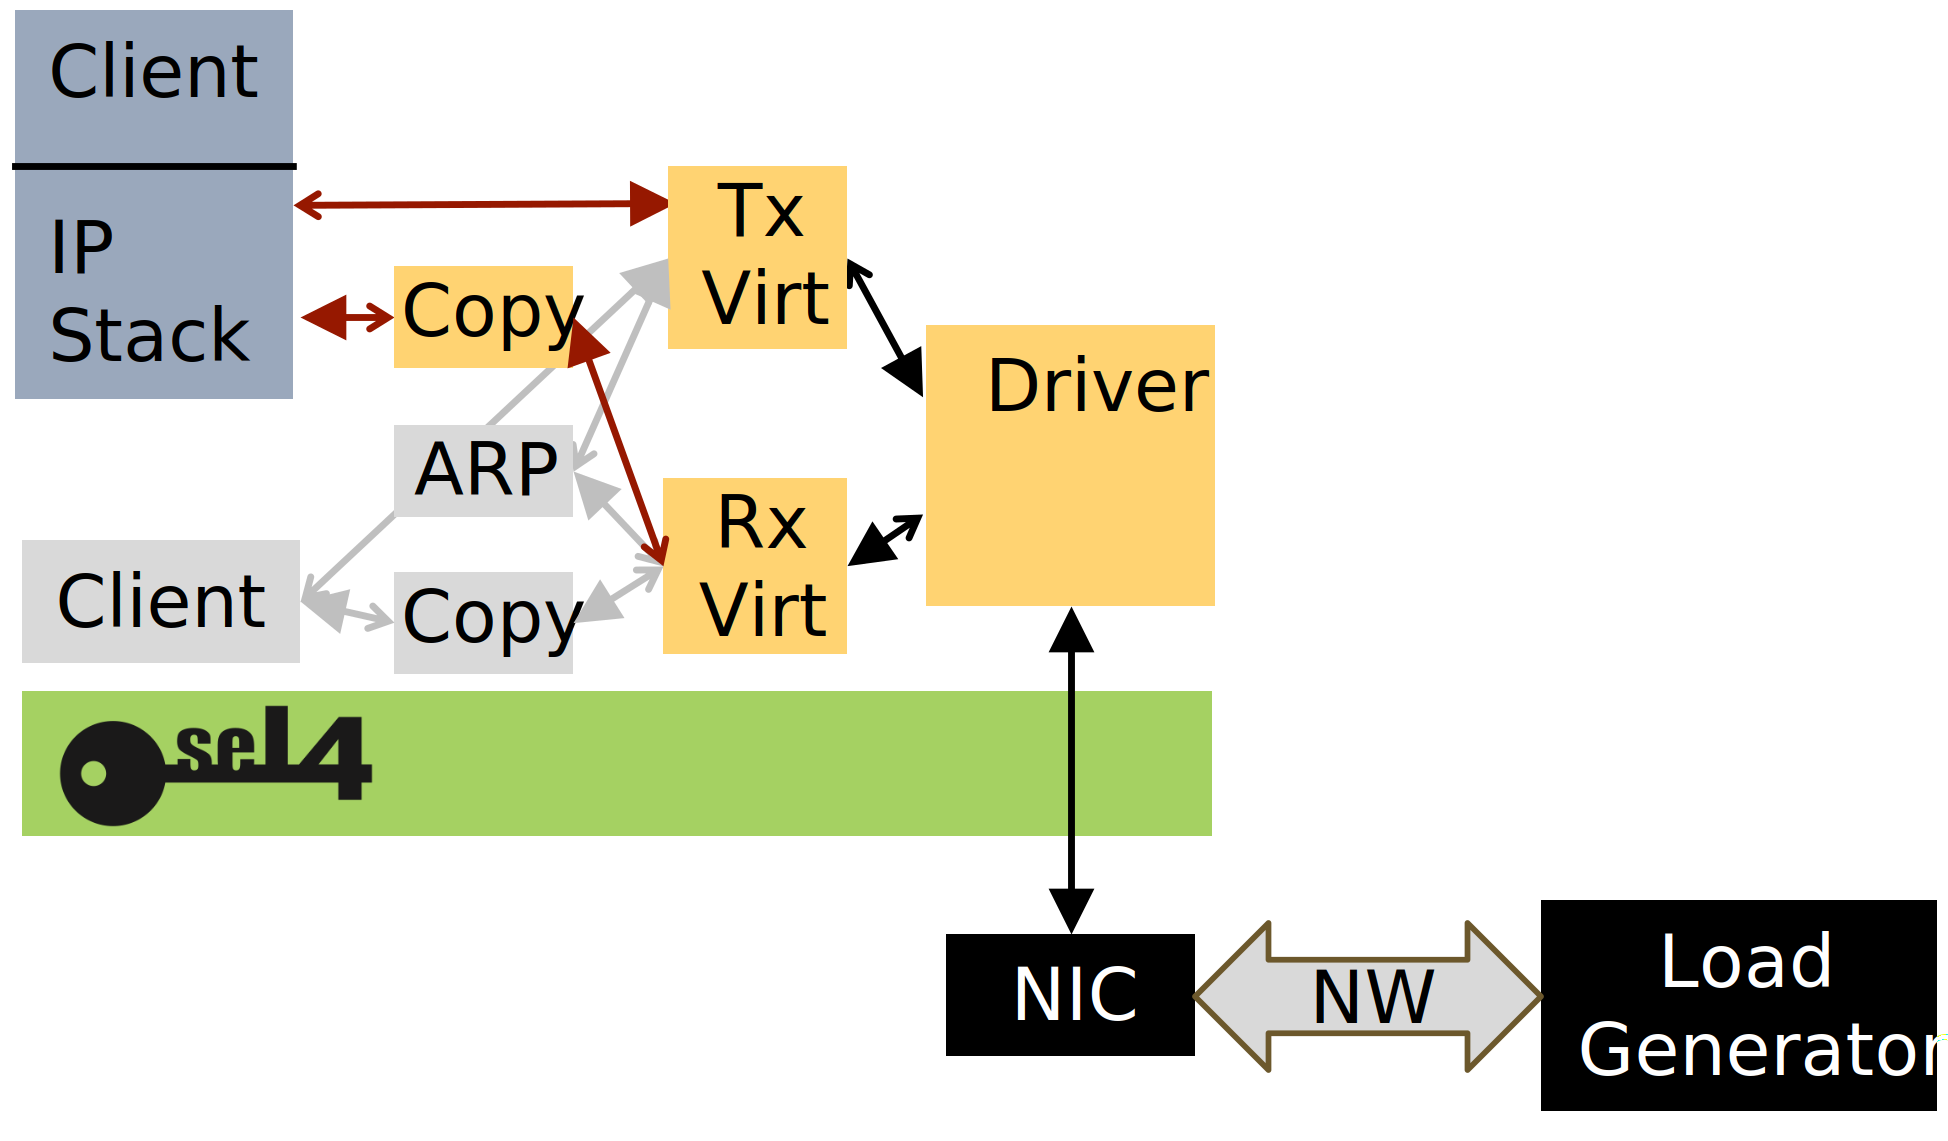
\includegraphics[scale=\figscale]{setup-sddf}
  \vspace{5ex}
  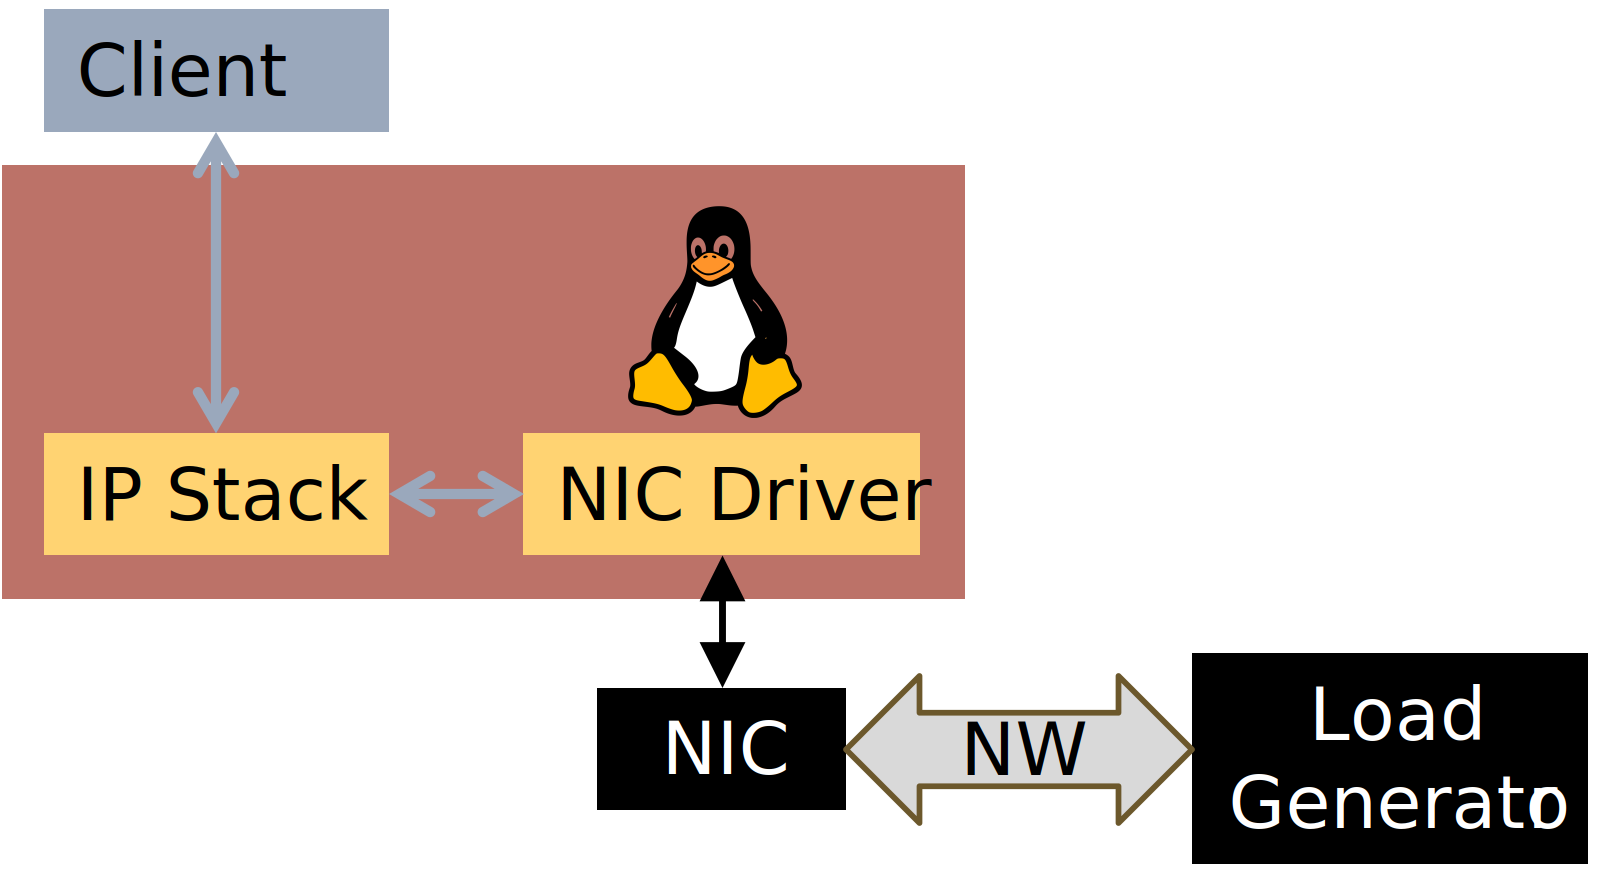
\includegraphics[scale=\figscale]{setup-linux}
  \caption{Evaluation setup for \gls{sddf} (top) and Linux (bottom).}
  \label{f:setup}
\end{figure}

We evaluate \gls{sddf} networking performance against the older CAmkES-based driver
framework, as well as against Linux.

The evaluation platform is an Arm Cortex-A53 processor based on the
i.MX8M Mini microarchitecture running at 1.8GHz, equipped with a
Gigabit Ethernet \gls{nic} using a 10/100/1000 Atheros AR8031 \gls{phy}. We run
\emph{ipbench}~\citep{Wienand_Macpherson_04} for distributed load
generation from four client machines, each sending UDP packets to the
seL4-based target machine, which sends them through an IP stack
(\emph{lwIP}~\citep{Dunkels_01}) to a co-located client, which
returns the packets, slightly modified according to the ipbench protocol.
The load generators count the successful
replies to determine the achieved throughput and latency, while a
low-priority thread on the target machine measures idle time to
determine the \gls{cpu} load imposed by the test.

\autoref{f:setup} shows the setup.
The \gls{sddf} system is based on the seL4 Microkit~\citep{microkit:url}.
Linux benchmarks use a Linux 6.1.1 kernel system on the same hardware.

\section{Performance results}
\FIXME{Update to the data from the SOSP submission, which is much better!}

\iffalse
\begin{Comment}{For internal reference:}
  Performance data sources:
  \begin{itemize}
  \item Lucy's original data:
    \url{https://docs.google.com/spreadsheets/d/1neMwJeKgMkRQvPDG8GXoqAUji8KJyAp9RC0tyuH-wEo/edit#gid=1264566754}
  \item Lucy's thesis repo: \url{https://docs.google.com/spreadsheets/d/1neMwJeKgMkRQvPDG8GXoqAUji8KJyAp9RC0tyuH-wEo/}
  \item Courtney's data: \url{https://docs.google.com/spreadsheets/d/1d1hKhZVVbEvxm7ehs7sXc1KvGjfdJ0RHR4YiMPzR8O8/edit#gid=1272856437}
  \end{itemize}
\end{Comment}
\fi

\subsection{Simplified system, CAmkES, Linux}\label{s:p-camkes}

We initially evaluate a simplified two-component system, where the
client, IP stack and cache management are merged into a single component (no device
sharing supported), and only the
driver is separate. This setup, while not very realistic, is directly
comparable to the older driver framework based on
\gls{camkes}~\citep{Kuz_LGH_07}. We also convert the
\gls{camkes} framework to our transport layer and run it in the same,
two-component configuration.

\begin{figure}[th]
  \centering
  \includegraphics[width=\textwidth]{s-camkes-linux}
  \caption[\gls{sddf} networking performance compared to other systems
  running single-core.]{\gls{sddf} networking performance, compared to original CAmkES,
    CAmkES with the new transport layer, and Linux. All benchmarks use
    a single core.}
  \label{f:s-camkes-linux}
\end{figure}

% Initial benchmarks we made prior to implementing the lightweight asynchronous transport layer between the 2 components shows poor performance.
\autoref{f:s-camkes-linux} shows the results. We can see that the
original \gls{camkes} system already reaches 66\% \gls{cpu} utilisation at
200\,Mb/s applied load, and can be expected to saturate the \gls{cpu} at
around 350\,Mb/s.\footnote{The measurements on ``original CAmkES''
  (in fact after a fair amount of performance tuning) were done in 2021
  and we only have records for the low-load cases.}

\gls{camkes} adapted to the new transport layer  (``new CAmkES'') uses somewhat less \gls{cpu} (52\%
vs. 66\% at 200Mb/s, a 20\% improvement) but maxes out the \gls{cpu} above a load of
400\,Mb/s. Achieved throughput  scales with applied load to 600\,Mb/s, and then collapses
when applied load exceeds 700\,Mb/s. Performance
collapse under overload is not untypical in network systems, and
generally results from latency blowout.

Linux behaves somewhat better, also scaling just over 600\,Mb/s, when it saturates
the \gls{cpu}. While nowhere near as extreme as the performance collapse of
\gls{camkes}, Linux throughput still degrades somewhat under overload.

In contrast, the \gls{sddf} system scales linearly to the wire
speed.\footnote{Note that a Gigabit Ethernet \gls{nic} can handle about
  950\,Mb/s of payload with standard 1.5\,KiB Ethernet frames, the rest of the bandwidth is lost to
  Ethernet headers and inter-packet gaps.} It
does \emph{not} max out the \gls{cpu}, but handles the full applied load
with only 60\% \gls{cpu} utilisation, leaving plenty of performance
head space. At all load levels it uses far less \gls{cpu}
than Linux. At low load (100\,Mb/s), the \gls{sddf} \gls{cpu}
usage is 12\%, beating all the other systems by a factor of 1.9 or
more. The ratio becomes smaller at higher
load due to batching.

\subsection{Cost of modularity and security}\label{s:modul}

\begin{figure}[t]
  \centering
  \includegraphics[width=\textwidth]{s2-s5-linux}
  \caption[Performance of differently modularised \gls{sddf} systems compared to Linux.]{Performance of a two-, four-, pseudo-five- and  a standard
    five-PD \gls{sddf} system compared to Linux, all on a single core.}
  \label{f:2-5-PD}
\end{figure}

Now we compare the simplified two-PD system to the more realistic one
of \autoref{f:setup}, where five PDs (out of a total of 8) are involved in handling each
packet, \emph{and} incoming data is copied to separate client address
spaces. For more analysis, we present also two intermediate systems: a
four-PD system, which has the Copier component removed, and a
pseudo-five-PD system (labelled ``p5-PD'') where instead of a copier
we have a dummy component that just forwards packets without doing any
meaningful processing.

\autoref{f:2-5-PD} shows the results.
We can see that the three extra context switches plus one data copy
increase \gls{cpu} usage noticeably, from 12\% to 19\% at 100\,Mb/s,
and from 60\% to 77\% at high load, a relative increase of 64\%
at low load and 27\% at high load (again, the effects of overheads are
lessened by batching).
Yet, this highly modular setup still clearly outperforms Linux by
more than a factor 1.5 (low load).

\begin{figure}[t]
  \centering
  \includegraphics[width=\textwidth]{s2-s5-linux-cyc}
  \caption{Comparing per-packet processing costs of the four \gls{sddf} systems.}
  \label{f:2-5-PD-cyc}
\end{figure}

The intermediate systems show that the extra data copy plays a similar
role as the extra context switches, and they all add low to moderate
overheads. This becomes clearer in \autoref{f:2-5-PD-cyc}, which
compares per-packet processing costs. It clearly shows that the
difference between the 4-, pseudo-5- and 5-PD systems is fairly
small: the extra PD (without copying) increases per-packet processing cost by
1.5k cycles at 100\,Mb/s and 350 cycles
at wire speed, a relative increase of 8\% and 4\% respectively. In
comparison, copying adds 700 cycles at low and 1,000 cycles at high
load, a relative increase of 3\% and 11\% respectively.\footnote{One
  would expect the absolute per-packet copying cost to be independent of
  load. We did not investigate this further, but suspect caching effects.}

\subsection{Multicore}

\begin{figure}[t]
  \centering
  \includegraphics[width=\textwidth]{kernel-sc-mc}
  \caption[Single-core \gls{sddf} performance with single- and multicore
  configurations.]{Single-core \gls{sddf} performance using single core seL4
    kernel with and without memory barriers enabled vs multicore
  seL4 kernels.}
  \label{f:kernel-sc-mc}
\end{figure}

All the above benchmarks were run on a single core, using an system
that is optimised for that case: the seL4 kernel compiled with
multicore support disabled, and no memory barriers in the \gls{sddf}
queue libraries.

Enabling multicore increases
the baseline system-call cost of seL4 by about 50\%, basically the
cost of acquiring and releasing the kernel lock. Additionally,
supporting a multicore system requires memory barriers when enqueuing
or dequeuing entries in the shared queues, to ensure they work
correctly of the other PD accessing the queue runs on a separate core.

The \gls{cpu} load figures in \autoref{f:kernel-sc-mc} show that both
requirements add similar overheads. Here we compare the strict
single-core configuration used so far (``SC kernel'') with a version
that adds the memory barriers but still uses the single-core kernel
(``MB-SC kernel''), and additionally the same \gls{sddf} version running on
seL4 with multicore enabled (``MC kernel''). Adding memory barriers
adds about 15\% overheads at low load and 8\% at high load, while the
total cost of enabling multicore is almost 50\% at low load and almost
20\% at high load.

\begin{figure}[t]
  \centering
  \includegraphics[width=\textwidth]{sc-mc-linux}
  \caption[Single- and two-core \gls{sddf} performance compared to 2-core
  Linux.]{Performance of \gls{sddf} running single-core (\gls{sddf}~SC) vs.\ distributed over
    two cores (\gls{sddf}~MC) compared to Linux running on two (Linux~2C) or
    four (Linux~4C) cores.}
  \label{f:sc-mv-linux2}
\end{figure}

From now on we use the kernel and \gls{sddf} version that fully supports multicore.
We compare multicore-enabled \gls{sddf} running on a single core
with \gls{sddf} with its components distributed over two cores:
the driver and \gls{tx} virtualiser run on one core,
and the other components, Client, Copier and \gls{rx} virtualiser, on the other. We
compare to two Linux configurations, one restricted to two cores and
the other giving it free choice of all four cores.c

The results are in \autoref{f:sc-mv-linux2}.
Having 2 cores at its disposal, Linux just manages to handle the
applied load (as indicated by latencies, which increase significantly
at the highest applied load). Its \gls{cpu} usage is well above that of the
\gls{sddf} system. On four cores, Linux shows significantly higher overall
\gls{cpu} load, while still barely coping with the network load (indicated
by the \gls{cpu} usage blowing out at 950\,Mb/s, and also reflected in a
latency blowout).

In contrast, the \gls{sddf} system still has significantly lower \gls{cpu}
utilisation than Linux, total \gls{cpu} load staying (just) below 100\% of
one core even at the highest network load. The total \gls{cpu} load of the
two-core configuration is 65\% higher (31\% vs 19\%) than the
single-core version at low load and 30\% higher (98\% vs 77\%) at high
load. This is due to
cross-core notifications being more expensive than intra-core
notifications.

The overall \gls{cpu} load of an \gls{sddf} system will obviously be sensitive to
the allocation of PDs to cores, which, in turn, depends on other
considerations, such as maximising cache locality or freeing up cores
for other activities. The optimal configuration will therefore be
dependent on the use case. The multicore-enabled configuration
provides full location transparency to PDs.

\section{Discussion}\label{s:perf-disc}

The framework, running on the Microkit, clearly over-achieves our goal
of ``performance comparable to Linux'', outperforming Linux by a
significant margin under all configurations evaluated. Performance is vastly better than that
of the \gls{camkes} system adapted to our transport layer (which is already
a significant improvement over the performance of the previous \gls{camkes}-based
driver framework).

The performance comparison to Linux is especially encouraging, given
that the Linux IP stack is supposedly well optimised (especially for
multicore use), while we are using the simple
lwIP~\citep{Dunkels_01}. We find that even on multicore (the scenario
most favourable to Linux) our per-packet costs are significantly lower.

Parker~\citep{Parker:bsc} conducted a more comprehensive performance
analysis, including highly asymmetric (send-mostly or receive-mostly)
traffic, multiple active clients with traffic shaping, more multicore
configurations, and forcing the system to be overloaded.
The evaluation confirmed that the \gls{sddf}/Microkit system shows no
performance collapse under any overload conditions evaluated, unlike what we observed in
\autoref{s:p-camkes} for the \gls{camkes} system.

The evaluation, specifically the results shown in \autoref{s:modul},
provide strong justification for our highly modular design: The cost
of a PD switch is small compared to the base processing cost.

This confirms the original hypothesis driving
the \gls{sddf} design: Context-switching costs (of the order of 400--500 cycles
for the single-core kernel on our Armv8 platform, about 50\% higher
for the multicore kernel, and still higher for cross-core
notifications) are not a major factor. In fact, we measure
handling costs of less than 50,000~cycles per packet on \gls{sddf} under any
conditions, and no more than about 12,000~ cycles under high network
load. Hence, the pure kernel overhead of adding an extra component
(two system calls) to
the packet-processing pipeline adds no more than about 15\% (usually
much less) to the handling cost.

As such, our main take-away is that the fine-grained modularisation,
resulting from the strict separation of concerns, works and adds
far less overhead than the complexity of the Linux system. The reason is two-fold:
\begin{enumerate}
\item as stated, context-switching costs in seL4 and the Microkit are
  small enough to not significantly impact performance, and
\item the \gls{sddf} model encourages implementation simplicity that can
  \emph{reduce} overheads (which is the reason \gls{sddf} outperforms Linux).
\end{enumerate}

The latter has further, highly encouraging implications: We can keep
individual component implementations very simple, without sacrificing
performance. This simplicity not only greatly reduces debugging
efforts, it should also make automatic verification techniques
applicable. The experience with verifying the
Microkit~\citep{Paturel_SH_23} gives us confidence that this should be
achievable.

The evaluation of the multicore configurations are also highly encouraging: It shows that the \gls{sddf}
naturally distributes across cores. While all PDs are strictly
sequential (resulting in decreased code complexity), the design makes
them location-transparent, meaning they can be arbitrarily allocated to cores
in order to balance load. The evaluation confirms the feasibility of
this design choice of keeping components sequential and instead allowing arbitrary concurrency
\emph{between} components.

Further performance improvements seem possible with improvements to
the kernel itself. Candidates are fast-pathing notifications to
higher-priority threads, and taking notifications out of the kernel lock.


\chapter{Conclusions}

We have developed a low-overhead device driver
framework for seL4, \gls{sddf}, implemented it on the seL4 Microkit, and
comprehensively evaluated it on network devices. It is based
on a highly efficient, asynchronous zero-copy transport layer using
lock-free single-producer, single-consumer, bounded queues.

Measured performance shows a vast improvement over the
\gls{camkes}-based framework, as well as significantly better performance than
Linux, despite the higher number of system calls and context-switches
required. In particular we find that a highly componentised \gls{sddf}
system easily distributes across cores, while each individual
component being strictly sequential, reducing its complexity.

So far we have only examined the performance of the network system. We
have started applying the same ideas to other device classes,
especially storage. Other device classes are generally much less
sensitive to system performance than networking, so we do net expect
any surprises there.

We are also working on integrating \gls{sddf} with the Microkit's
virtualisation infrastructure, which will support \glspl{vm} as clients as
well as drivers and virtualisers. On the one hand, this provides a
convenient way of developing \gls{sddf} components as Linux programs that
can later be converted into native \gls{sddf} PDs. On the other hand, this
allows re-use of existing Linux drivers in the form of a driver-\gls{vm}.

Obviously, such legacy drivers are in no way trustworthy. Furthermore,
virtualisation overheads are expected to dominate
\gls{sddf} overheads, so these configurations are important for
functionality (especially the ability to re-use unmodified Linux
drivers) but will not be suitable for performance-sensitive
devices.

%\clearpage
\bibliographystyle{plainnat}
%\addcontentsline{toc}{chapter}{Bibliography}
\bibliography{references}

\appendix

\chapter{OS Abstraction}\label{s:osal}

The \gls{sddf} is meant to be usable by all seL4-based \glspl{os}. As
such it needs an abstraction layer for invoking underlying \gls{os}
services. This abstraction layer consists of a number of (inlineable)
functions that map the mechanisms required by the \gls{sddf} to the
underlying \gls{os}.

\section{Microkit Mapping}\label{s:mkal}

The seL4 Microkit provides a small number of abstractions:
\begin{itemize}
\item a \emph{\gls{pd}} is an address space plus a thread of control.  It has
  a name, and a priority for its thread; in addition its budget can be
  controlled,
\item a \emph{channel} is a small integer that is passed with a
  notification, to identify what kind of notification it is
\item a \emph{notification} is an asynchronous signal between PDs
\item a \emph{\gls{ppc}} is a synchronous signal, that can pass values
  in a number of \emph{message registers}.
\end{itemize}

The sDDF mechanisms map one-to-one onto these abstractions.

A PD has up to three entry points.  Its \texttt{init()} entry point is
called when the PD first runs; after \texttt{init()} returns, the
\texttt{notified(channel)} entry point is invoked whenever the PD
receives a notification from another PD or from an interrupt source.
The \texttt{protected(channel)} entry point is invoked from a
\gls{ppc} call from another PD.

\begin{lstlisting}[firstline=2,float=th,tabsize=2,
  label={l:sddf-interface},
  caption={sDDF interface functions.}]

/* Return the name of the currently running protection domain */
char *sddf_get_pd_name();

/* Acknowledge an interrupt */
void sddf_irq_ack(sddf_channel ch);

/* Notify a channel */
void sddf_notify(sddf_channel ch);

/* Generate a notification, but not until this PD is about to sleep */
void sddf_deferred_notify(sddf_channel ch);

/* Acknowledge an interrupt, but not until this PD is about to sleep */
void sddf_deferred_irq_ack(sddf_channel ch);

/* Return any outstanding deferred notification */
unsigned int sddf_deferred_notify_curr(void);

/* Invoke the _protected_ entrypoint in another PD */
microkit_msginfo sddf_ppcall(sddf_channel ch, microkit_msginfo msginfo)


/* Get or set a (seL4) message register */
uint64_t sddf_get_mr(unsigned int n);
void sddf_set_mr(unsigned int n, uint64_t val);
\end{lstlisting}

\chapter{Overview of Changes}

\section{Changes Since Release 0.6 of 2025-03-21}
\subsection{New device classes}
We added device classes for sensors, PWM, and fan in \autoref{s:sensors},
and a pinmux driver description in  \autoref{s:pins}.

\section{Changes Since Release 0.4 of 2024-03-27}

\subsection{OS abstraction}

We made the \gls{sddf} largely independent of the underlying OS by
providing an OS abstraction layer (\autoref{s:osal}). We specify the
mapping to the Microkit in \autoref{s:mkal}.

\subsection{More device classes}

We added the I2C class, see \autoref{s:cl-i2c}.

\section{Changes Since Release 0.2 of 2022-10-03}

The document has undergone major revision and restructure, with
changes in many places. We summarise the main changes.

\subsection{More device classes}

While networking is still the running example of the bulk of the
document, we tried to point out where other device classes may differ.

We moved device-specifics into a separate chapter, provide details
of some device classes, and added place-holders for others.

\subsection{Mandatory virtualisers, cache maintenance}

We generalised the concept of multiplexers to virtualisers, as they
are also responsible for translating between client virtual and \gls{io}
addresses. Consequently, virtualisers are now mandatory components
(required even if a device only has a single client).

We include a discussion of cache maintenance, and specify that this is
the responsibility of the virtualisers.

\subsection{Completely separated \gls{tx} and \gls{rx} paths}

We require that for device classes providing spontaneous input (e.g.\
networks) the \gls{tx} and \gls{rx} paths are completely separated. This means
separate \gls{tx}/\gls{rx} virtualisers, and separate \gls{tx}/\gls{rx} data and metadata regions.

\subsection{Clarified terminology}

We removed the term ``ring buffers'' as this caused confusion with
data buffers. Instead we consistently use the term ``queue'' for the
metadata structures and reserve ``buffer'' for the actual \gls{io}-data
locations.

We now require the transmit, receive, request metadata regions as well
as the virtualisers (formerly: multiplexers) to be disjoint (before
this was considered an option).

We removed the concept of a ``Server'' in the driver model, there are
only drivers, virtualisers and ``clients'' (the latter possibly
consisting of a pipeline of components).

We use the term \emph{metadata region} for all software-defined
regions shared between components (other than the data regions). We
explicitly distinguish the device's \emph{control region} (i.e.\ the
memory-mapped device registers) from its metadata region.

We clarified (and fixed!) the concept of \emph{ownership} of \gls{io} data
and metadata, to aid verification.

\subsection{Linux-based component development and legacy re-use}

We added \autoref{s:linux} which describes how to leverage \gls{uio} to do
driver development under Linux, and integrate legacy Linux drivers.

\subsection{Performance evaluation}

We extended and updated the performance evaluation, including
extending to multicore scenarios.

We furthermore found that the Linux distribution we used to benchmark
against had serious performance deficiencies which do not exist in the
mainline kernel, so we re-ran Linux evaluations with a version built
from source.

We extended the performance discussion as a result.

In general, performance is significantly improved compared to the
original release, and keeps out-performing Linux.

\subsection{Changes resulting from evaluation}

We changed/refined details of the Ethernet driver interface as the
result of evaluating implementation practicalities and performance.

We also reported on other implementation/evaluation experience,
including debugging and the use of model checking of the signalling protocols.

\ifDraft

\chapter{To Do}\label{s:to-do}

Things that need addressing:
\begin{enumerate}
\item there are a number of "defer"s that should now be sorted
\item some details in \autoref{s:driver} (written 3 years ago) have
  likely changed somewhat. Eg we decided we don't need a
  Tx-Copier. And we don't need a sanitiser either, sanitation is
  trivially done in the Virt
\item I think for bulk devices we settled on the active model, while
  the passive model is used for simple devices. \autoref{s:sync} needs
  updating. (Probably a Gernot job if we all agree on what the model is)
\item I don't think I2C (\autoref{s:cl-i2c}) has been updated to Lesley's model
\item SPI is missing (\autoref{s:cl-spi})
\item  display is missing (\autoref{s:cl-display})
\item  video capture is missing (\autoref{s:cl-camera})
\item \autoref{s:hotplugging} uses a PPC-based interface for hotplug control requests.
  Eric Chan when implementing the initial GPU class used separate 'event'/control queues.
  This might make more sense, especially when there is more information. But the
  PPC + shared page might be OK? This needs more experience with other device classes.
\item \autoref{s:discovery} needs populating
\item \autoref{s:security} needs to go beyond the present hand-waving
  level. We need to properly analyse whether untrusted code can break
  anything (incl.\ availability). We should also check whether we can
  implement one-way I/O without back channels (looks like this
  \emph{should} be doable with Ethernet, UDP-only of course).
\item performance has improved further, the performance data in
  \autoref{s:performance} should   be updated
\item \autoref{s:osal} needs completion
\end{enumerate}

\newcommand{\email}[1]{\href{mailto:#1}{#1}}

\chapter{Notable Community Feedback}

\section{Graphics}

\begin{quotation}{\em
  I wonder if something similar to Mesa could be implemented for
  graphics, to ease porting existing Mesa drivers.}\\\noindent
  Isaac Beckett, \email{isaactbeckett@gmail.com}, 2022-10-06 on \email{devel@sel4.systems}
\end{quotation}

He's talking about the \href{https://docs.mesa3d.org}{The Mesa 3D Graphics Library}.


\chapter{Profiling Infrastructure}

\section{Evaluating Signalling Performance}

To analyse unproductive wake-ups, a component can use the
infrastructure of \autoref{l:signal_prof}. Here \emph{upstream} refers
to the component(s) that produce data (the client for the \gls{tx} path, the
driver (or device) for the \gls{rx} path).


\begin{lstlisting}[gobble=2, firstline=2, float=h, label={l:signal_prof},
  caption={Profiling signalling effectiveness.}]

  static short queue_state[32];

  ...
  int up_sig     = (event & upstream_badge) != 0;
  int up_A_bad   = empty(up_avail_q);
  int down_A_bad = full(down_avail_q);
  int down_F_bad = empty(down_free_q);
  int up_F_bad   = full(down_free_q);
  int index = (((up_A_bad<<1)+down_A_bad)<<2) +
               ((down_F_bad<<1)+up_F_bad);
  queue_state[index<<(upstream_sig<<2)]++;
\end{lstlisting}

Elements 0, 4, 8 and 12 of \code{queue\_state} will count the times
the component was woken and found work to do, while the other elements
count cases where the component was unnecessarily woken (and indicate
the reason it could not make progress).

Furthermore, each half of \code{queue\_state} should add up to the
number of packets processed.



\chapter{Archive: Components of the DDF}

This is the content of a document started by Peter and Courtney in
Jan'22, which collected requirements for the driver
framework. Specifically it states:
\begin{quote}
  This document collects the various components required of the device
driver framework categorised into related sub-groups, and asks
questions to which at present we have no answers.
\end{quote}

Mostly obsolete now, but some comments (partciularly about bus
walking, and hotplug) are worth keeping for now.


\section{Initialising the Statically Defined Component of the
  Architecture}

This component of the framework involves how to initialise devices and
drivers which are known to the system at boot time.

Most embedded systems use a Flattened Device Tree (FDT), that includes
information about everything in the physical address space of the
processor.  It also contains information about relationships between
devices (for instance, which clocks are associated with each device,
which pins are allocated to a device, and so on; also where a bus
is not hot-pluggable, the devices on the bus --- for example SPI
devices).

X86 devices tend not to use an FDT (although some embedded versions
do).  Instead, they have some well-known devices, and a set of tables
in their firmware (the \emph{ACPI} tables) for querying the addresses of
well-known devices such as PCI bus controllers and the interrupt controllers.

\begin{itemize}
\item How are device drivers started for devices listed within the
  FDT/ACPI table? Are device drivers started at boot time time, then
  devices associated to pre-existing drivers by some sort of device
  manager process? Or are drivers started upon walking the device
  tree? Or by walking a virtual bus represented by the device tree (as
  in Linux and FreeBSD)
\item How are \glspl{irq} initialised and interrupt handlers registered? How
  is \gls{dma} for devices and memory-mapped I/O (\gls{mmio}) set up?
  \begin{itemize}
  \item How do \gls{dma} controllers and Device drivers coordinate?  How does
    address translation get set up for \gls{dma}?
  \item When buses cascade, how is naming done for subsidiary buses?
  \end{itemize}

\iffalse
\item How is shared memory between device drivers and clients
  initialised? (e.g. the Ethernet driver and network stack)
\item How can devices be shared easily?
\item How are permissions managed at run-time?
\item How are multiple instances of a single device type
  distinguished?  Can the same driver code be used (gives good
  performance), or must it be replicated (if in different cache
  colours, gives better protection against timing channels)?
\fi
\end{itemize}

\section{Handling Device Hierarchies and Dependencies}

\begin{itemize}
\item How are device hierarchies represented in the framework?  How is
  a bus walked in order to find the devices attached to it?
\item When there exist dependencies between device drivers, how do we
  ensure these dependencies are respected upon initialisation? How do
  we provide a standardised interface for drivers to communicate
  between themselves?  How do drivers discover and communicate with
  other instantiated drivers?
\item Where there are shared dependencies (e.g. in the clock tree)
  how do we arrive at settings that work for all the different
  devices?
\item Where addresses and interrupts are configurable, what does that
  configuration, and how is it communicated with the drivers?
\end{itemize}

\iffalse
  \section{Handling  the Dynamic Component of the Architecture}

This component refers to how the framework handles hot plugging of
devices, or devices on a bus that may not be known statically.

\begin{itemize}
\item Is there a standardised framework for drivers which need to
  manage the hot plugging of devices? E.g. Bus drivers which receive
  interrupts upon devices being hot-plugged?
\item How are drivers loaded for hot-plugged devices?
\item How are dynamically loaded devices/drivers stored/represented in
  the system? E.g. How do clients become aware of dynamically loaded
  devices in the system? We have a device tree data structure which
  represents details of devices which exist at boot time, can this be
  utilised to represent hot plugged devices also?
\item How does the framework handle hot-unplugging?
\end{itemize}
\fi

\section{Incorporation of the Security Policy}

This component of the framework dictates how the framework helps to
enforce the system's security policy.

\begin{itemize}
\item How do we represent a security policy within the DDF in
  a standardised way which can be reused across different seL4
  based systems?
\item How do we represent a security policy for both the
  static and dynamic components of a DDF? E.g. it may be
  possible to decide upon compile time a security policy for
  the static component of the hardware, but how do react to
  hot-plugging events in alignment with a pre-determined
  security policy? What about a potentially \textit{dynamic}
  security policy?
\item How do we share limited views of the device tree between
  different components of the system?
\end{itemize}

\iffalse
\section{Performance, Ease of Use and Standardisation of APIs}

\begin{itemize}
\item Put shortly, how do we make our DDF as performant as possible?
\item In Jashank's rant it was mentioned throughout that there was a
  lack of standardisation of \glspl{api}. Some interfaces return references
  to objects/addresses, while others return an error value and modify
  an out-pointer.
\item How do we provide performant and simple communication layers
  between drivers, clients and users? E.g. Lucy's transport layer?
\item How is the namespace of existing devices structured?
\item How do we handle the case of device clients needing to be shared
  between multiple users? (e.g. a network stack serving requests from
  multiple users)
\end{itemize}
\fi

\iffalse
\section{Portability of Device Drivers from different SeL4
  Environments and Platforms}

This component involves how we can allow our framework to support
porting existing drivers from other platforms, and help to support the
reuse of drivers and related infrastructure between different seL4
environments.

\begin{itemize}
\item How can we use Linux or other legacy operating
  system drivers in seL4?
\item How can we simply and easily use a unikernel-like approach for
  complex driver stacks (like Bluetooth)
\end{itemize}
\fi
\fi                             % Draft


\end{document}

%
%%% Local Variables: %%%
%%% buffer-read-only: nil %%%
%%% ispell-local-dictionary: "en_AU" %%%
%%% TeX-master: t %%%
%%% fill-column: 70 %%%
%%% End: %%%

%  LocalWords:  virtualisers CSpace VSpace PDs scatterlist Atheros
%  LocalWords:  lwIP Armv componentised ipbench hotplugging
